\chapter[NFSWEs的同时保原始能量和质量守恒的方法]{NFSWEs的同时保原始能量和质量守恒的方法}
据我们所知, 目前针对 NFSWEs 缺乏能够同时保持原始能量和质量的数值方法.

注意到平均向量场(AVF)方法可以保持哈密顿系统的能量 \cite{buddGeometricIntegrationUsing1999,quispelNewClassEnergypreserving2008}.此外,最近提出的分区平均向量场(PAVF)方法不仅可以保持传统能量,还可以保持更多的守恒性质,并且已被用于构造哈密顿常微分方程的守恒数值方案,参见 \cite{caiPartitionedAveragedVector2018}.
这些研究基础使我们有可能实现我们的目标,而对 NFSWEs 的哈密顿结构的推导是构建保结构方法的成功关键.

据我们所知,目前很少有关注分数微分方程的哈密顿结构的研究.最近,王和黄 \cite{wangStructurepreservingNumericalMethods2018} 提出了带有分数阶拉普拉斯的泛函的变分导数,并将一维分数非线性薛定谔方程重新表述为一个哈密顿系统.傅和蔡 \cite{fuStructurepreservingAlgorithmsTwodimensional2020} 推导了二维分数Klein-Gordon-Schr{\"o}dinger方程的哈密顿形式,并随后发展了守恒数值方案.
基于此,我们首先推导了具有周期边界条件的二维 NFSWEs 的哈密顿形式,然后通过分区平均向量场加法(PAVF-P)方法,成功构建了能够同时守恒原始能量和质量的数值格式.

\section{NFSWEs的哈密顿格式构建}\label{Section_PAVF: 2_1}
% \subsection{NFSWEs的哈密顿结构}
众所周知,哈密顿结构对于构建某些问题的保结构算法至关重要.然而,据我们所知,没有研究人员考虑过带有周期边界条件的NFSWEs \eqref{eq_SAVRRK:1}-\eqref{eq_SAVRRK:3} 的哈密顿结构.基于此,我们首先重构了带有周期边界条件的此问题的哈密顿结构.

设
\begin{align}
u = p+\mathrm{i}q, \quad u_t = \varphi+ \mathrm{i}\psi,
\end{align}
其中$p, q,\varphi,\psi$均为实值函数.那么,NFSWEs \eqref{eq_SAVRRK:1}-\eqref{eq_SAVRRK:3} 可以重写为
\begin{align}\label{eq_PAVF:28}
\varphi_{t}+\mathrm{i}\psi_{t}+\left( -\Delta \right) ^{\frac{\alpha }{2}}p+\mathrm{i}\left( -\Delta \right) ^{\frac{\alpha }{2}}q+\mathrm{i}\kappa \varphi-\kappa \psi+\beta \left( p^{2}+q^{2}\right) \left( p+\mathrm{i} q\right) =0.
\end{align}
从上述方程中分离实部和虚部,得到
\begin{align}
&\varphi_{t}+\left( -\Delta \right) ^{\frac{\alpha }{2}}p-\kappa \psi+\beta \left( p^{2}+q^{2}\right)p=0,\nonumber\\
&\psi_{t}+\left( -\Delta \right) ^{\frac{\alpha }{2}}q+\kappa \varphi+\beta \left( p^{2}+q^{2}\right)q=0.\label{eq_PAVF:29}
\end{align}
即,NFSWEs \eqref{eq_SAVRRK:1}-\eqref{eq_SAVRRK:3} 可以重写为一个等效的耦合系统
\begin{align}
&\varphi_{t}=-\left( -\Delta \right) ^{\frac{\alpha }{2}}p+\kappa \psi-\beta \left( p^{2}+q^{2}\right)p\label{eq_PAVF:30},\\
&\psi_{t}=-\left( -\Delta \right) ^{\frac{\alpha }{2}}q-\kappa \varphi-\beta \left( p^{2}+q^{2}\right)q\label{eq_PAVF:31},\\
&p_t=\varphi, \label{eq_PAVF:32}\\
&q_t=\psi, \label{eq_PAVF:33}
\end{align}
其中$p, q,\varphi,\psi$满足周期边界条件.

为了得到NFSWEs \eqref{eq_SAVRRK:1}-\eqref{eq_SAVRRK:3} 的哈密顿形式,我们引入了两个重要的引理.
\begin{lemma}\label{lem_PAVF:1}
	%  \cite{fuStructurepreservingAlgorithmsTwodimensional2020} 
	 给定 $1<\alpha \leq 2$,那么对于任何实值周期函数 $p, q \in L^{2}(\Omega)$,我们有
	\begin{align}\label{eq_PAVF:22}
	\int_{\Omega}(-\Delta)^{\frac{\alpha}{2}} p q d \boldsymbol{x}=\int_{\Omega}(-\Delta)^{\frac{\alpha}{4}} p(-\Delta)^{\frac{\alpha}{4}} q d \boldsymbol{x}=\int_{\Omega} p(-\Delta)^{\frac{\alpha}{2}} q d \boldsymbol{x}.
	\end{align}
	\end{lemma}

\begin{proof}
	根据 Plancherel 定理,我们有
\begin{equation}
\begin{aligned}
\int_{\Omega}(-\Delta)^{\frac{\alpha}{2}} p q d \boldsymbol{x} &=(2 L)^{2} \sum_{l_{1} \in \mathbb{Z}} \sum_{l_{2} \in \mathbb{Z}}\left|v_{l_{1}}^{2}+v_{l_{2}}^{2}\right|^{\frac{\alpha}{2}} \hat{p}_{l_{1}, l_{2}} \hat{q}_{l_{1}, l_{2}} \\
&=(2 L)^{2} \sum_{l_{1} \in \mathbb{Z}} \sum_{l_{2} \in \mathbb{Z}}\left|v_{l_{1}}^{2}+v_{l_{2}}^{2}\right|^{\frac{\alpha}{4}} \hat{p}_{l_{1}, l_{2}}\left|v_{l_{1}}^{2}+v_{l_{2}}^{2}\right|^{\frac{\alpha}{4}} \hat{q}_{l_{1}, l_{2}} \\
&=(2 L)^{2} \sum_{l_{1} \in \mathbb{Z}} \sum_{l_{2} \in \mathbb{Z}} \hat{p}_{l_{1}, l_{2}}\left|v_{l_{1}}^{2}+v_{l_{2}}^{2}\right|^{\frac{\alpha}{2}} \hat{q}_{l_{1}, l_{2}} .
\end{aligned}
\label{eq_23}\end{equation}
然后,我们可以得到
\begin{equation}
\int_{\Omega}(-\Delta)^{\frac{\alpha}{2}} p q d \boldsymbol{x}=\int_{\Omega}(-\Delta)^{\frac{\alpha}{4}} p(-\Delta)^{\frac{\alpha}{4}} q d x=\int_{\Omega} p(-\Delta)^{\frac{\alpha}{2}} q d \boldsymbol{x}
\label{eq_24}\end{equation}
\end{proof}


\begin{lemma}\label{lem_PAVF:2}
	%  \cite{wangStructurepreservingNumericalMethods2018} 
	 对于形如
	\begin{align}\label{eq_PAVF:25}
	F[g]=\int_{\Omega} f\left(g(\boldsymbol{x}),(-\Delta)^{\frac{\alpha}{4}} g(\boldsymbol{x})\right) d \boldsymbol{x},
	\end{align}
	的泛函 $F[g]$,其中 $f$ 在 $\Omega$ 上是光滑函数,其变分导数如下
	\begin{align}\label{eq_PAVF:26}
	\frac{\delta F}{\delta g}=\frac{\partial f}{\partial g}+(-\Delta)^{\frac{\alpha}{4}} \frac{\partial f}{\partial\left((-\Delta)^{\frac{\alpha}{4}} g\right)} .
	\end{align}
	\end{lemma}

\begin{proof}
	令 $\phi(\boldsymbol{x})$ 为带有周期边界条件的任意函数.根据分数 拉普拉斯 是线性算子以及变分导数的定义,我们有
\begin{equation}
\begin{aligned}
\int_{\Omega} \frac{\delta F}{\delta g} \phi(\boldsymbol{x}) d \boldsymbol{x} &=\left[\frac{d}{d \mu} \int_{\Omega} f\left(g+\mu \phi,(-\Delta)^{\frac{\alpha}{4}} g+\mu(-\Delta)^{\frac{\alpha}{4}} \phi\right) d \boldsymbol{x}\right]_{\mu=0} \\
&=\int_{\Omega}\left(\frac{\partial f}{\partial g} \phi+\frac{\partial f}{\partial\left((-\Delta)^{\frac{\alpha}{4}} g\right)}(-\Delta)^{\frac{\alpha}{4}} \phi\right) d \boldsymbol{x}\\
&=\int_{\Omega}\left(\frac{\partial f}{\partial g} \phi+\left((-\Delta)^{\frac{\alpha}{4}} \frac{\partial f}{\partial\left((-\Delta)^{\frac{\alpha}{4}} g\right)}\right) \phi\right) d \boldsymbol{x} \\
&=\int_{\Omega}\left(\frac{\partial f}{\partial g}+(-\Delta)^{\frac{\alpha}{4}} \frac{\partial f}{\partial\left((-\Delta)^{\frac{\alpha}{4}} g\right)}\right) \phi d \boldsymbol{x}
\end{aligned}
\label{eq_27}\end{equation}

其中使用了 \eqref{eq_PAVF:22}.基于 $\phi(\boldsymbol{x})$ 的任意性,通过变分法基本引理,可以得到 \eqref{eq_PAVF:26}.
\end{proof}

基于上述准备,我们可以证明以下结果.

\begin{theorem}	\label{thm_PAVF:2_1}
设
\begin{align}
&\mathcal{G}=\kappa\int_{\Omega}(p^2+q^2) d \boldsymbol{x}+2\operatorname{Im}(\int_{\Omega}(\varphi+\mathrm{i}\psi)(p-\mathrm{i}q)d \boldsymbol{x}),\label{eq_PAVF:34} \\
&\mathcal{H}=\frac{1}{2}\int_{\Omega}\left((\varphi^2+\psi^2)+\left((-\Delta)^{\frac{\alpha}{4}} p\right)^{2}+\left((-\Delta)^{\frac{\alpha}{4}} q\right)^{2}+\frac{\beta}{2}(p^2+q^2)^{2}\right) d \boldsymbol{x}.\label{eq_PAVF:35}
\end{align}
那么等效系统 \eqref{eq_PAVF:30}-\eqref{eq_PAVF:33} 具有以下两个守恒定律:
\begin{align}
\frac{d}{d t} \mathcal{G}=0, \quad \frac{d}{d t} \mathcal{H}=0.
\end{align}
\end{theorem}

\begin{proof}
计算 \eqref{eq_PAVF:30} 和 \eqref{eq_PAVF:31} 与 $\varphi$ 和 $\psi$ 的内积,可以立即得到第一个守恒定律.
注意到引理 \ref{lem_PAVF:1},并将 \eqref{eq_PAVF:30}-\eqref{eq_PAVF:33} 与 $\varphi_{t}, \psi_{t}, p_{t},-q_{t}$ 分别做内积,可以推导出第二个守恒定律.证毕.
\end{proof}

\begin{theorem}\label{thm_PAVF:2}
	NFSWEs \eqref{eq_SAVRRK:1}-\eqref{eq_SAVRRK:3} 可以被重构为以下哈密顿系统:
\begin{equation}\label{eq_PAVF:37}
	\left(\begin{array}{l}
		\varphi_{t} \\
		\psi_{t} \\
		p_{t} \\
		q_{t}
		\end{array}\right)=J\left(\begin{array}{l}
		\delta \mathcal{H} / \delta \varphi \\
		\delta \mathcal{H} / \delta \psi \\
		\delta \mathcal{H} / \delta p \\
		\delta \mathcal{H} / \delta q
		\end{array}\right),
\end{equation}
其中 哈密顿 算符
\begin{equation}\label{eq_PAVF:37b}
J=\left(\begin{array}{cccc}
		0 & \kappa & -1 & 0 \\
		-\kappa & 0 & 0 & -1 \\
		1 & 0 & 0 & 0 \\
		0 & 1 & 0 & 0
		\end{array}\right),
\end{equation}
而能量泛函 $\mathcal{H}$ 定义如 \eqref{eq_PAVF:35}.
\end{theorem}

\begin{proof}
注意到
\begin{align}\label{eq_PAVF:12071}
(-\Delta)^{\frac{\alpha}{4}}((-\Delta)^{\frac{\alpha}{4}}  u(\boldsymbol{x},t))&=\mathcal{F}^{-1}\left[|\boldsymbol{\sigma}|^{\frac{\alpha}{2}} \mathcal{F}(\mathcal{F}^{-1}\left[|\boldsymbol{\sigma}|^{\frac{\alpha}{2}} \mathcal{F}(u(\boldsymbol{\sigma},t))\right])\right]\nonumber\\
&=\mathcal{F}^{-1}\left[|\boldsymbol{\sigma}|^{\frac{\alpha}{2}} |\boldsymbol{\sigma}|^{\frac{\alpha}{2}} \mathcal{F}(u(\boldsymbol{\sigma},t))\right]\nonumber\\
&=\mathcal{F}^{-1}\left[|\boldsymbol{\sigma}|^{\alpha} \mathcal{F}(u(\boldsymbol{\sigma},t))\right]\nonumber\\
&=(-\Delta)^{\frac{\alpha}{2}} u(\boldsymbol{x},t),
\end{align}
并应用引理 \ref{lem_PAVF:2} 中的分数阶变分原理,得到
\begin{align}
\frac{\delta \mathcal{H}}{\delta p} &=\frac{1}{2}\left(2(-\Delta)^{\frac{\alpha}{2}} p+2 \cdot \frac{\beta}{2}\left(p^{2}+q^{2}\right) \cdot 2 p\right)=(-\Delta)^{\frac{\alpha}{2}}p+\beta\left(p^{2}+q^{2}\right) p,\label{eq_PAVF:38a}\\
\frac{\delta \mathcal{H}}{\delta q} &=\frac{1}{2}\left(2(-\Delta)^{\frac{\alpha}{2}} q+2 \cdot \frac{\beta}{2}\left(p^{2}+q^{2}\right) \cdot 2 q\right)=(-\Delta)^{\frac{\alpha}{2}}q+\beta\left(p^{2}+q^{2}\right) q,\label{eq_PAVF:38b}\\
\frac{\delta \mathcal{H}}{\delta \varphi} &=\varphi,\label{eq_PAVF:38c}\\
\frac{\delta \mathcal{H}}{\delta \psi} &=\psi.\label{eq_PAVF:38}
\end{align}
结合 NFSWEs \eqref{eq_SAVRRK:1}-\eqref{eq_SAVRRK:3} 的等效形式 \eqref{eq_PAVF:30}-\eqref{eq_PAVF:33},可得到
\begin{equation}\label{eq_PAVF:39}
\left(\begin{array}{l}
		\varphi_{t} \\
		\psi_{t} \\
		p_{t} \\
		q_{t}
\end{array}\right)
=\left(\begin{array}{cccc}
			0 & \kappa & -1 & 0 \\
			-\kappa & 0 & 0 & -1 \\
			1 & 0 & 0 & 0 \\
			0 & 1 & 0 & 0
\end{array}\right)
\left(\begin{array}{l}
		\delta \mathcal{H} / \delta \varphi \\
		\delta \mathcal{H} / \delta \psi \\
		\delta \mathcal{H} / \delta p \\
		\delta \mathcal{H} / \delta q
\end{array}\right).
\end{equation}
证毕.
\end{proof}
\section{傅立叶拟谱离散格式}\label{Section_PAVF: 2_2}
% \subsection{空间半离散系统}

鉴于周期性边界条件,我们选择Fourier拟谱法对NFSWEs \eqref{eq_SAVRRK:1}-\eqref{eq_SAVRRK:3}进行空间离散化.
将Fourier拟谱法应用于空间以近似先前的等效系统 \eqref{eq_PAVF:30}-\eqref{eq_PAVF:33},得到如下的空间半离散系统:
\begin{align}
&\varPhi_{t}=D^{\alpha}P+\kappa \Psi-\beta \left( P^{2}+Q^{2}\right)\cdot P,\label{eq_PAVF:56}\\
&\Psi_{t}=D^{\alpha}Q-\kappa \varPhi-\beta \left( P^{2}+Q^{2}\right)\cdot Q,\label{eq_PAVF:57}\\
&P_t=\varPhi,\label{eq_PAVF:58}\\
&Q_t=\Psi,\label{eq_PAVF:59}
\end{align}
其中$P^{2}=P \cdot P$,而$\cdot$表示向量之间的点乘.

定义向量
\begin{align}\label{eq_PAVF:60a}
Y=\left(\varPhi^{T}, \Psi^{T}, P^{T}, Q^{T}\right),
\end{align}
则上述半离散系统可以以正则哈密顿形式重新表示为
\begin{align}\label{eq_PAVF:60}
\frac{d Y}{d t}=f(Y)=S \nabla H(Y),
\end{align}
其中哈密顿能量由以下方式定义
\begin{align}\label{eq_PAVF:61}
	H(Y)=\frac{1}{2}\left((\varPhi^{T}\varPhi+\Psi^{T}\Psi){-P^{T} D^{\alpha} P-Q^{T} D^{\alpha} Q}+\frac{\beta}{2}(P^2+Q^2)^{T}(P^2+Q^2)\right),
\end{align}
而$S$是具有以下形式的反对称矩阵
\begin{align}\label{eq_PAVF:62}
S=\left(\begin{array}{cccc}
0 & \kappa I & -I & 0 \\
-\kappa I & 0 & 0 & -I \\
I & 0 & 0 & 0 \\
0 & I & 0 & 0
\end{array}\right).
\end{align}

此外,我们定义质量
\begin{align}\label{eq_PAVF:63}
G(Y)=\kappa\|P\|^{2}+\kappa\|Q\|^{2} +2\Psi^{T}P-2\varPhi^{T}Q.
\end{align}

接下来我们有以下定理.

\begin{theorem}	\label{thm_PAVF:3}
	半离散系统 \eqref{eq_PAVF:56}-\eqref{eq_PAVF:59} 具有质量和能量守恒定律:
\begin{align}
\frac{d G(Y)}{d t}=0,~\frac{d H(Y)}{d t}=0.
\end{align}
\end{theorem}

\begin{proof}
	根据 \eqref{eq_PAVF:63},我们可以推导出:
	\begin{align}\label{eq_PAVF:64}
		\frac{d G(Y)}{d t}=&~2 h_{x} h_{y}\left(\kappa P^{T}P_t+\kappa Q^{T}Q_t+\Psi^{T}_t P+\Psi^{T}P_{t}-\varPhi^{T}_t Q-\varPhi^{T}Q_{t}\right)\nonumber\\
		=&~2 h_{x} h_{y}\left(\kappa P^{T}\varPhi+\kappa Q^{T}\Psi {+ P^{T}D^{\alpha}Q}-\kappa P^{T}\varPhi-\beta P^{T}\left( P^{2}+Q^{2}\right)\cdot Q\right.\nonumber\\
		&~\left.+\Psi^{T}\varPhi{-Q^{T}D^{\alpha}P}-\kappa Q^{T}\Psi+\beta Q^{T}\left( P^{2}+Q^{2}\right)\cdot P-\varPhi^{T}\Psi\right)\nonumber\\
		=&~0.
		\end{align}
		基于矩阵 $S$ 的反对称性质,结合 \eqref{eq_PAVF:60},我们有
		\begin{equation}\label{eq_PAVF:65}
		\frac{d H(Y)}{d t}=\nabla H(Y)^{T} f(Y)=\nabla H(Y)^{T} S \nabla H(Y)=0 .
		\end{equation}
		这样就完成了证明.
		\end{proof}


\section{PAVF-P 保结构格式}\label{Section_PAVF: 3}
\subsection{PAVF-P 格式}

对于NFSWEs\eqref{eq_SAVRRK:1}-\eqref{eq_SAVRRK:3},存在许多结构保持的方法,但其中大多数只保持修改后的能量或质量,详见\cite{liFastEnergyConserving2018,huEfficientEnergyPreserving2022}.这启发我们构建数值方法,不仅保持原始能量,还保持原始质量.基于上文建立的哈密顿系统\eqref{eq_PAVF:60},我们在这里应用\cite{caiPartitionedAveragedVector2018}中开发的分区平均向量场(PAVF)方法,为NFSWEs \eqref{eq_SAVRRK:1}-\eqref{eq_SAVRRK:3} 构建结构保持的数值方法,因为PAVF方法不仅保持传统能量,还可能保持其他守恒性质.

考虑哈密顿系统\eqref{eq_PAVF:60},并应用PAVF方法,我们可以得到求解NFSWEs \eqref{eq_SAVRRK:1}-\eqref{eq_SAVRRK:3} 的全离散格式,如下所示:
\begin{align}
&\delta_{t} \varPhi^{m}=\int_{0}^{1}\kappa H_{\Psi}\left(\varPhi^{m+1}, \varepsilon \Psi^{m+1}+(1-\varepsilon) \Psi^{m}, P^{m}, Q^{m}\right)-H_{P}\left(\varPhi^{m+1}, \Psi^{m+1}, \varepsilon P^{m+1}+(1-\varepsilon) P^{m}, Q^{m}\right)d \varepsilon,\label{eq_PAVF:70}\\
&\delta_{t} \Psi^{m}=-\int_{0}^{1}\kappa H_{\varPhi}\left(\varepsilon \varPhi^{m+1}+(1-\varepsilon) \varPhi^{m}, \Psi^{m}, P^{m}, Q^{m}\right)-H_{Q}\left(\varPhi^{m+1}, \Psi^{m+1}, P^{m+1}, \varepsilon Q^{m+1}+(1-\varepsilon) Q^{m}\right)d\varepsilon,\label{eq_PAVF:71}\\
&\delta_{t} P^{m}=\int_{0}^{1}H_{\varPhi}\left(\varepsilon \varPhi^{m+1}+(1-\varepsilon) \varPhi^{m}, \Psi^{m}, P^{m}, Q^{m}\right) d \varepsilon,\label{eq_PAVF:72}\\
&\delta_{t} Q^{m}=\int_{0}^{1}H_{\Psi}\left(\varPhi^{m+1}, \varepsilon \Psi^{m+1}+(1-\varepsilon) \Psi^{m}, P^{m}, Q^{m}\right) d \varepsilon.\label{eq_PAVF:73}
\end{align}
上述数值格式可以进一步整合为:
\begin{align}
\delta_{t} \varPhi^{m}=&~\kappa \Psi^{m+\frac{1}{2}}{+D^{\alpha} P^{m+\frac{1}{2}}}-\frac{\beta}{4}\left( (P^{m+1})^3+ (P^{m})^{2}\cdot P^{m+1}+(P^{m+1})^{2}\cdot P^{m}\right.\nonumber\\
	&+\left. (P^{m})^{3}+2 P^{m+1}\cdot (Q^{m})^{2}+2 P^{m}\cdot (Q^{m})^{2}\right),\label{eq_PAVF:74}\\
\delta_{t} \Psi^{m}=&-\kappa \varPhi^{m+\frac{1}{2}}{+D^{\alpha} Q^{m+\frac{1}{2}}}-\frac{\beta}{4}\left( (Q^{m+1})^3+ (Q^{m})^{2}\cdot Q^{m+1}+(Q^{m+1})^{2}\cdot Q^{m}\right.\nonumber\\
	&+\left. (Q^{m})^{3}+2 Q^{m+1}\cdot (P^{m+1})^{2}+2 Q^{m}\cdot (P^{m+1})^{2}\right),\label{eq_PAVF:75}\\
\delta_{t} P^{m}=&~\varPhi^{m+\frac{1}{2}},\label{eq_PAVF:76}\\
\delta_{t} Q^{m}=&~\Psi^{m+\frac{1}{2}}.\label{eq_PAVF:77}
\end{align}
上述完全离散格式将在以后被称为FPAVF(Fourier 拟谱 PAVF)格式.通过将\eqref{eq_PAVF:74}-\eqref{eq_PAVF:75}分别与$\delta_t P^{m}$和$\delta_t Q^{m}$进行内积,可以轻松获得FPAVF格式的能量守恒性质.不幸的是,这个格式不能保证质量的守恒,在数值例子中可以反映出来.

FPAVF格式\eqref{eq_PAVF:74}-\eqref{eq_PAVF:77}的伴随可以表示为
\begin{align}
\delta_{t} \varPhi^{m}=&~\kappa \Psi^{m+\frac{1}{2}}{+D^{\alpha} P^{m+\frac{1}{2}}}-\frac{\beta}{4}\left( (P^{m+1})^3+ (P^{m})^{2}\cdot P^{m+1}+(P^{m+1})^{2}\cdot P^{m}\right.\nonumber\\
	&\left.+ (P^{m})^{3}+2 P^{m+1}\cdot (Q^{m+1})^{2}+2 P^{m}\cdot (Q^{m+1})^{2}\right),\label{eq_PAVF:86}\\
\delta_{t} \Psi^{m}=&-\kappa \varPhi^{m+\frac{1}{2}}{+D^{\alpha} Q^{m+\frac{1}{2}}}-\frac{\beta}{4}\left( (Q^{m+1})^3+ (Q^{m})^{2}\cdot Q^{m+1}+ (Q^{m+1})^{2}\cdot Q^{m}\right.\nonumber\\
	&\left.+ (Q^{m})^{3}+2 Q^{m+1}\cdot (P^{m})^{2}+2 Q^{m}\cdot (P^{m})^{2}\right),\label{eq_PAVF:87}\\
\delta_{t} P^{m}=&~\varPhi^{m+\frac{1}{2}},\label{eq_PAVF:88}\\
\delta_{t} Q^{m}=&~\Psi^{m+\frac{1}{2}}.\label{eq_PAVF:89}
\end{align}

将FPAVF格式\eqref{eq_PAVF:74}-\eqref{eq_PAVF:77}与其伴随FPAVF格式\eqref{eq_PAVF:86}-\eqref{eq_PAVF:89}相结合,得到FPAVF-P(Fourier 拟谱 PAVF-P)格式,具体如下:
\begin{align}
\delta_{t} \varPhi^{m}=&~\kappa \Psi^{m+\frac{1}{2}}{+D^{\alpha} P^{m+\frac{1}{2}}}-\frac{\beta}{4}\left((P^{m+1})^3+(P^{m})^{2}\cdot P^{m+1}+(P^{m+1})^{2}\cdot P^{m}\right.\nonumber\\
	&\left.+(P^{m})^{3}+P^{m+1}\cdot (Q^{m})^{2}+P^{m}\cdot (Q^{m})^{2}+P^{m+1}\cdot (Q^{m+1})^{2}+P^{m}\cdot (Q^{m+1})^{2}\right),\label{eq_PAVF:98}\\
\delta_{t} \Psi^{m}=&-\kappa \varPhi^{m+\frac{1}{2}}{+D^{\alpha} Q^{m+\frac{1}{2}}}-\frac{\beta}{4}\left((Q^{m+1})^3+(Q^{m})^{2}\cdot Q^{m+1}+(Q^{m+1})^{2}\cdot Q^{m}\right.\nonumber\\
	&\left.+(Q^{m})^{3}+Q^{m+1}\cdot (P^{m+1})^{2}+Q^{m}\cdot (P^{m+1})^{2}+Q^{m+1}\cdot (P^{m})^{2}+Q^{m}\cdot (P^{m})^{2}\right),\label{eq_PAVF:99}\\
\delta_{t} P^{m}=&~\varPhi^{m+\frac{1}{2}},\label{eq_PAVF:100}\\
\delta_{t} Q^{m}=&~\Psi^{m+\frac{1}{2}}.\label{eq_PAVF:101}
\end{align}

\subsection{离散守恒律}
\begin{theorem}\label{thm_PAVF:4}
FPAVF-P格式\eqref{eq_PAVF:98}-\eqref{eq_PAVF:101}在离散意义上具有以下能量守恒和质量守恒的特性:
\begin{align}\label{eq_PAVF:11141}
G^{m+1}=G^{m}, \quad H^{m+1}=H^{m}, \quad 0 \leq m \leq M-1,
\end{align}
其中定义了离散质量为
\begin{align}\label{eq_PAVF:11142}
G^{m}=\kappa\|P^{m}\|^2+\kappa\|Q^{m}\|^2+2 \left(\Psi^{m}\right)^T P^{m}-2 \left(\varPhi^{m}\right)^T Q^{m},
\end{align}
离散能量的表达式为
\begin{align}
H^{m}=&\frac{1}{2}[((\varPhi^{m})^{T}\varPhi^{m}+(\Psi^{m})^{T}\Psi^{m}){-(P^{m})^{T} D^{\alpha} P^{m}-(Q^{m})^{T} D^{\alpha} Q^{m}}\nonumber\\
&+\frac{\beta}{2}((P^{m})^2+(Q^{m})^2)^{T}((P^{m})^2+(Q^{m})^2)].\label{eq_PAVF:800}
\end{align}
\end{theorem}

\begin{proof}
将\eqref{eq_PAVF:98}与$Q^{m+1}+Q^{m}$进行内积,得到
\begin{align}
&(Q^{m+1}+Q^{m})^{T}\delta_{t} \varPhi^{m}\nonumber\\
=&~(Q^{m+1}+Q^{m})^{T}\kappa \Psi^{m+\frac{1}{2}}{+(Q^{m+1}+Q^{m})^{T}D^{\alpha} P^{m+\frac{1}{2}}}\nonumber\\
&-(Q^{m+1}+Q^{m})^{T}\frac{\beta}{4}\left((P^{m+1})^3+(P^{m})^{2}\cdot P^{m+1}+(P^{m+1})^{2}\cdot P^{m}\right.\nonumber\\
&\left.+(P^{m})^{3}+P^{m+1}\cdot (Q^{m})^{2}+P^{m}\cdot (Q^{m})^{2}+P^{m+1}\cdot (Q^{m+1})^{2}+P^{m}\cdot (Q^{m+1})^{2}\right).\label{eq_PAVF:11143}
\end{align}
同样,将\eqref{eq_PAVF:99}与$P^{m+1}+P^{m}$进行内积,得到
\begin{align}
&(P^{m+1}+P^{m})^{T}\delta_{t} \Psi^{m}\nonumber\\
=&-(P^{m+1}+P^{m})^{T}\kappa \varPhi^{m+\frac{1}{2}}{+(P^{m+1}+P^{m})^{T}D^{\alpha} Q^{m+\frac{1}{2}}}\nonumber\\
&-(P^{m+1}+P^{m})^{T}\frac{\beta}{4}\left((Q^{m+1})^3+(Q^{m})^{2}\cdot Q^{m+1}+(Q^{m+1})^{2}\cdot Q^{m}\right.\nonumber\\
&\left.+(Q^{m})^{3}+Q^{m+1}\cdot (P^{m+1})^{2}+Q^{m}\cdot (P^{m+1})^{2}+Q^{m+1}\cdot (P^{m})^{2}+Q^{m}\cdot (P^{m})^{2}\right)\label{eq_PAVF:11144}
\end{align}
将\eqref{eq_PAVF:11144}从\eqref{eq_PAVF:11143}中相减,推导出
\begin{align}
&(Q^{m+1}+Q^{m})^{T}\delta_{t} \varPhi^{m}-(P^{m+1}+P^{m})^{T}\delta_{t} \Psi^{m}\nonumber\\
=&~(Q^{m+1}+Q^{m})^{T}\kappa \Psi^{m+\frac{1}{2}}+(P^{m+1}+P^{m})^{T}\kappa \varPhi^{m+\frac{1}{2}}.\label{eq_PAVF:11145}
\end{align}
注意到
$$\delta_t P^m=\varPhi^{m+\frac{1}{2}},~\delta_t Q^m=\Psi^{m+\frac{1}{2}},$$
可以得到
\begin{align}\label{eq_PAVF:11146}
(Q^{m+1}+Q^{m})^{T}\delta_{t} \varPhi^{m}\!-\!(P^{m+1}+P^{m})^{T}\delta_{t} \Psi^{m}=(Q^{m+1}+Q^{m})^{T}\kappa \delta_t Q^m+(P^{m+1}+P^{m})^{T}\kappa \delta_t P^m.
\end{align}
即,
\begin{align}
&(Q^{m+1}+Q^{m})^{T}(\varPhi^{m+1}-\varPhi^{m})-(P^{m+1}+P^{m})^{T}(\Psi^{m+1}-\Psi^{m})\nonumber\\
=&~\kappa (\|Q^{m+1}\|^2-\|Q^{m}\|^2)+\kappa (\|P^{m+1}\|^2-\|P^{m}\|^2).\label{eq_PAVF:11147}
\end{align}
将\eqref{eq_PAVF:100}和\eqref{eq_PAVF:101}进行叉乘,得到
\begin{align}\label{eq_PAVF:11221}
&((Q^{m+1})^{T}\varPhi^{m+1}-(P^{m+1})^{T}\Psi^{m+1})-((Q^{m})^{T}\varPhi^{m}-(P^{m})^{T}\Psi^{m})\nonumber\\
=&~((Q^{m})^{T}\varPhi^{m+1}-(P^{m})^{T}\Psi^{m+1})-((Q^{m+1})^{T}\varPhi^{m}-(P^{m+1})^{T}\Psi^{m}).
\end{align}
将\eqref{eq_PAVF:11221}代入\eqref{eq_PAVF:11147},得到
\begin{align}
&\kappa \|P^{m+1}\|^2+\kappa \|Q^{m+1}\|^2+2(P^{m+1})^{T}\Psi^{m+1}-2(Q^{m+1})^{T}\varPhi^{m+1}\nonumber
\\=&~\kappa \|P^{m}\|^2+\kappa \|Q^{m}\|^2+2(P^{m})^{T}\Psi^{m}-2(Q^{m})^{T}\varPhi^{m},\label{eq_PAVF:11155}
\end{align}
这意味着
\begin{align}\label{eq_PAVF:11149}
G^{m+1}=G^{m} .
\end{align}

类似地,通过将\eqref{eq_PAVF:98}、\eqref{eq_PAVF:99}与$\delta_t P^{m}$和$\delta_t Q^{m}$进行离散内积,将它们相加,可以得到能量守恒定律
\begin{align}\label{eq_PAVF:11156}
H^{m+1}=H^{m}.
\end{align}
证明完成.
\end{proof}

\subsection{其他数值方法}
为了比较,我们还给出了用于求解NFSWEs \eqref{eq_SAVRRK:1}-\eqref{eq_SAVRRK:3} 的以下两个二阶AVF格式.
\begin{enumerate}[$\bullet$]
\item FAVF(Fourier拟谱AVF)格式
\begin{align}
\delta_{t} \varPhi =&~{D^{\alpha} P^{m+\frac{1}{2}}}+\kappa \Psi^{m+\frac{1}{2}}-\frac{\beta}{12}\left(3 (P^{m+1})^3-5 (P^{m+1})^2\cdot P^{m}\right.\nonumber\\
		&-5 (P^{m})^2\cdot P^{m+1}+19 (P^{m})^3-6 Q^{m+1}\cdot Q^{m}\cdot P^{m}+2 Q^{m+1}\cdot Q^{m}\cdot P^{m+1} \nonumber\\
		&+\left. 3 (Q^{m+1})^2\cdot P^{m+1}+(Q^{m})^2\cdot P^{m+1}-7 (Q^{m+1})^2\cdot P^{m}+19 (Q^{m} )^2\cdot P^{m}\right),\label{eq_PAVF:66}\\
\delta_{t} \Psi =&~{D^{\alpha} Q^{m+\frac{1}{2}}}-\kappa \varPhi^{m+\frac{1}{2}}-\frac{\beta}{12}\left(3 (Q^{m+1})^3-5 (Q^{m+1})^2\cdot Q^{m}\right.\nonumber\\
		&-5 (Q^{m})^2\cdot Q^{m+1}+19 (Q^{m})^3-6 P^{m+1}\cdot P^{m}\cdot Q^{m}+2 P^{m+1}\cdot P^{m}\cdot Q^{m+1} \nonumber\\
		&+\left. 3 (P^{m+1})^2\cdot Q^{m+1}+(P^{m})^2\cdot Q^{m+1}-7 (P^{m+1})^2\cdot Q^{m}+19 (P^{m} )^2\cdot Q^{m}\right),\label{eq_PAVF:67}\\
\delta_{t} P=&~\varPhi^{m+\frac{1}{2}},\label{eq_PAVF:68}\\
\delta_{t} Q=&~\Psi^{m+\frac{1}{2}}.\label{eq_PAVF:69}
\end{align}
\item FPAVF-C(Fourier拟谱PAVF组合)格式
\begin{align}
&\frac{1}{\tau}\left(\varPhi^{*}-\varPhi^{m}\right)=\frac{1}{2}\kappa(\Psi^{*}+\Psi^{m}){+\frac{1}{2}D^{\alpha} (P^{*}+P^{m})}-\frac{\beta}{4}\left( (P^{*})^3+ (P^{m})^{2}\cdot P^{*}+(P^{*})^{2}\cdot P^{m}\right.\nonumber\\
		&~~~~~~~~~~~~~~~~~~~~\left.+ (P^{m})^{3}+2 P^{*}\cdot (Q^{m})^{2}+2 P^{m}\cdot (Q^{m})^{2}\right),\label{eq_PAVF:90}\\
&\frac{1}{\tau}\left(\Psi^{*}-\Psi^{m}\right)=-\frac{1}{2}\kappa (\varPhi^{*}+\varPhi^{m}){+\frac{1}{2}D^{\alpha} (Q^{*}+Q^{m})}-\frac{\beta}{4}\left( (Q^{*})^3+ (Q^{m})^{2}\cdot Q^{*}+ (Q^{*})^{2}\cdot Q^{m}\right.\nonumber\\
		&~~~~~~~~~~~~~~~~~~~~~\left.+ (Q^{m})^{3}+2 Q^{*}\cdot (P^{*})^{2}+2 Q^{m}\cdot (P^{*})^{2}\right),\label{eq_PAVF:91}\\
&\frac{1}{\tau}\left(P^{*}-P^{m}\right)=\frac{1}{2}(\varPhi^{*}+\varPhi^{m}),\label{eq_PAVF:92}\\
&\frac{1}{\tau}\left(Q^{*}-Q^{m}\right)=\frac{1}{2}(\Psi^{*}+\Psi^{m}),\label{eq_PAVF:93}\\
&\frac{1}{\tau}\left(\varPhi^{m+1}-\varPhi^{*}\right)=\frac{1}{2}\kappa (\Psi^{m+1}+\Psi^{*}){+\frac{1}{2}D^{\alpha} P^{m+\frac{1}{2}}}-\frac{\beta}{4}\left((P^{m+1})^3+(P^{*})^{2}\cdot P^{m+1}+(P^{m+1})^{2}\cdot P^{*}\right.\nonumber\\
		&~~~~~~~~~~~~~~~~~~~~~~~\left.+ (P^{*})^{3}+2 P^{m+1}\cdot (Q^{m+1})^{2}+2 P^{*}\cdot (Q^{m+1})^{2}\right),\label{eq_PAVF:94}\\
&\frac{1}{\tau}\left(\Psi^{m+1}-\Psi^{*}\right)=-\frac{1}{2}\kappa (\varPhi^{m+1}+\varPhi^{*}){+\frac{1}{2}D^{\alpha} Q^{m+\frac{1}{2}}}-\frac{\beta}{4}\left((Q^{m+1})^3+(Q^{*})^{2}\cdot Q^{m+1}+(Q^{m+1})^{2}\cdot Q^{*}\right.\nonumber\\
		&~~~~~~~~~~~~~~~~~~~~~~~~\left.+ (Q^{*})^{3}+2 Q^{m+1}\cdot (P^{*})^{2}+2 Q^{*}\cdot (P^{*})^{2}\right),\label{eq_PAVF:95}\\
&\frac{1}{\tau}\left(P^{m+1}-P^{*}\right)=\frac{1}{2}(\varPhi^{m+1}+\varPhi^{*}),\label{eq_PAVF:96}\\
&\frac{1}{\tau}\left(Q^{m+1}-Q^{*}\right)=\frac{1}{2}(\Psi^{m+1}+\Psi^{*}),\label{eq_PAVF:97}
\end{align}
\end{enumerate}
其中$\Phi^*, \Psi^*, P^*, Q^*$表示从前一层迭代得到的中间变量,作为计算后续层变量的输入.

\begin{remark}\label{rk_PAVF:1}
类似于FPAVF-P格式\eqref{eq_PAVF:98}-\eqref{eq_PAVF:101},容易证明上述FPAVF格式\eqref{eq_PAVF:74}-\eqref{eq_PAVF:77}、FAVF格式\eqref{eq_PAVF:66}-\eqref{eq_PAVF:69}和FPAVF-C格式\eqref{eq_PAVF:90}-\eqref{eq_PAVF:97}均在离散意义上保持原始能量但不保持原始质量,离散能量的形式与\eqref{eq_PAVF:800}中定义的相同.
\end{remark}

\begin{remark}\label{rk_PAVF:2}
值得强调的是,用于求解NFSWEs \eqref{eq_SAVRRK:1}-\eqref{eq_SAVRRK:3} 的其他现有方法仅保持修改后的能量和/或修改后的质量.例如,SAV方法 
% \cite{chengConvergenceEnergyconservingScheme2022}
仅保持修改后的能量,三级线性隐式差分格式
% \cite{ranLinearlyImplicitConservative2016}
保持修改后的能量和质量.然而,所提出的FPAVF-P格式\eqref{eq_PAVF:98}-\eqref{eq_PAVF:101}在离散意义上同时保持原始质量和能量.这是其主要贡献之一.
此外,FPAVF-P格式\eqref{eq_PAVF:98}-\eqref{eq_PAVF:101}在时间上具有二阶精度,在空间上具有谱精度.
\end{remark}

\section{数值实例}\label{Section_PAVF: 4}
为了支持和验证前述理论结果,本节提供了一些数值实例.
在我们的计算中,采用了基于快速傅立叶变换(FFT)方法的快速求解器方法,可以降低内存需求和计算复杂性.

为了获得数值误差,我们利用以下误差函数
\begin{align}\label{eq_PAVF:103}
E(\tau)=\left\|U_{N}^{M}-U_{N}^{2 M}\right\|_{\infty},~E(N)=\left\|U_{N}^{M}-U_{2 N}^{M}\right\|_{\infty},
\end{align}
其中
$$\left\|U_{N}^{M}-U_{N}^{2 M}\right\|_{\infty}=\left\|U\left(\frac{T}{M}, \frac{L}{N}\right)-U\left(\frac{T}{2 M}, \frac{L}{N}\right)\right\|_{\infty},\left\|U_{N}^{M}-U_{2 N}^{M}\right\|_{\infty}=\left\|U\left(\frac{T}{M}, \frac{L}{N}\right)-U\left(\frac{T}{M}, \frac{L}{2 N}\right)\right\|_{\infty},$$
并且在两个连续的时间步长$\tau$和$\tau / 2$以及两个连续的多项式阶次$N$和$2N$上计算时间和空间的收敛阶数
\begin{equation}
\text { order }= \left\{
\begin{aligned}
\log _{2}[E(\tau) / E(\tau / 2)], & \text { 在时间上 } \\
\log _{2}[E(N) / E(2 N)], & \text { 在空间上. }
\end{aligned}\right.\label{eq_PAVF:104}
\end{equation}

为了描绘保持性能,通过以下方式计算能量和质量的相对误差
\begin{equation}\label{eq_PAVF:105}
R H^{n}=\left|\left(H^{n}-H^{0}\right) / H^{0}\right|, \quad R G^{n}=\left|\left(G^{n}-G^{0}\right) / G^{0}\right|,
\end{equation}
其中$H^{n}, G^{n}$分别表示$t_n$时刻的离散能量和质量.

\begin{example}\label{exp_PAVF:2}
	首先,我们考虑一维非线性分数阶波动方程 \eqref{eq_SAVRRK:1}-\eqref{eq_SAVRRK:3},具体形式为
	\begin{equation}\label{eq_PAVF:108}
	u_{t t}+(-\Delta)^{\alpha / 2} u+\mathrm{i}u_t+|u|^2 u=0, \quad (x,t)\in  \Omega\times[0, T],
	\end{equation}
	其中 $u(x, 0)=(1+\mathrm{i}) x e^{-10(1-x)^2}$ 以及 $u_t(x, 0)=0$.
\end{example}
	基于离散情形中给定的守恒律 \eqref{eq_PAVF:11141},我们有 $G^n\equiv G^0$ 和 $H^n\equiv H^0$,并且 $G^0, H^0$ 仅依赖于给定的初值函数 $u(x,0)$ 和 $u_t(x, 0)$.
	很容易验证初始值函数 $u(x, 0)$ 沿着 $x$ 轴迅速衰减为零,远离 $x=1$.这意味着在有界区间 $\Omega$ 外,初始值函数可以被忽略. %考虑到机器精度的限制,
	在这里,我们取 $\Omega=(-25,25)$.
	基于离散情形定义的守恒律 \eqref{eq_PAVF:7},利用高斯数值积分,我们立即得到任意 $\alpha$ 下的原始质量 $G(0)=0.812482096009503$,以及 $\alpha=2$ 时的原始能量 $E(0)=4.56197648980619$.
	
	我们首先计算上述四种格式(FPAVF-P、FPAVF、FAVF 和 FPAVF-C 格式)相对于 $\alpha=1.5$ 和 $\alpha=2.0$ 的 $T=1$ 时的收敛阶数,见图 \ref{fig_PAVF:1}-\ref{fig_PAVF:2}.
	很容易发现这四种格式在空间上均具有谱精度,而 FPAVF 格式在时间上表现出一阶精度,而其他格式则表现出二阶精度.
	

	\begin{figure}[H]
		\begin{center}
		\subfigure[$\tau=1/1000$]{ \centering
		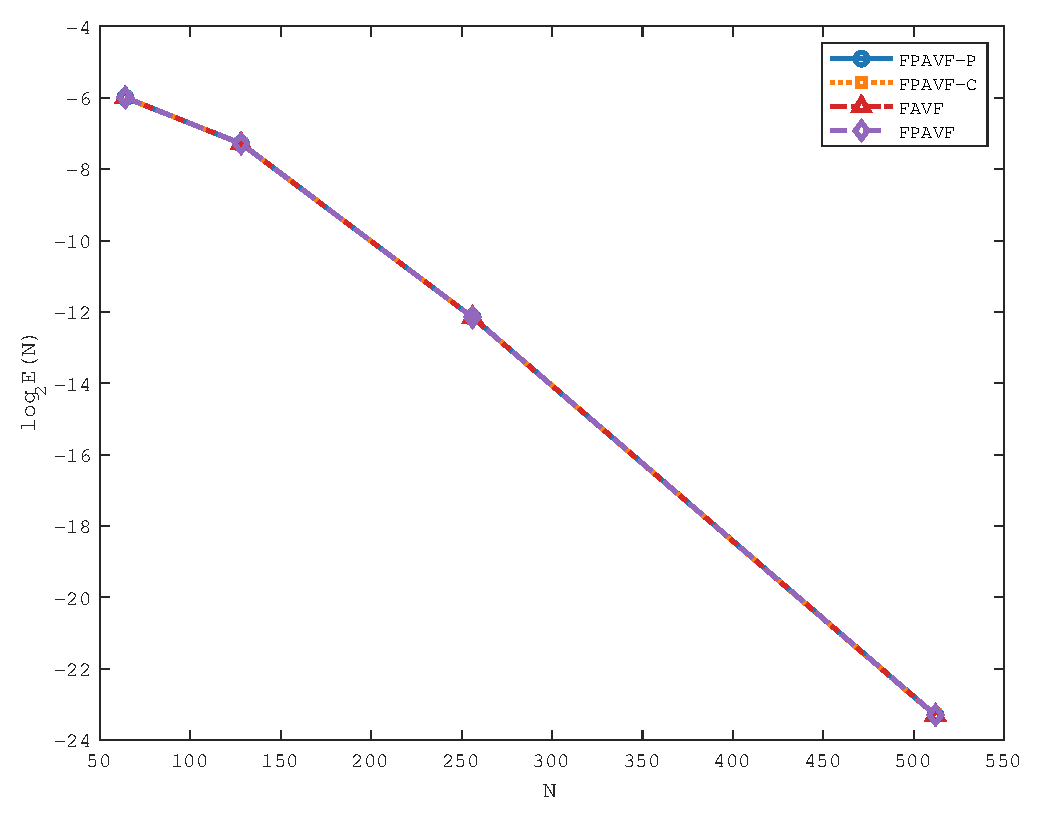
\includegraphics[width=0.35\textwidth]{./figure/exp1_s1.5.eps}
		%\centerline{($b$) Spatial accuracy with $\tau = 10^{-3}.$}
		}\subfigure[$N=128$]{ \centering
		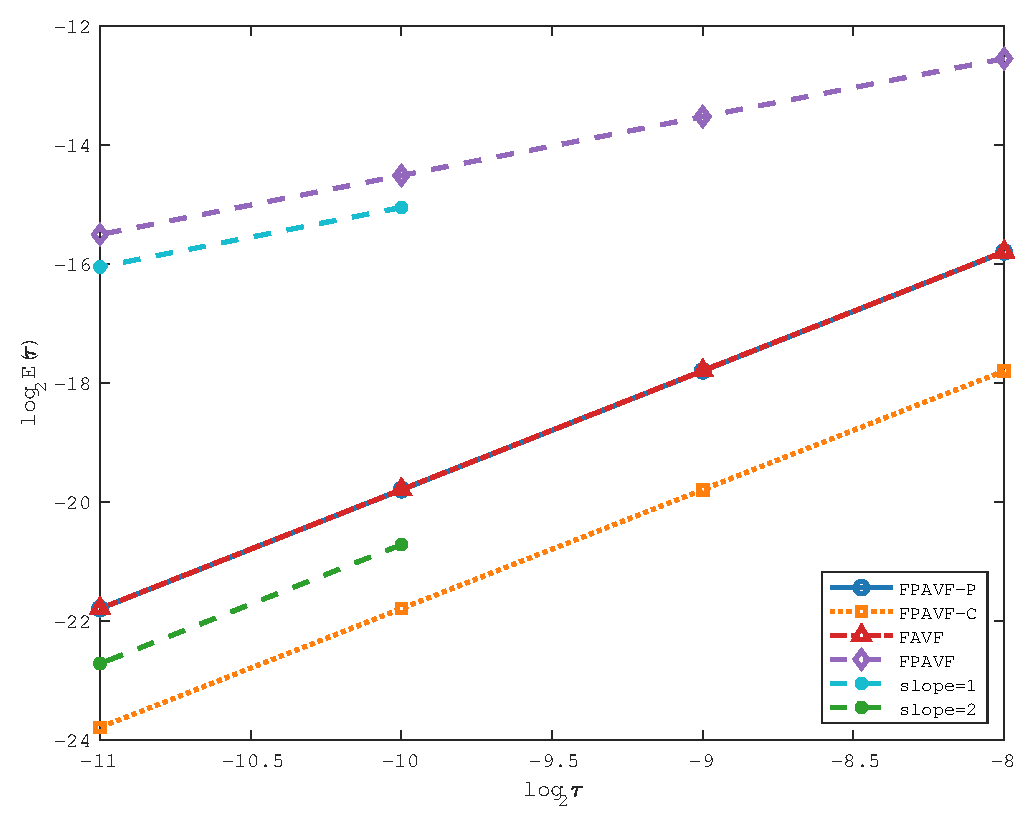
\includegraphics[width=0.35\textwidth]{./figure/exp1_t1.5.eps}
		%\centerline{($a$) Temporal accuracy with $N=128.$}
		}
		% \caption{Convergence orders of four schemes for Example \ref{exp_PAVF:2} with $\alpha=1.5$.}
		\caption{当$\alpha=1.5$时,例 \ref{exp_PAVF:2} 中四种格式的收敛阶.}
		 \label{fig_PAVF:1}
		\end{center}
		\end{figure}
		
		\begin{figure}[H]
		\begin{center}
		\subfigure[$\tau=1/1000$]{ \centering
		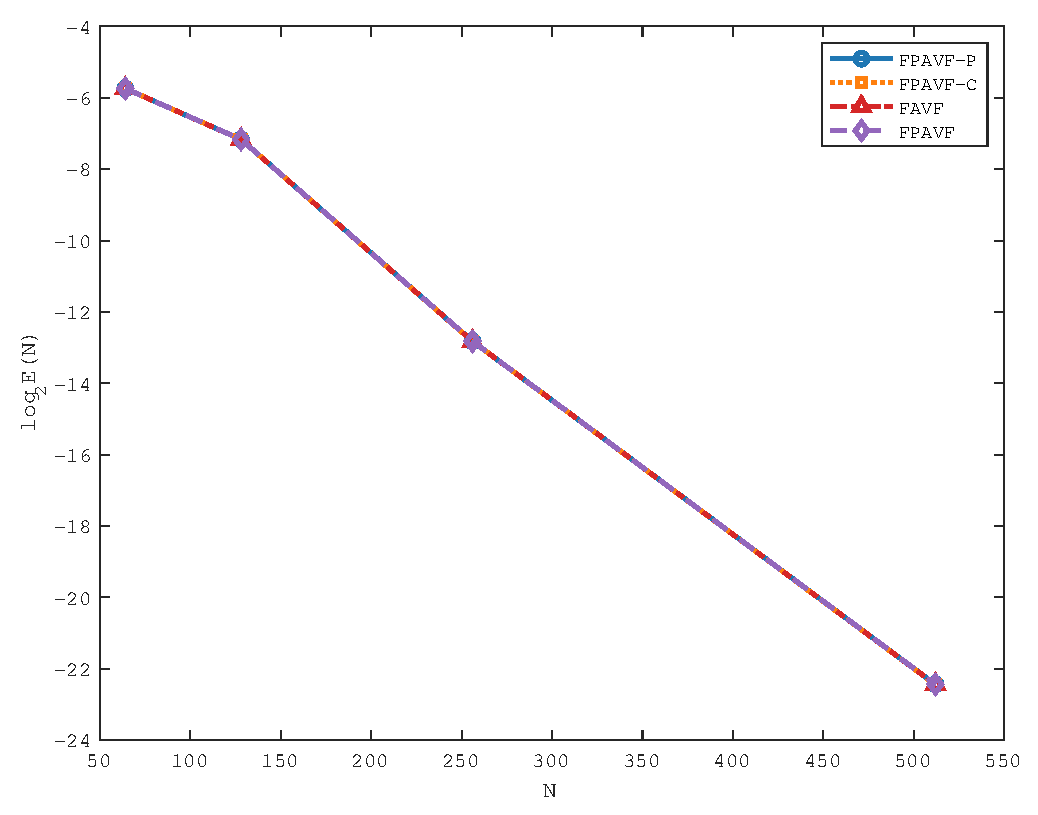
\includegraphics[width=0.35\textwidth]{./figure/exp1_s2.eps}
		%\centerline{($b$) Spatial accuracy with $\tau = 10^{-3}.$}
		}\subfigure[$N=128$]{ \centering
		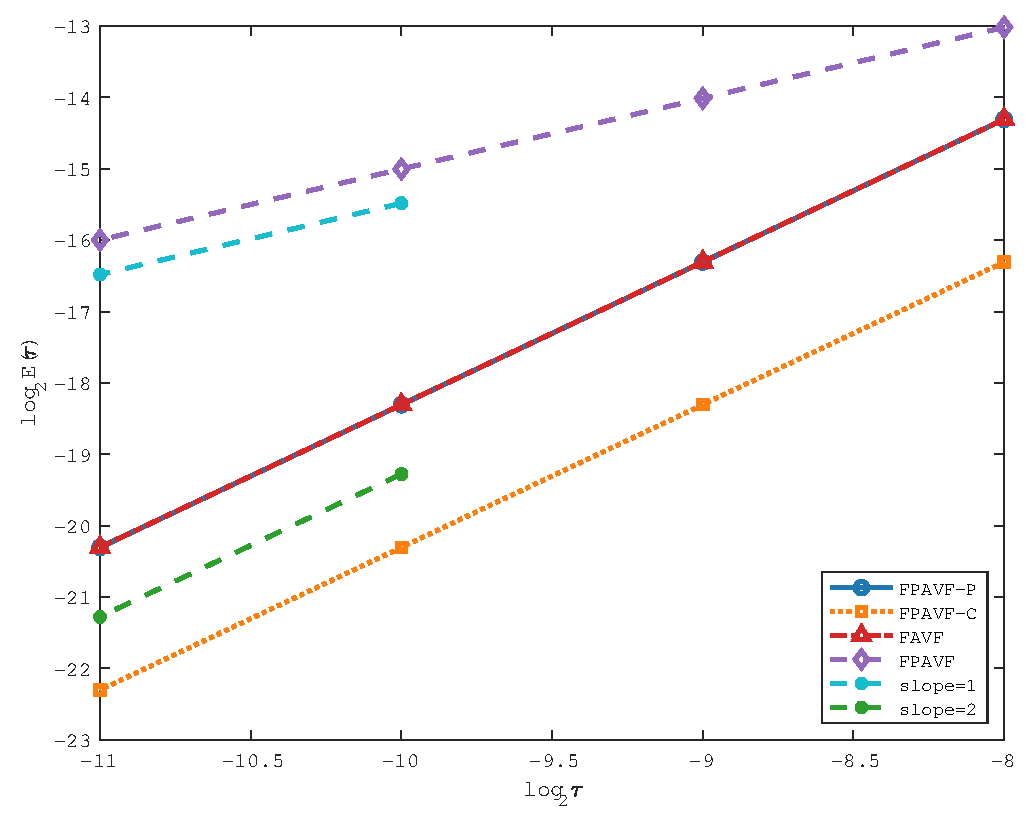
\includegraphics[width=0.35\textwidth]{./figure/exp1_t2.eps}
		%\centerline{($a$) Temporal accuracy with $N=128.$}
		}
		\caption{当$\alpha=2.0$时,例 \ref{exp_PAVF:2} 中四种格式的收敛阶.}
		% \caption{Convergence orders of four schemes for Example \ref{exp_PAVF:2} with $\alpha=2.0$.} \label{fig_PAVF:2}
		\end{center}
		\end{figure}

现在我们关注现有方法的守恒性能.图 \ref{fig_PAVF:3} 显示了在不同 $\alpha$ 值下,通过 $N=512$ 和 $\tau=0.01$ 计算的不同时间段内的离散能量演化情况.可以观察到,特别是在 $\alpha=2$ 的结果中,FPAVF-P、FPAVF、FAVF 和 FPAVF-C 格式计算得到的离散能量均一致收敛到原始能量,而 SAV 方法 \cite{chengConvergenceEnergyconservingScheme2022} 和三层线性隐式差分格式 \cite{ranLinearlyImplicitConservative2016} 的性能较差.这一现象与后者仅保留修改后的能量而不是原始能量是一致的.

\begin{figure}[H]
	\begin{center}
	\subfigure[$\alpha=1.3$]{ \centering
	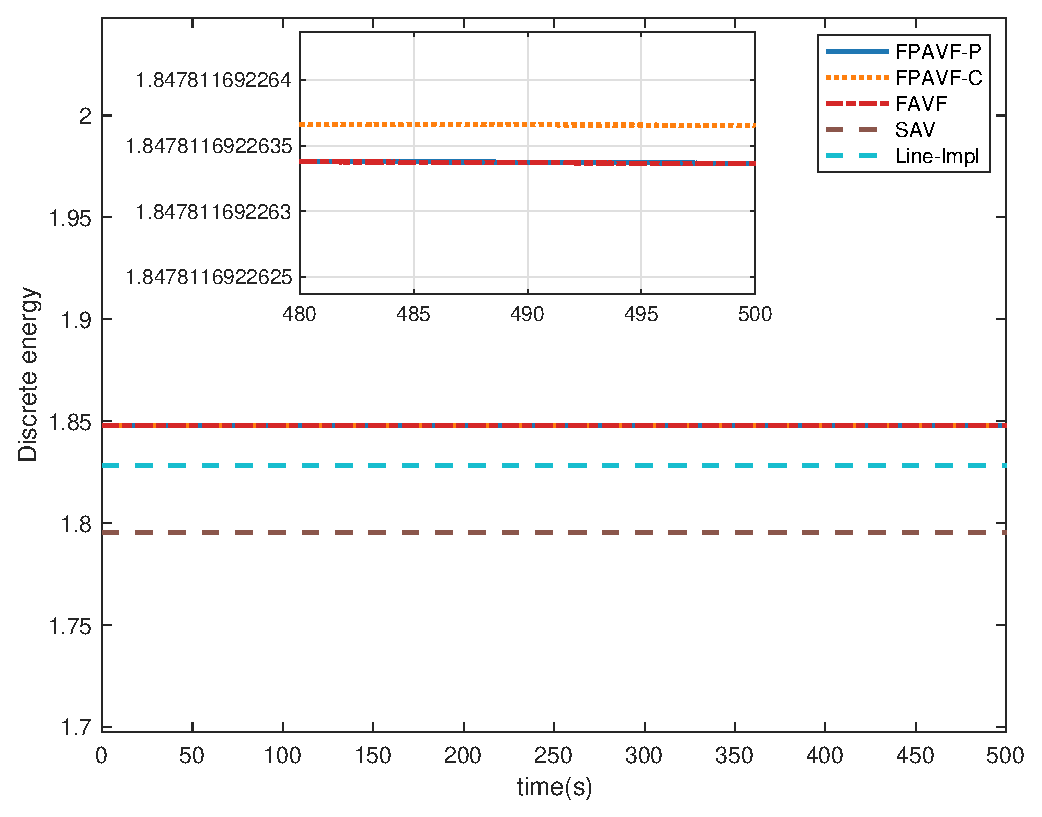
\includegraphics[width=0.4\textwidth]{./figure/exp1_H1.3.eps}
	%\centerline{($a$) $\alpha=1.3$}
	}\subfigure[$\alpha=1.6$]{ \centering
	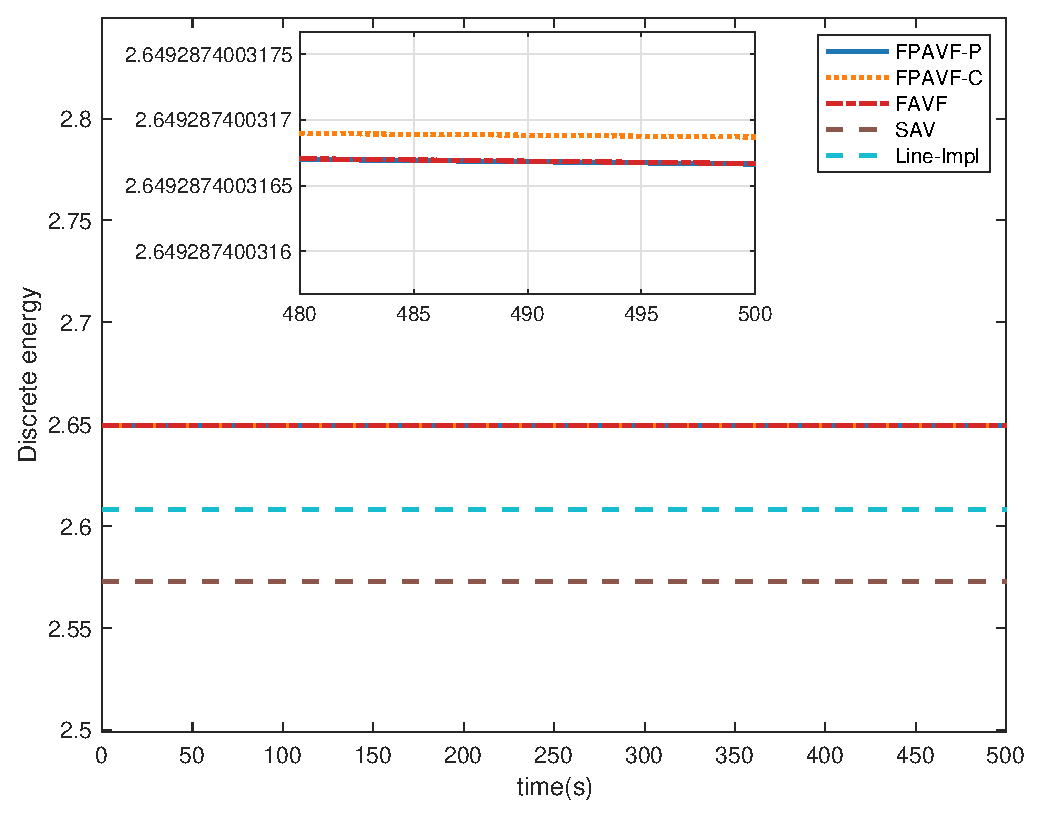
\includegraphics[width=0.4\textwidth]{./figure/exp1_H1.6.eps}
	%\centerline{($b$) $\alpha=1.6$}
	}\\
	\subfigure[$\alpha=1.9$]{ \centering
	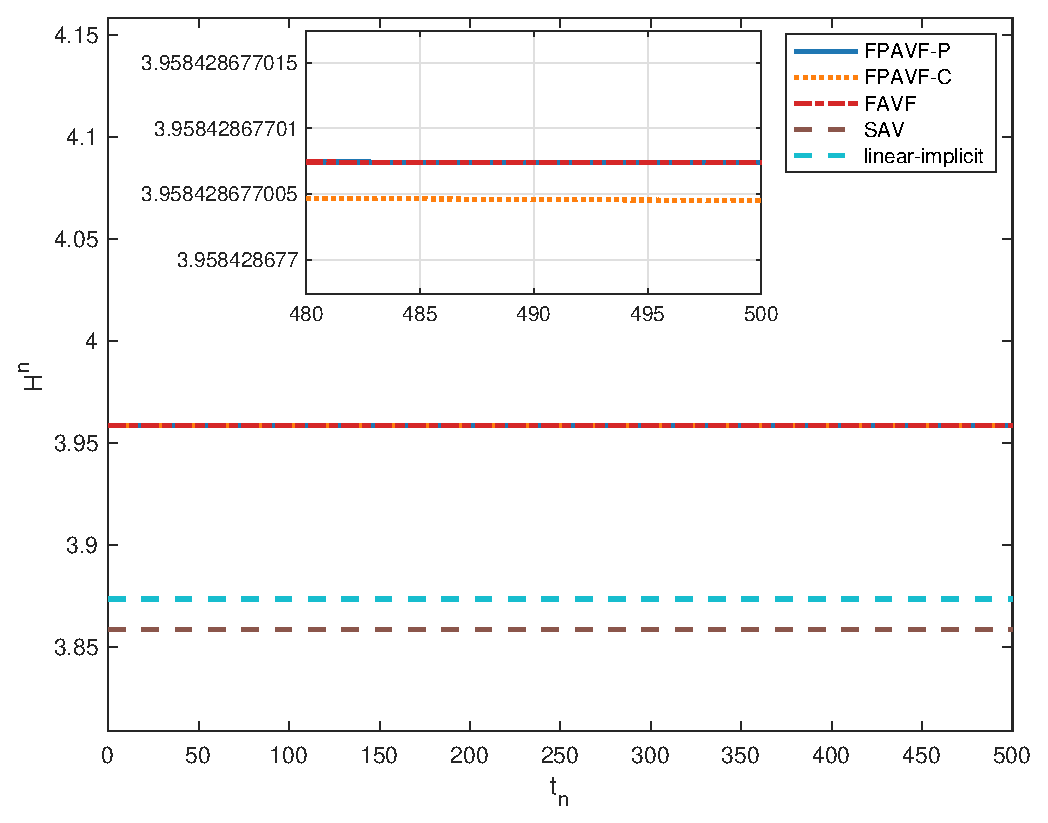
\includegraphics[width=0.4\textwidth]{./figure/exp1_H1.9.eps}
	%\centerline{($d$) $\alpha=2.0$}
	}\subfigure[$\alpha=2.0$]{ \centering
	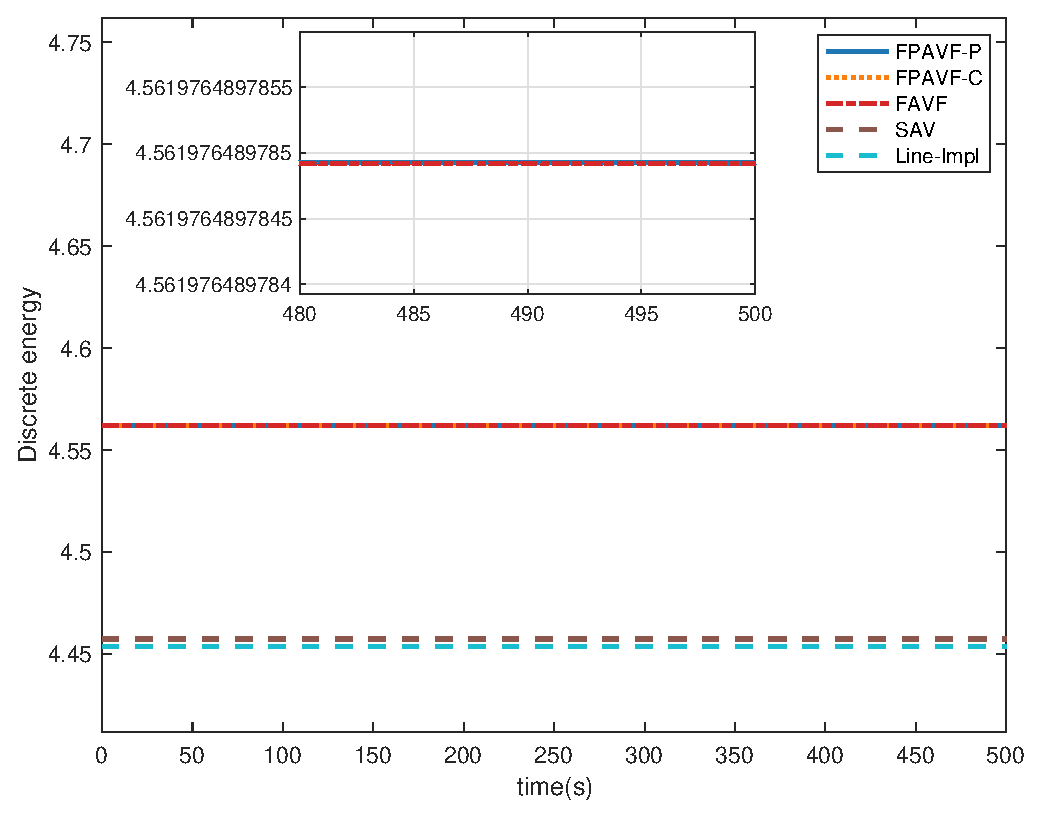
\includegraphics[width=0.4\textwidth]{./figure/exp1_H2.eps}
	%\centerline{($d$) $\alpha=2.0$}
	}
	% \caption{Discrete energy for different $\alpha$ in Example \ref{exp_PAVF:2} with $N = 512$ and $\tau=0.01$.}
	\caption{在例 \ref{exp_PAVF:2} 中,当 $N = 512$ 且 $\tau=0.01$ 时,不同 $\alpha$ 下的离散能量.}
	\label{fig_PAVF:3}
	\end{center}
	\end{figure}

	类似地,图 \ref{fig_PAVF:4} 显示了在不同 $\alpha$ 值下,通过 $N=512$ 和 $\tau=0.01$ 计算的不同时间段内的离散质量演化情况.需要强调的是,SAV 方法不具有质量守恒.
可以看到,FPAVF-P 格式均匀收敛到原始质量,其他方法的性能相对较差,特别是 FAVF 格式,而三层线性隐式差分格式保留了修改后的质量.此外,基于 FPAVF-C 格式的离散质量显示出小幅度的频繁振荡.


\begin{figure}[H]
	\begin{center}
	 \subfigure[$\alpha=1.3$]{ \centering
	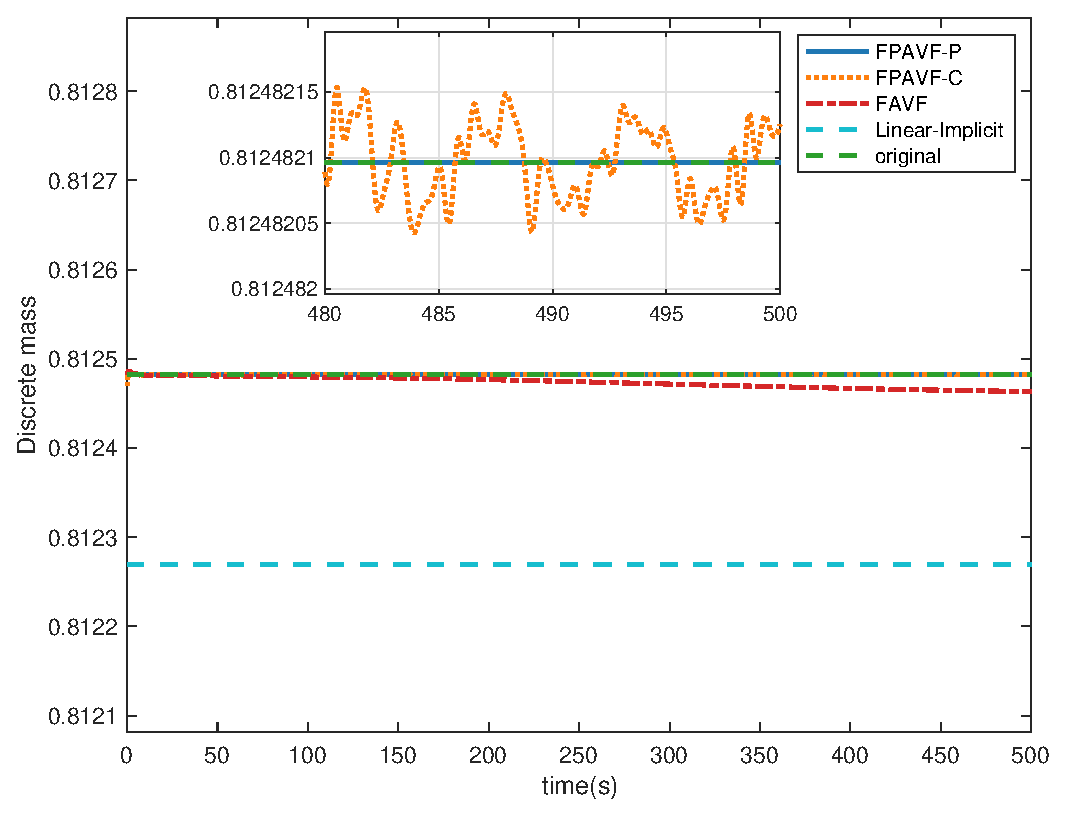
\includegraphics[width=0.4\textwidth]{./figure/exp1_M1.3.eps}
	%\centerline{($a$) $\alpha=1.3$}
	}\subfigure[$\alpha=1.6$]{ \centering
	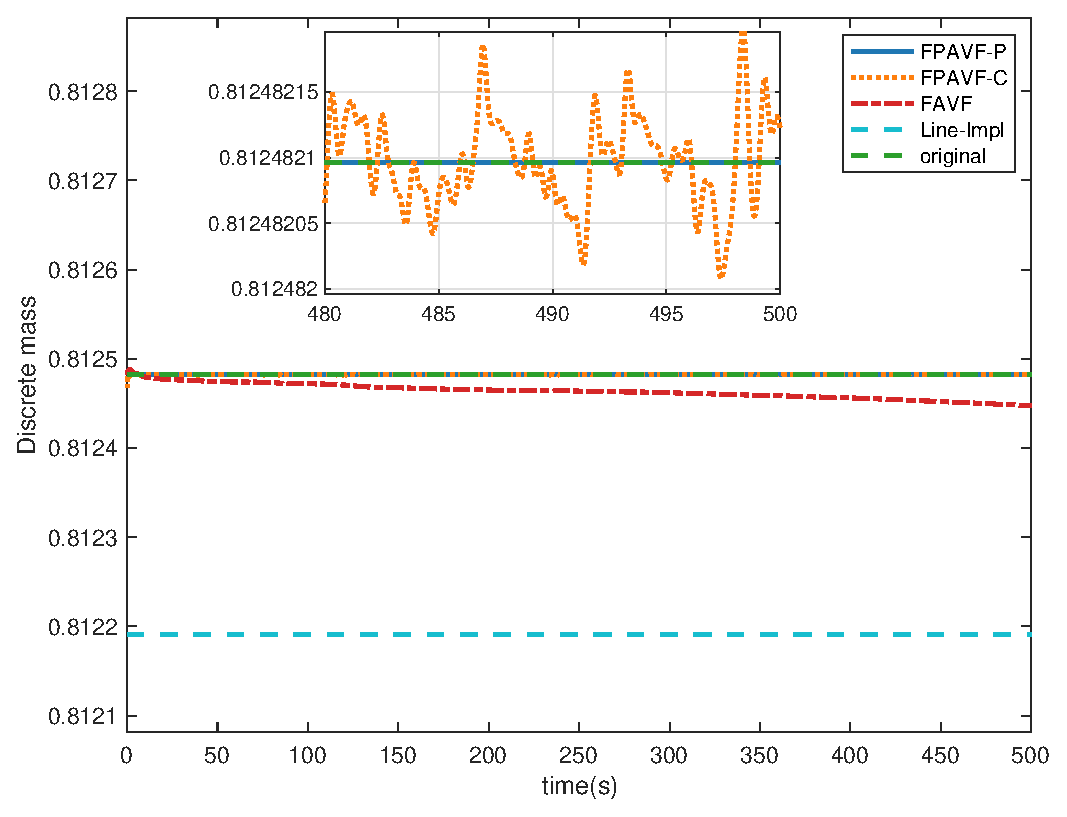
\includegraphics[width=0.4\textwidth]{./figure/exp1_M1.6.eps}
	%\centerline{($b$) $\alpha=1.6$}
	}\\
	 \subfigure[$\alpha=1.9$]{ \centering
	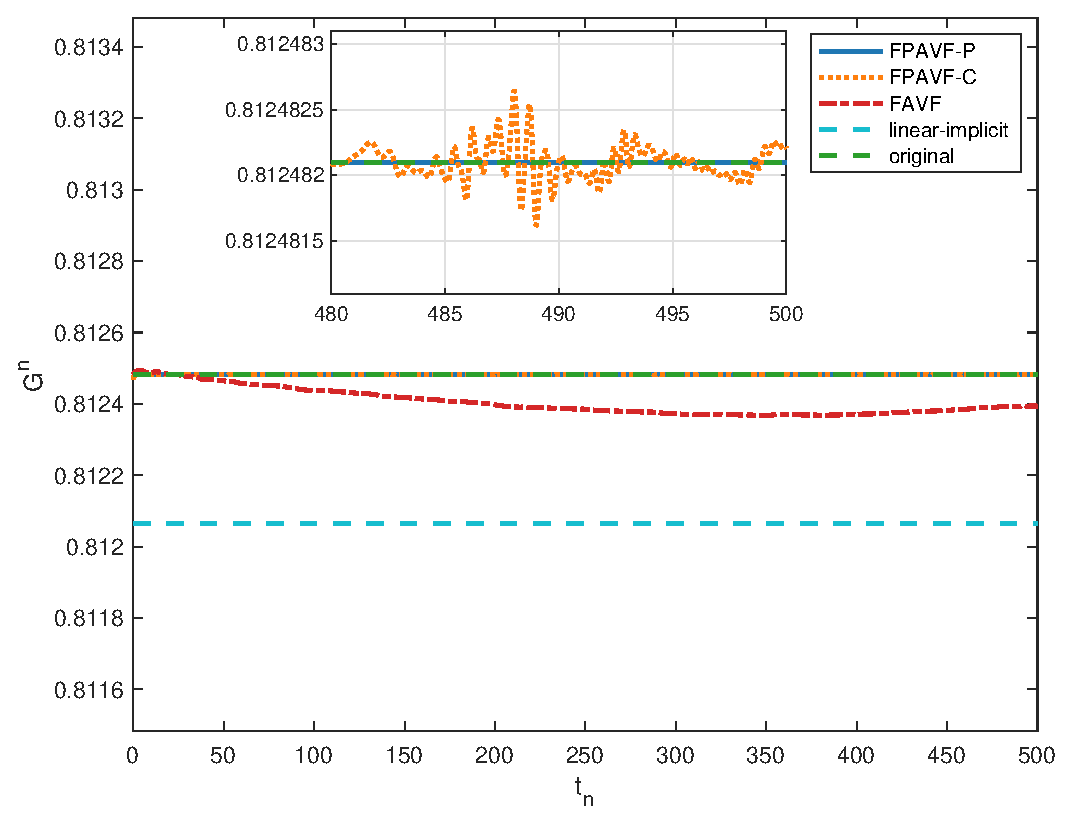
\includegraphics[width=0.4\textwidth]{./figure/exp1_M1.9.eps}
	%\centerline{($c$) $\alpha=1.9$}
	}\subfigure[$\alpha=2.0$]{ \centering
	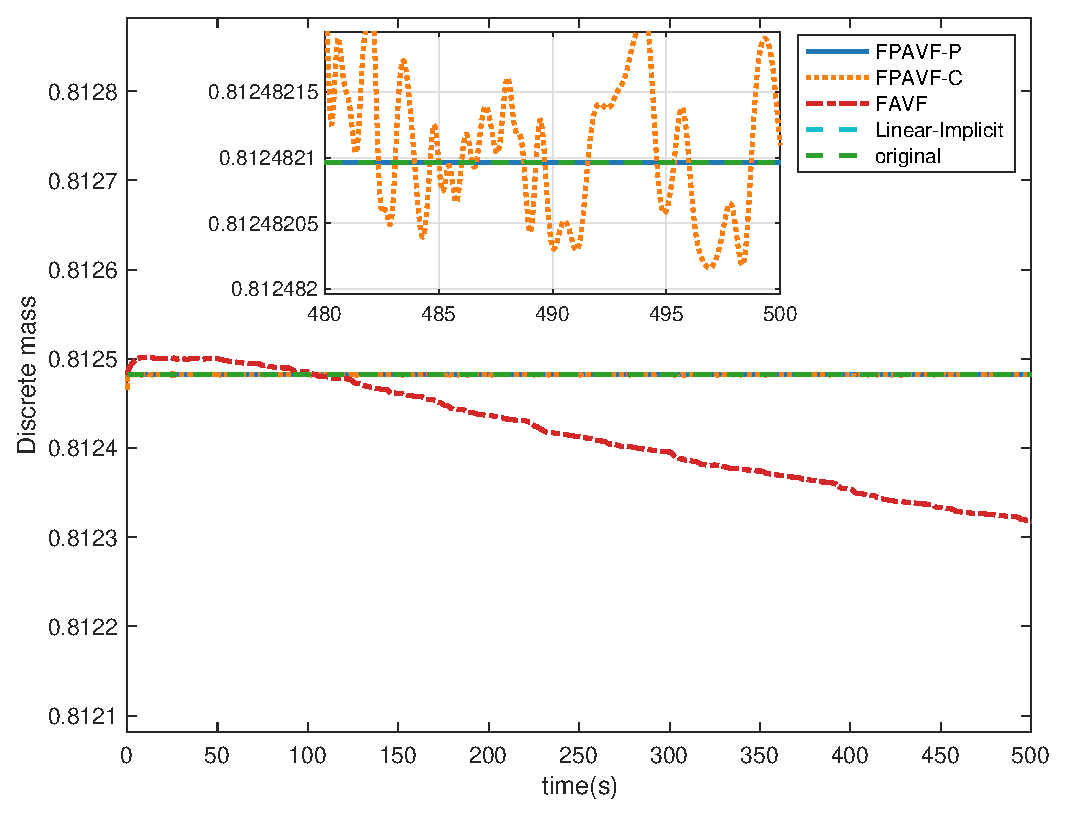
\includegraphics[width=0.4\textwidth]{./figure/exp1_M2.eps}
	%\centerline{($d$) $\alpha=2.0$}
	}
	% \caption{Discrete mass for different $\alpha$ in Example \ref{exp_PAVF:2} with $N = 512$ and $\tau=0.01$.}
	\caption{在例 \ref{exp_PAVF:2} 中,当 $N = 512$ 且 $\tau=0.01$ 时,不同 $\alpha$ 下的离散质量.}
	 \label{fig_PAVF:4}
	\end{center}
	\end{figure}

	更准确地说,表 \ref{tab_PAVF:1} 到表 \ref{tab_PAVF:4} 显示了不同 $\alpha$ 值下不同时间 $t=t_n$ 时的离散能量 $H^n$ 和离散质量 $G^n$ 的值,这些值是通过取 $N=512$ 和 $\tau=0.01$ 获得的.从表 \ref{tab_PAVF:1} 可以看出,提出的四种格式均保留了原始能量,而 SAV 格式和线性隐式差分格式仅保留了修改后的能量.类似地,从表 \ref{tab_PAVF:2} 到表 \ref{tab_PAVF:4},我们观察到 FPAVF-P 格式均匀收敛到原始质量,其他方法性能较差,而三层线性隐式差分格式仅保留了修改后的质量.

	
\begin{table}[H]\small
	\centering
	% \caption{Discrete energy $H^n$ at time $t=t_n$ for Example \ref{exp_PAVF:2} when $\alpha=2$.}
	\caption{在例 \ref{exp_PAVF:2} 中,当 $\alpha=2.0$ 时,时刻 $t=t_n$ 的离散能量 $H^n$.}

	  \begin{tabular}{lllllll}
	  \toprule
       $t$   &FAVF   &FPAVF   &FPAVF-C   &SAV    &Linear-Implicit   &FPAVF-P\\
	  \midrule
	  0     &4.561976489785   &4.561976489785   &4.561976489785   &4.457414815200   &4.453861069486   &4.561976489785 \\
	  10    &4.561976489785   &4.561976489785   &4.561976489785   &4.457414815200   &4.453861069486   &4.561976489785 \\
	  100   &4.561976489785   &4.561976489785   &4.561976489782   &4.457414815197   &4.453861069489   &4.561976489785 \\
	  200   &4.561976489785   &4.561976489785   &4.561976489779   &4.457414815195   &4.453861069492   &4.561976489785 \\
	  300   &4.561976489785   &4.561976489785   &4.561976489776   &4.457414815192   &4.453861069494   &4.561976489785 \\
	  400   &4.561976489785   &4.561976489785   &4.561976489772   &4.457414815190   &4.453861069497   &4.561976489785 \\
	  500   &4.561976489785   &4.561976489785   &4.561976489768   &4.457414815187   &4.453861069500   &4.561976489785 \\
	  \midrule
	  \multicolumn{7}{r}{Original energy:~4.56197648980619} \\
	  \bottomrule
	  \end{tabular}\label{tab_PAVF:1}%
  \end{table}%


\begin{table}[H]\small
	\centering
	% \caption{Discrete mass $G^n$ at time $t=t_n$ for Example \ref{exp_PAVF:2} when $\alpha=1.3$.}
	\caption{在例 \ref{exp_PAVF:2} 中,当 $\alpha=1.3$ 时,时刻 $t=t_n$ 的离散质量 $G^n$.}
	  \begin{tabular}{llllll}
	  \toprule
$t$   &FAVF   &FPAVF   &FPAVF-C   &Linear-Implicit   &FPAVF-P\\
	  \midrule
	  0     &0.812482096011643   &0.812486108372853   &0.812481093228288   &0.812269212105079   &0.812482096009232 \\
	  10    &0.812481652913507   &0.815448411130831   &0.812482228623069   &0.812269212105449   &0.812482096009234 \\
	  100   &0.812479701090339   &0.815337307670638   &0.812482081439882   &0.812269212105119   &0.812482096009236 \\
	  200   &0.812476755660814   &0.815352772611703   &0.812482091028916   &0.812269212105298   &0.812482096009256 \\
	  300   &0.812471706145304   &0.815369448311709   &0.812482102752682   &0.812269212105193   &0.812482096009262 \\
	  400   &0.812466871593141   &0.815375406648485   &0.812482112407629   &0.812269212105361   &0.812482096009263 \\
	  500   &0.812463332390332   &0.815391313914498   &0.812482125179718   &0.812269212105409   &0.812482096009261 \\
	  \midrule
	  \multicolumn{6}{r}{Original mass:~0.812482096009503} \\
	  \bottomrule
	  \end{tabular}\label{tab_PAVF:2}%
  \end{table}%


\begin{table}[H]\small
	\centering
	% \caption{Discrete mass $G^n$ at time $t=t_n$ for Example \ref{exp_PAVF:2} when $\alpha=1.6$.}
	\caption{在例 \ref{exp_PAVF:2} 中,当 $\alpha=1.6$ 时,时刻 $t=t_n$ 的离散质量 $G^n$.}
	\begin{tabular}{llllll}
	  \toprule
$t$   &FAVF   &FPAVF   &FPAVF-C   &Linear-Implicit   &FPAVF-P\\
	  \midrule
	  0     &0.812482096014526   &0.812487932904355   &0.812480637459791   &0.812191342790779   &0.812482096009232 \\
	  10    &0.812479542844467   &0.815290680597744   &0.812482338980161   &0.812191342790869   &0.812482096009234 \\
	  100   &0.812471993678066   &0.814964610988901   &0.812482077830270   &0.812191342790519   &0.812482096009245 \\
	  200   &0.812465076996841   &0.814934135072654   &0.812482168949170   &0.812191342790438   &0.812482096009252 \\
	  300   &0.812461964307183   &0.815026734196011   &0.812482132284732   &0.812191342790211   &0.812482096009255 \\
	  400   &0.812456227758388   &0.815045189971354   &0.812482132454783   &0.812191342790067   &0.812482096009255 \\
	  500   &0.812447472460440   &0.815097180030255   &0.812482122664758   &0.812191342789578   &0.812482096009251 \\
	  \midrule
	  \multicolumn{6}{r}{Original mass:~0.812482096009503} \\
	  \bottomrule
	  \end{tabular}\label{tab_PAVF:3}%
  \end{table}%


\begin{table}[H]\small
	\centering
	% \caption{Discrete mass $G^n$ at time $t=t_n$ for Example \ref{exp_PAVF:2} when $\alpha=2$.}
	\caption{在例 \ref{exp_PAVF:2} 中,当 $\alpha=2.0$ 时,时刻 $t=t_n$ 的离散质量 $G^n$.}
	\begin{tabular}{llllll}
	  \toprule
$t$   &FAVF   &FPAVF   &FPAVF-C   &Linear-Implicit   &FPAVF-P\\
	  \midrule
	  0     &0.812482096027426   &0.812492566135382   &0.812479480708946   &0.812007279829162   &0.812482096009232 \\
	  10    &0.812501574603936   &0.815690689466538   &0.812482208549750   &0.812007279829185   &0.812482096009233 \\
	  100   &0.812485179319911   &0.815559529804266   &0.812482224295188   &0.812007279829068   &0.812482096009234 \\
	  200   &0.812436598720768   &0.815737264057778   &0.812482177481325   &0.812007279828906   &0.812482096009234 \\
	  300   &0.812395565737519   &0.815914179675223   &0.812482122649446   &0.812007279828999   &0.812482096009235 \\
	  400   &0.812353830841431   &0.816227202656059   &0.812482101787071   &0.812007279828969   &0.812482096009235 \\
	  500   &0.812317849493374   &0.816336221770707   &0.812482109657662   &0.812007279829037   &0.812482096009234 \\
	  \midrule
	  \multicolumn{6}{r}{Original mass:~0.812482096009503} \\
	  \bottomrule
	  \end{tabular}\label{tab_PAVF:4}%
  \end{table}%

  由于对于 $\alpha\neq 2$,原始能量的计算不太容易,我们从相对误差的角度验证了离散守恒定律,见图 \ref{fig_PAVF:5} 到图 \ref{fig_PAVF:6}.同样,这些图表显示 FPAVF-P 格式在保持原始质量方面具有最佳性能.随着 $\alpha$ 的增加,它在保持原始能量方面的性能将更好.这些观察结果与我们之前的理论结果一致.

  \begin{figure}[H]
	\begin{center}
	 \subfigure[$\alpha=1.3$]{ \centering
	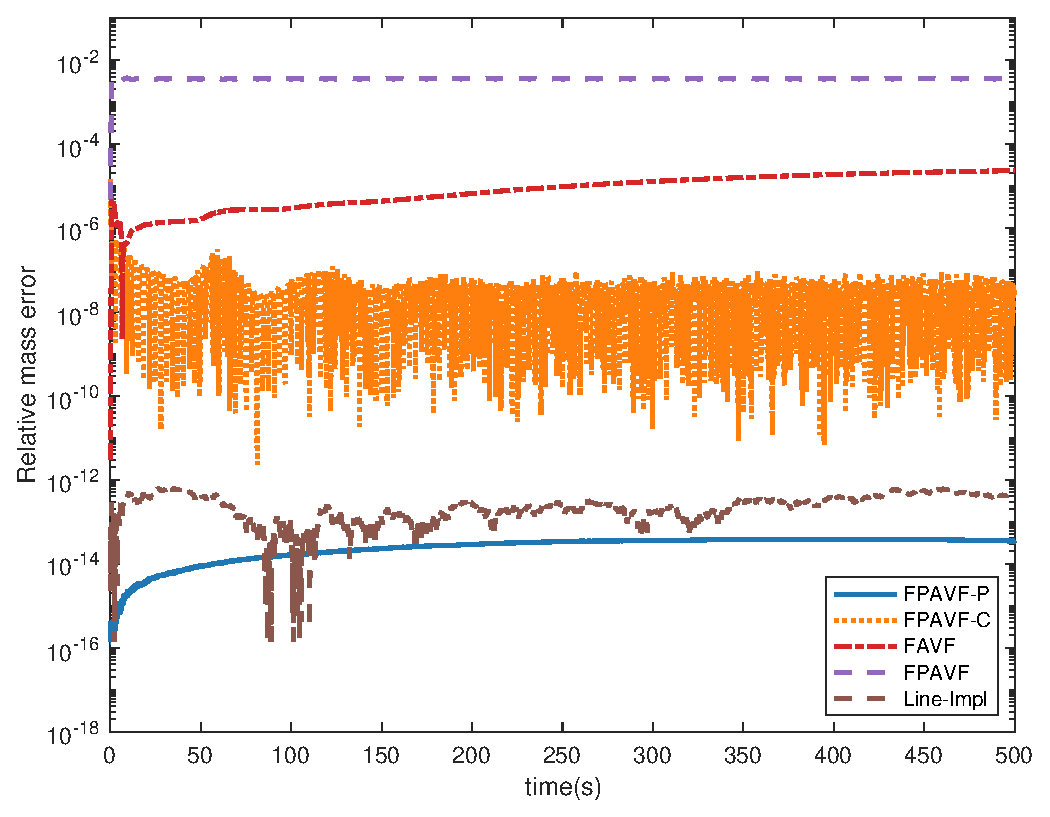
\includegraphics[width=0.3\textwidth]{./figure/exp1_RM1.3.eps}
	%\centerline{($a$) $\alpha=1.3$}
	}\subfigure[$\alpha=1.6$]{ \centering
	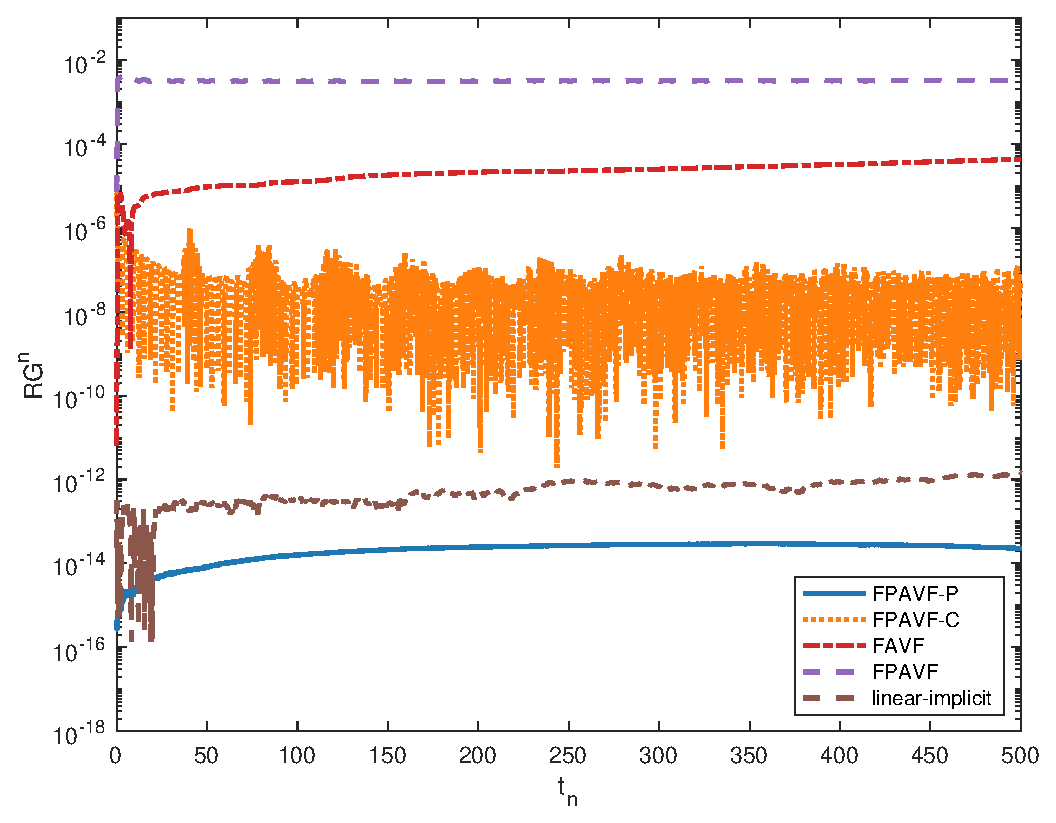
\includegraphics[width=0.3\textwidth]{./figure/exp1_RM1.6.eps}
	%\centerline{($b$) $\alpha=1.6$}
	}\subfigure[$\alpha=1.9$]{ \centering
	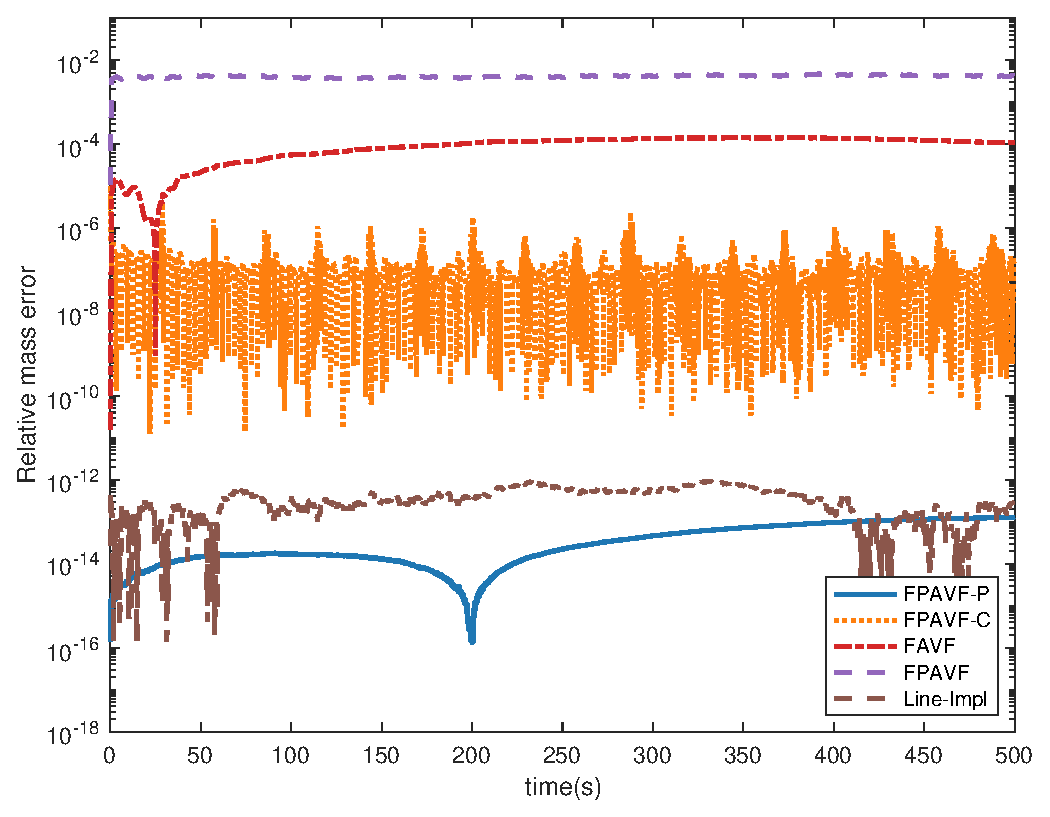
\includegraphics[width=0.3\textwidth]{./figure/exp1_RM1.9.eps}
	%\centerline{($c$) $\alpha=1.9$}
	}
	% \caption{The relative errors of discrete mass for different $\alpha$ in Example \ref{exp_PAVF:2} with $N = 512$ and $\tau=0.01$.}
	\caption{在例 \ref{exp_PAVF:2} 中,当 $N = 512$ 且 $\tau=0.01$ 时,不同 $\alpha$ 下的离散质量相对误差}
	\label{fig_PAVF:5}
	\end{center}
	\end{figure}
	
	\begin{figure}[H]
	\begin{center}
	 \subfigure[$\alpha=1.3$]{ \centering
	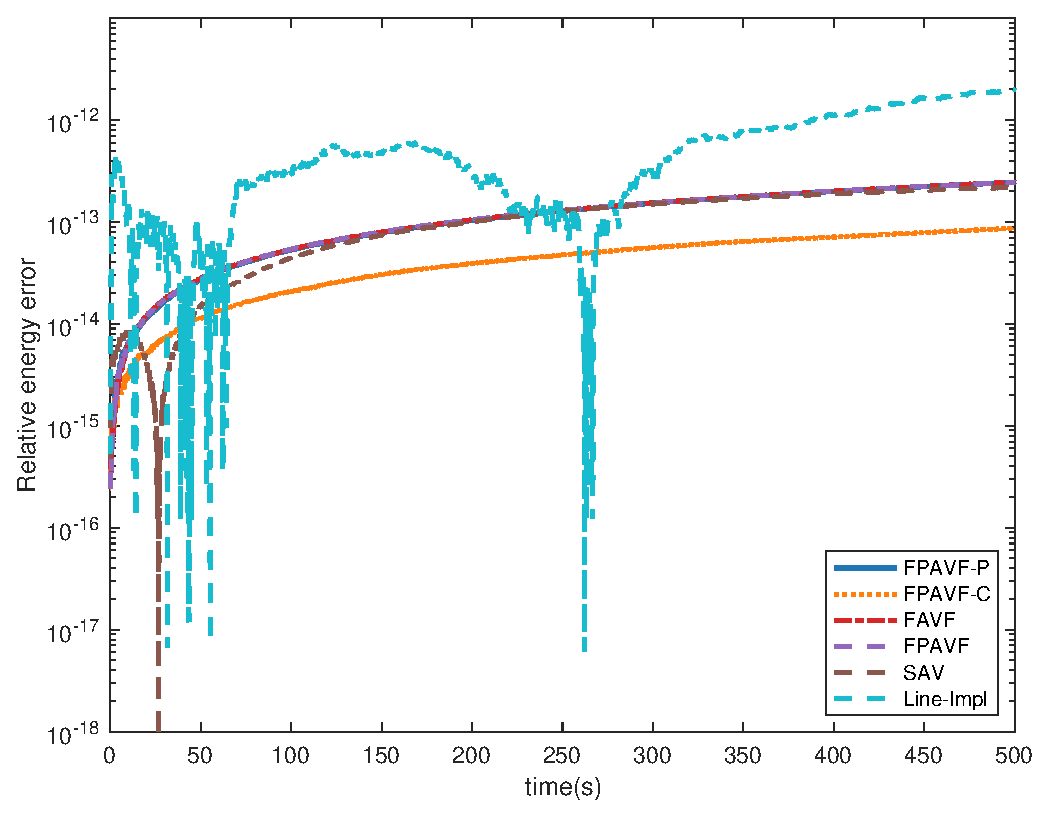
\includegraphics[width=0.3\textwidth]{./figure/exp1_RH1.3.eps}
	%\centerline{($a$) $\alpha=1.3$}
	}\subfigure[$\alpha=1.6$]{ \centering
	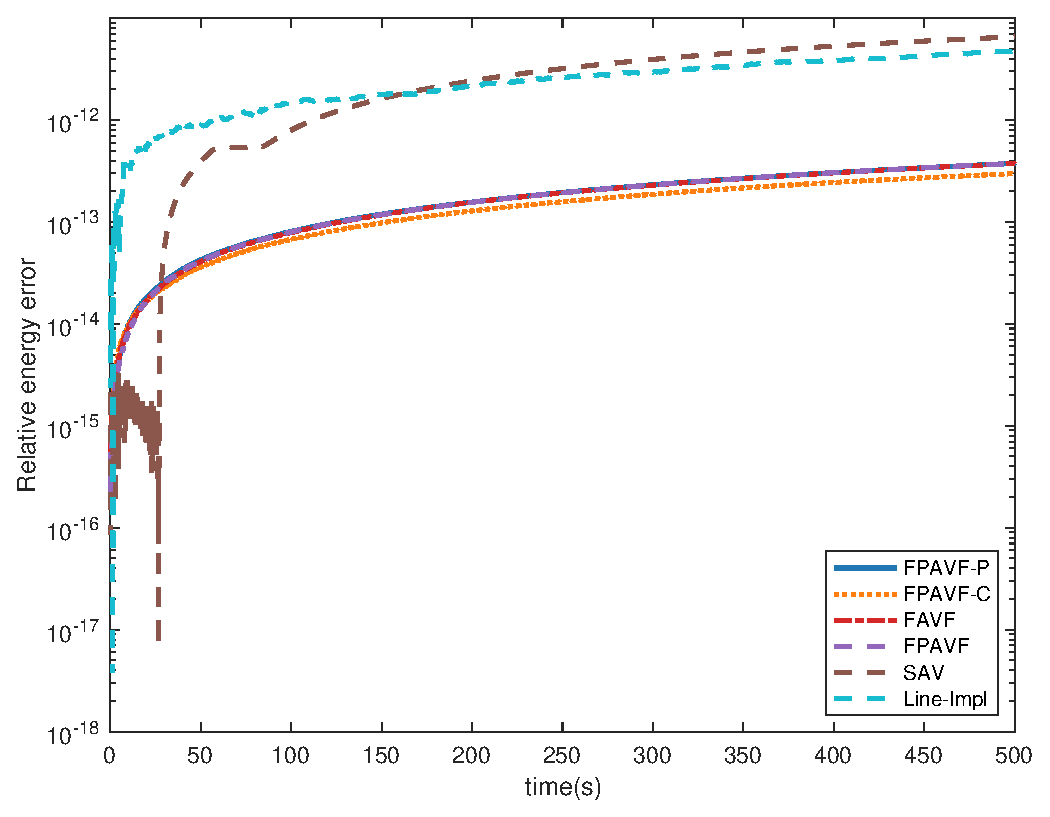
\includegraphics[width=0.3\textwidth]{./figure/exp1_RH1.6.eps}
	%\centerline{($b$) $\alpha=1.6$}
	} \subfigure[$\alpha=1.9$]{ \centering
	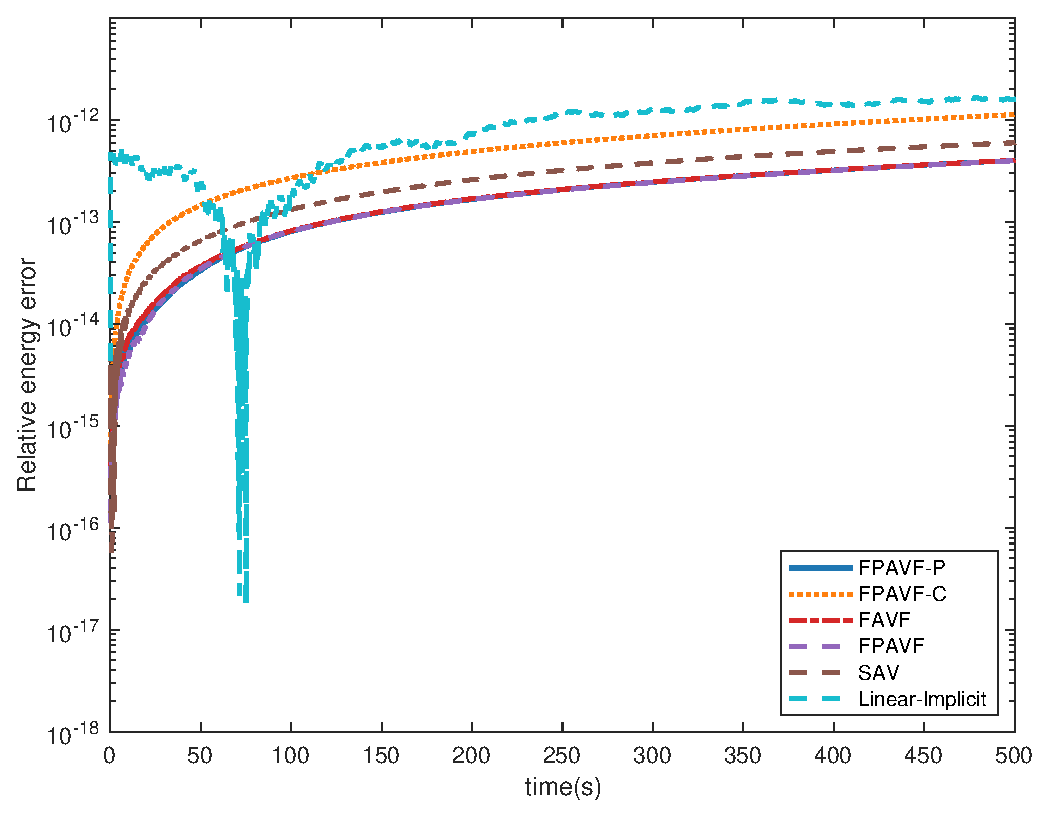
\includegraphics[width=0.3\textwidth]{./figure/exp1_RH1.9.eps}
	%\centerline{($c$) $\alpha=1.9$}
	}
	% \caption{The relative errors of discrete energy for different $\alpha$ in Example \ref{exp_PAVF:2} with $N = 512$ and $\tau=0.01$.} 
	\caption{在例 \ref{exp_PAVF:2} 中,当 $N = 512$ 且 $\tau=0.01$ 时,不同 $\alpha$ 下的离散能量相对误差}\label{fig_PAVF:6}
	\end{center}
	\end{figure}
	\begin{example}\label{exp_PAVF:4}
		现在我们考虑带有初始值的二维非线性分数薛定谔波动方程 \eqref{eq_1}-\eqref{eq_3}:
		\begin{equation}\label{eq_PAVF_110}
		u(x,y, 0)=\mbox{sech}\left(x^2+y^2\right), u_t(x,y, 0)=\sin (x+y) \mbox{sech}\left(-2(x^2+y^2)\right), (x,y,t)\in  \Omega\times[0, T],
		\end{equation}
		其中 $\Omega=[-5,5] \times[-5,5]$.
		\end{example}
	类似于一维情况,我们首先计算 FPAVF-P、FPAVF、FAVF 和 FPAVF-C 格式在 $\alpha=1.5$ 和 $\alpha=2.0$ 时 $T=1$ 的收敛阶.误差变化如图 \ref{fig_PAVF:7} 到图 \ref{fig_PAVF:8} 所示.我们可以清晰地观察到这四种格式在空间上都具有谱精度,而 FPAVF 格式在时间上表现出一阶精度,其他格式在时间上表现出二阶精度.

	
\begin{figure}[H]
	\begin{center}
	\subfigure[$\tau=1/1000$]{ \centering
	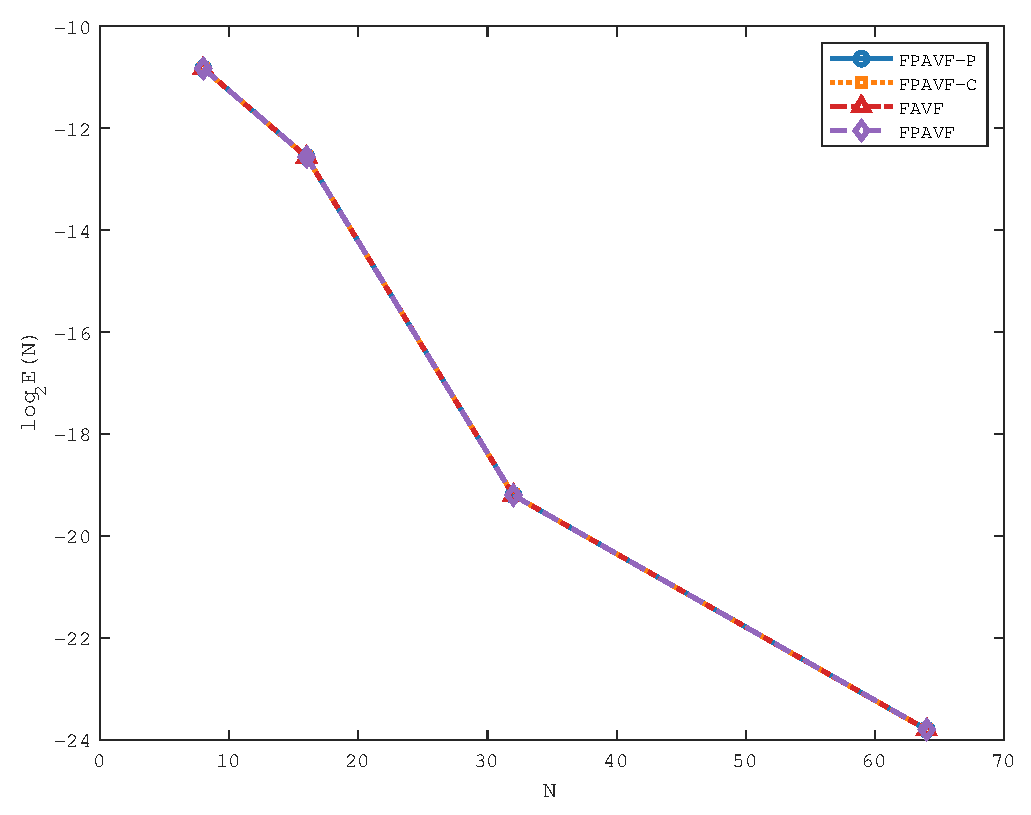
\includegraphics[width=0.35\textwidth]{./figure/exp2_s1.5.eps}
	%\centerline{($b$) Spatial accuracy with $\tau = 10^{-3}.$}
	}\subfigure[$N=16$]{ \centering
	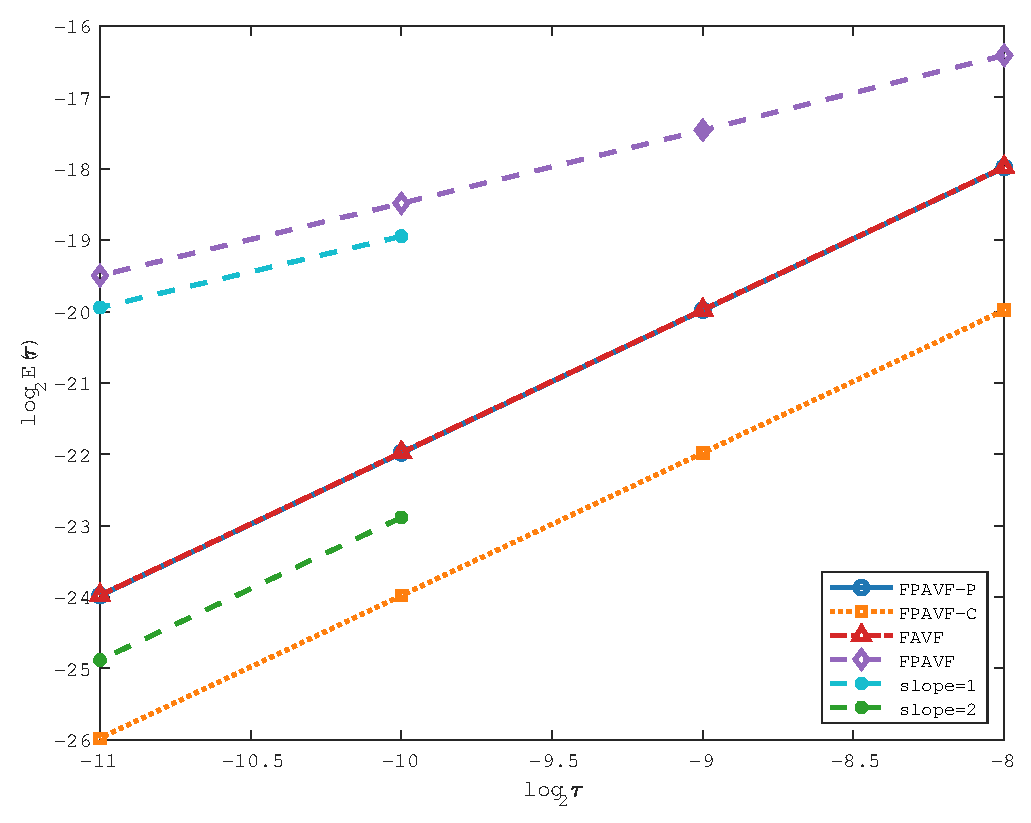
\includegraphics[width=0.35\textwidth]{./figure/exp2_t1.5.eps}
	%\centerline{($a$) Temporal accuracy with $N=128.$}
	}
	% \caption{Convergence orders of four schemes for Example \ref{exp_PAVF:4} with $\alpha=1.5$.} 
	\caption{当$\alpha=1.5$时,例 \ref{exp_PAVF:4} 中四种格式的收敛阶.}
	\label{fig_PAVF:7}
	\end{center}
	\end{figure}
	
	\begin{figure}[H]
	\begin{center}
	\subfigure[$\tau=1/1000$]{ \centering
	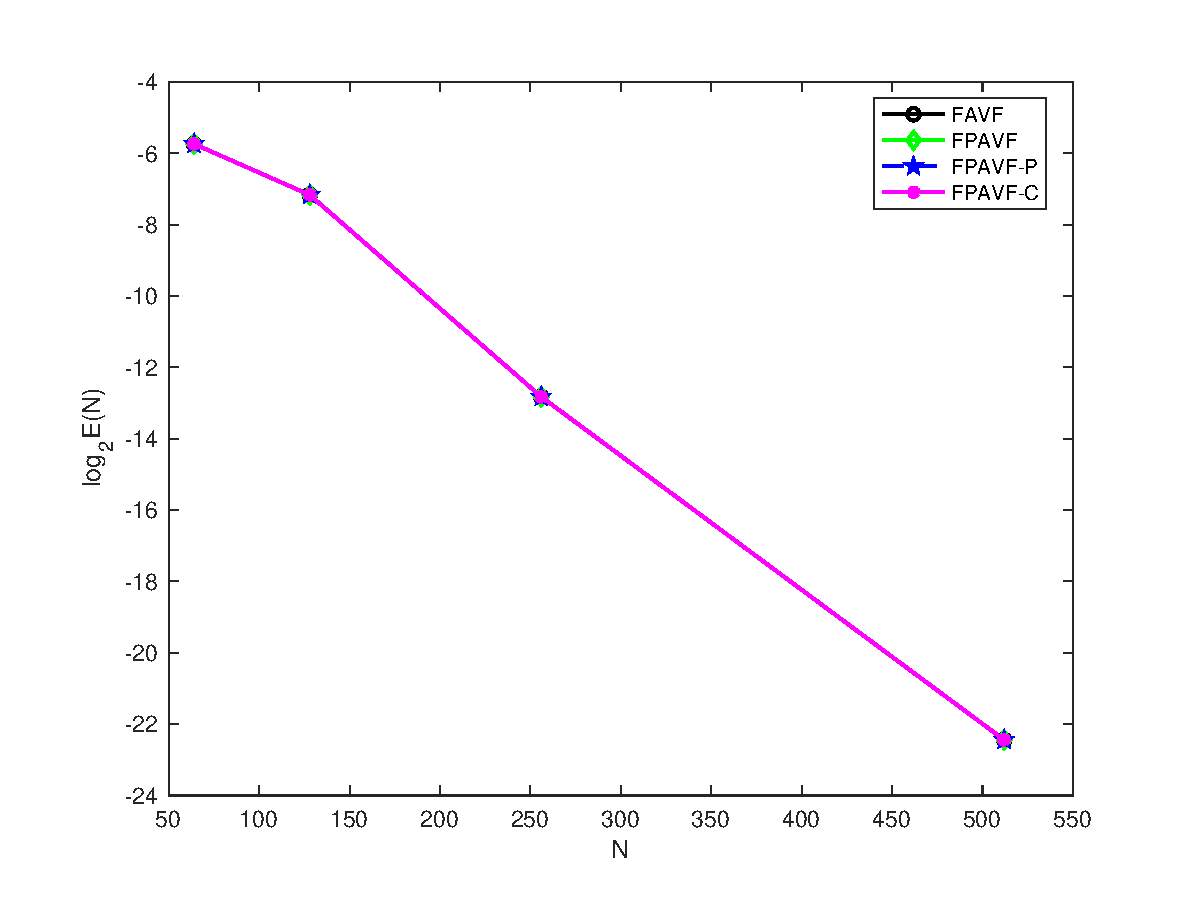
\includegraphics[width=0.35\textwidth]{./figure/exp2_s2.eps}
	%\centerline{($b$) Spatial accuracy with $\tau = 10^{-3}.$}
	}\subfigure[$N=16$]{ \centering
	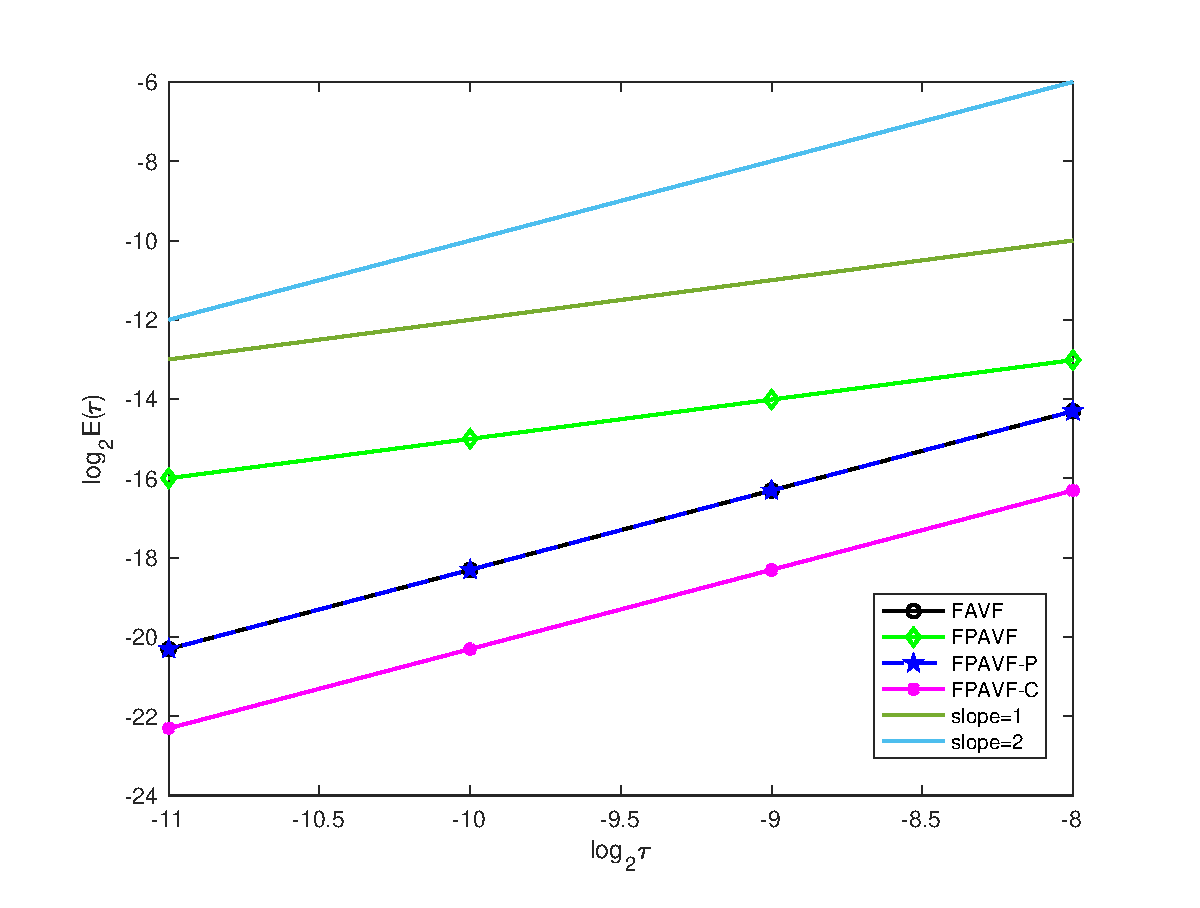
\includegraphics[width=0.35\textwidth]{./figure/exp2_t2.eps}
	%\centerline{($a$) Temporal accuracy with $N=128.$}
	}
	% \caption{Convergence orders of four schemes for Example \ref{exp_PAVF:4} with $\alpha=2.0$.}
	\caption{当$\alpha=2.0$时,例 \ref{exp_PAVF:4} 中四种格式的收敛阶.}
	 \label{fig_PAVF:8}
	\end{center}
	\end{figure}

	为了比较与现有方法的结构保持能力,我们首先计算了原始质量和能量.注意到原始质量 $G(t)$ 与 $\alpha$ 无关,通过使用高斯数值积分,我们得到了任何 $\alpha$ 下的原始质量 $G(0)=3.14159265323701$.类似地,我们可以得到 $\alpha=2$ 时的原始能量 $E(0)=3.22697078976648$.

与一维问题不同,二维情况下没有三级线性隐式格式,因此我们只比较了本文提出的 SAV 方法、FPAVF-P、FAVF 和 FPAVF-C 格式的性能.图 \ref{fig_PAVF:9} 到图 \ref{fig_PAVF:10} 展示了在不同 $\alpha$ 下通过 $N=64$ 和 $\tau=0.01$ 计算的离散质量和离散能量的演变.图 \ref{fig_PAVF:11} 到图 \ref{fig_PAVF:12} 展示了随时间变化的离散质量和能量的相对误差的变化.我们可以观察到,FPAVF-P 格式在原始质量上收敛得很好,其他三种方法性能较差,尤其是 FAVF 格式和 FPAVF 格式(FPAVF 格式的结果这里没有显示因为它更糟糕).而本文提出的三种格式都能很好地保持原始能量不变,而 SAV 方法只能保持一个修正的能量.这些现象再次确认了我们理论结果的正确性.


\begin{figure}[H]
	\begin{center}
	 \subfigure[$\alpha=1.3$]{ \centering
	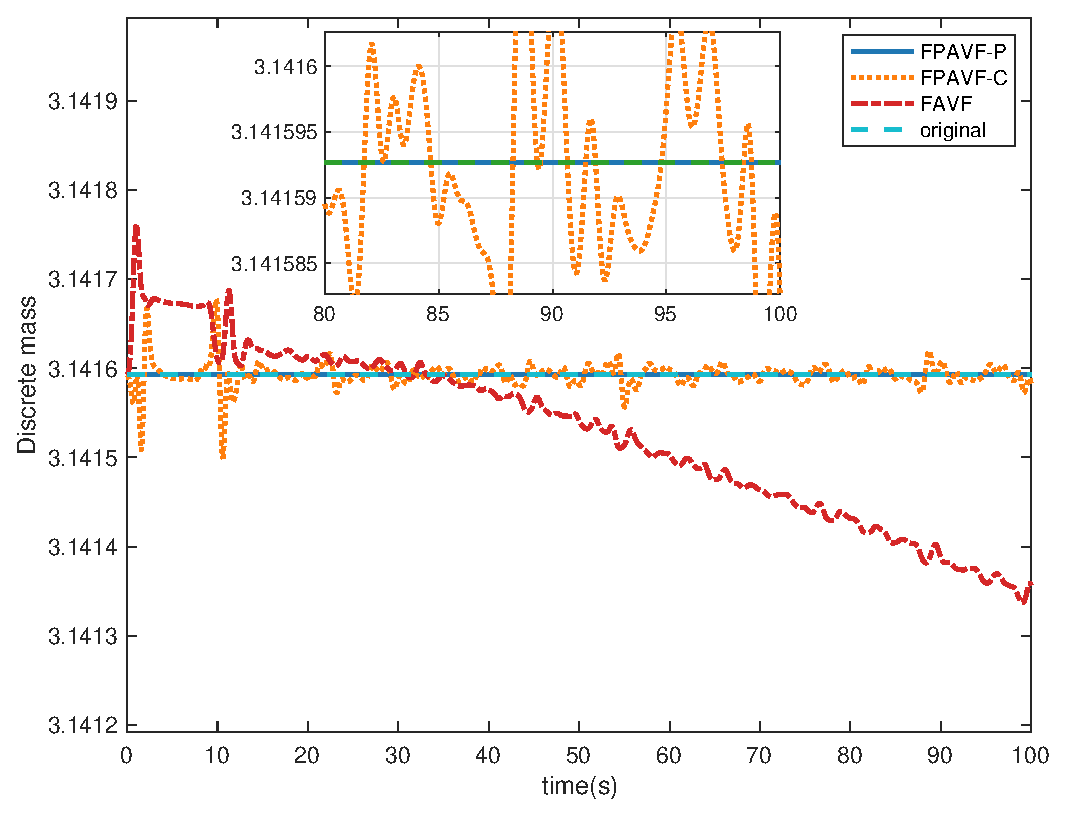
\includegraphics[width=0.3\textwidth]{./figure/exp2_M1.3.eps}
	%\centerline{($a$) $\alpha=1.3$}
	}\subfigure[$\alpha=1.6$]{ \centering
	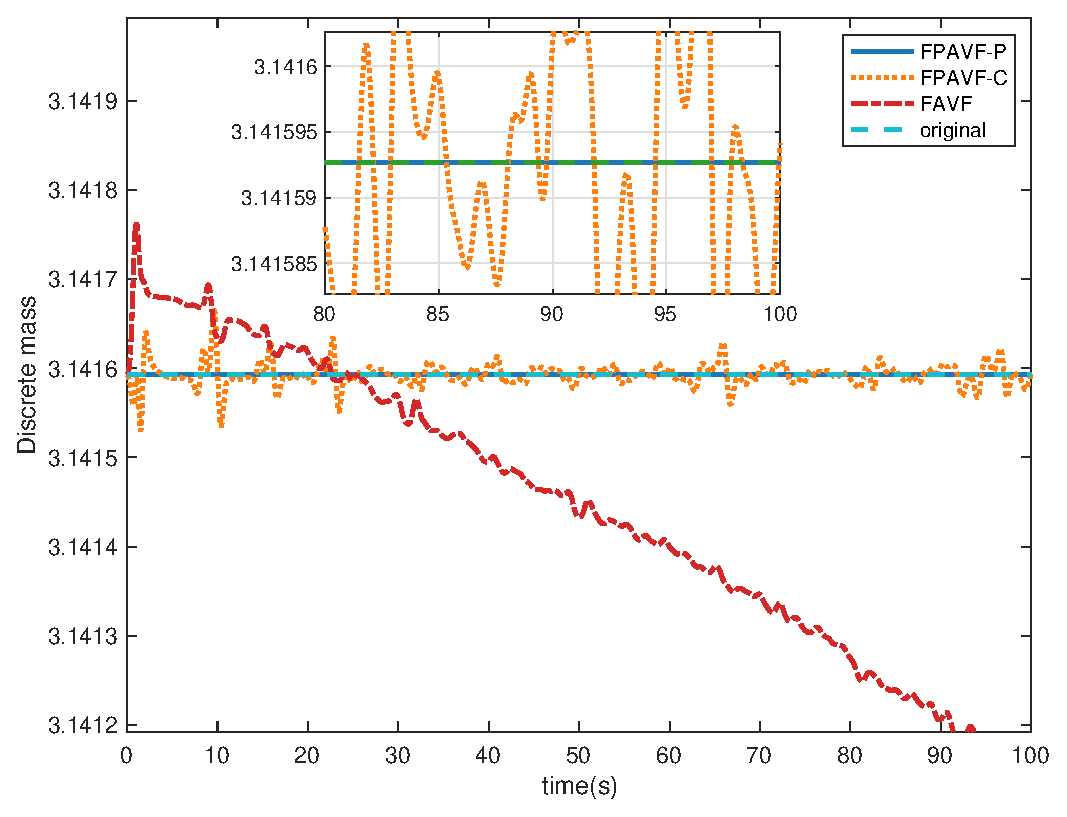
\includegraphics[width=0.3\textwidth]{./figure/exp2_M1.6.eps}
	%\centerline{($b$) $\alpha=1.6$}
	}\\
	 \subfigure[$\alpha=1.9$]{ \centering
	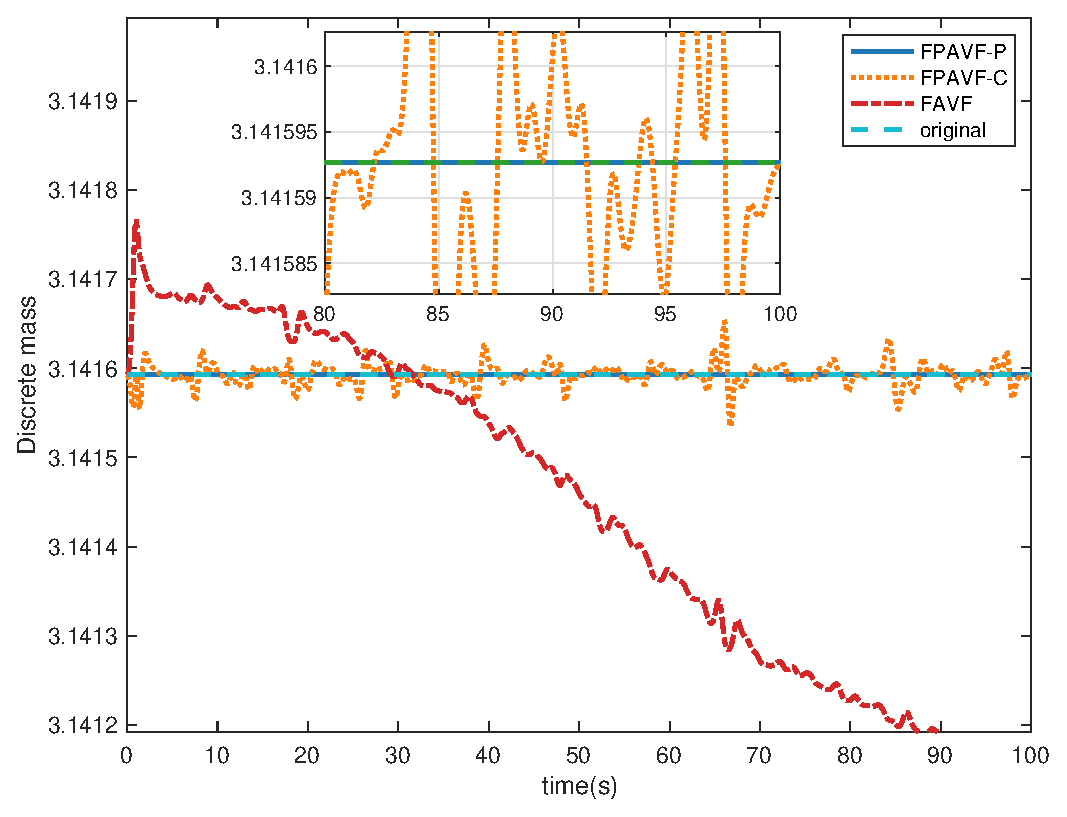
\includegraphics[width=0.3\textwidth]{./figure/exp2_M1.9.eps}
	%\centerline{($c$) $\alpha=1.9$}
	}\subfigure[$\alpha=2.0$]{ \centering
	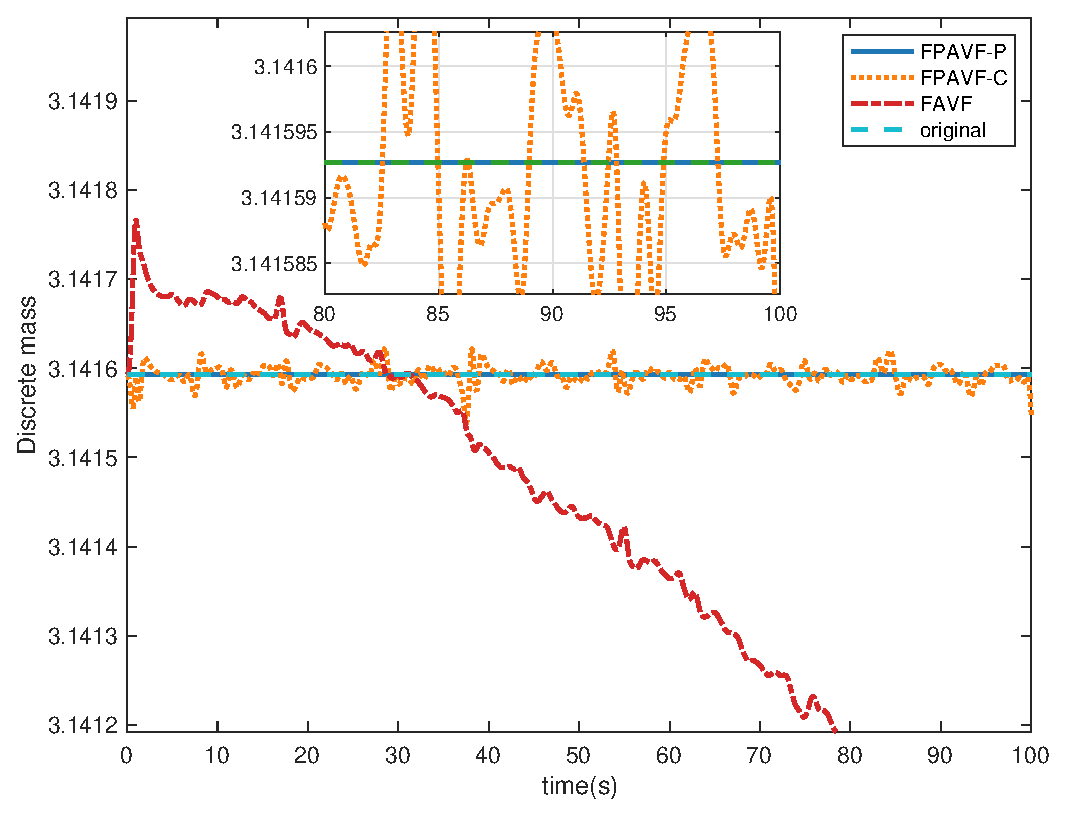
\includegraphics[width=0.3\textwidth]{./figure/exp2_M2.eps}
	%\centerline{($d$) $\alpha=2.0$}
	}
	% \caption{Discrete mass for different $\alpha$ in Example \ref{exp_PAVF:4} with $N = 64$ and $\tau=0.01$.} 
	\caption{在例 \ref{exp_PAVF:4} 中,当 $N = 64$ 且 $\tau=0.01$ 时,不同 $\alpha$ 下的离散质量.}
	\label{fig_PAVF:9}
	\end{center}
	\end{figure}

\begin{figure}[H]
	\begin{center}
	\subfigure[$\alpha=1.3$]{ \centering
	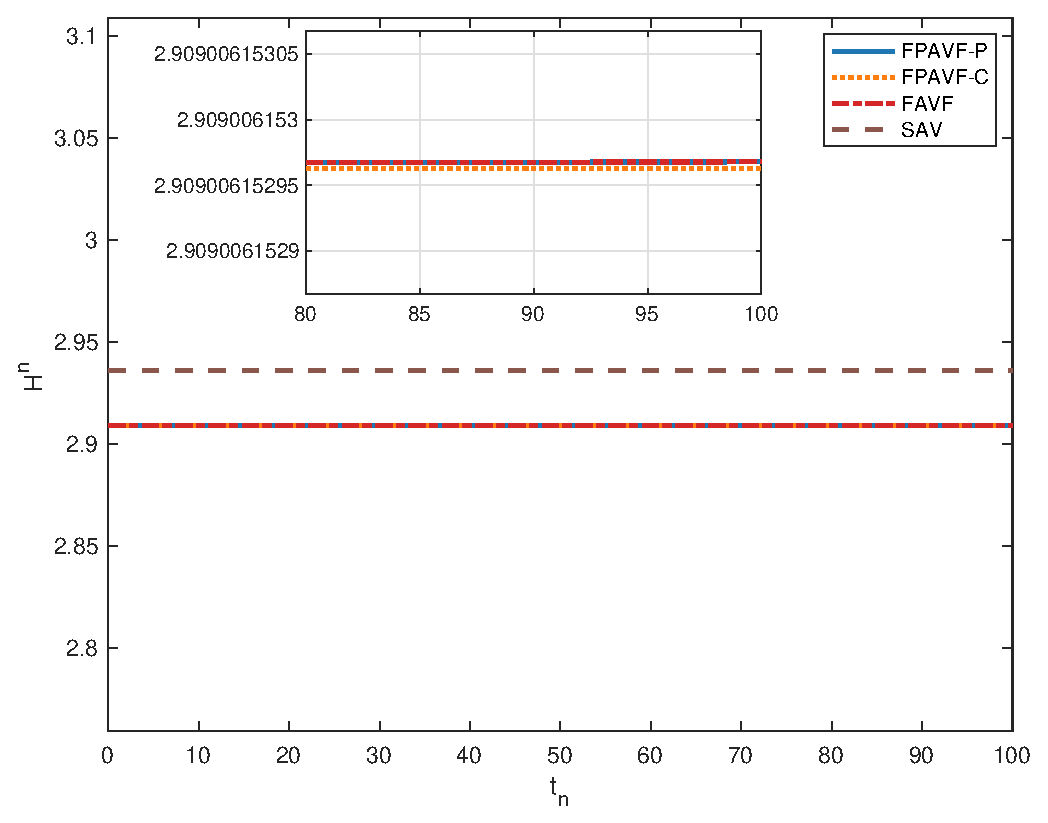
\includegraphics[width=0.3\textwidth]{./figure/exp2_H1.3.eps}
	%\centerline{($a$) $\alpha=1.3$}
	}\subfigure[$\alpha=1.6$]{ \centering
	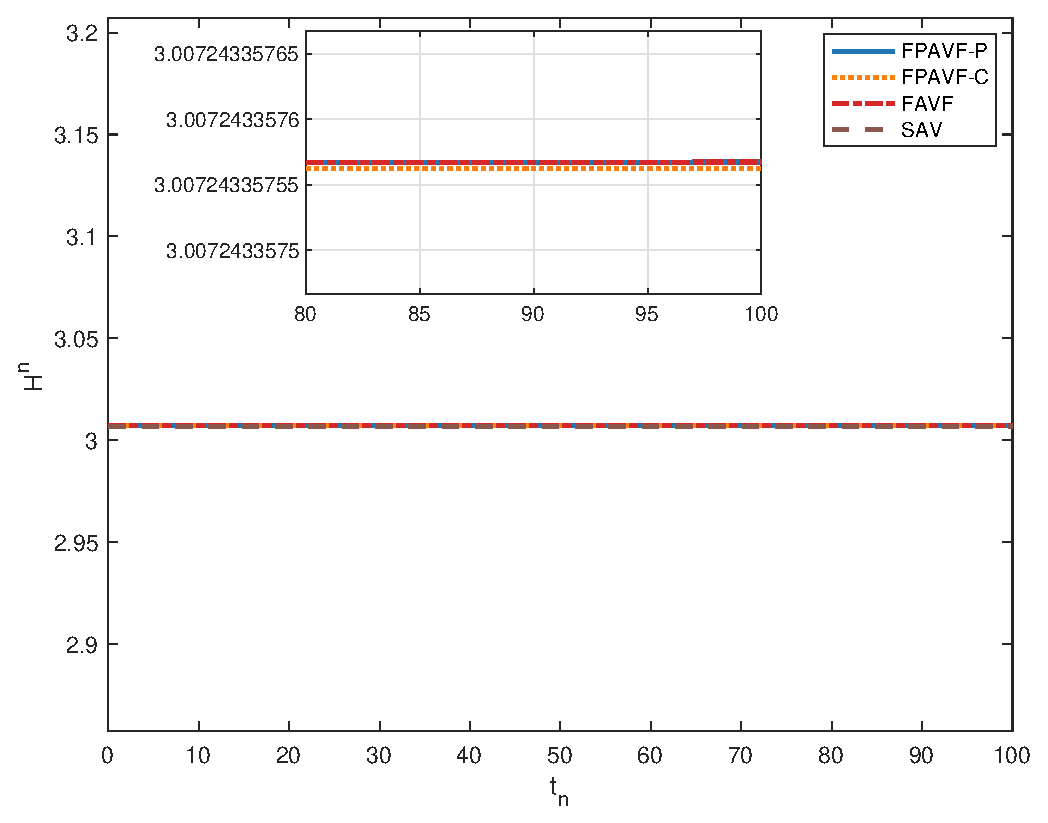
\includegraphics[width=0.3\textwidth]{./figure/exp2_H1.6.eps}
	%\centerline{($b$) $\alpha=1.6$}
	}\\
	\subfigure[$\alpha=1.9$]{ \centering
	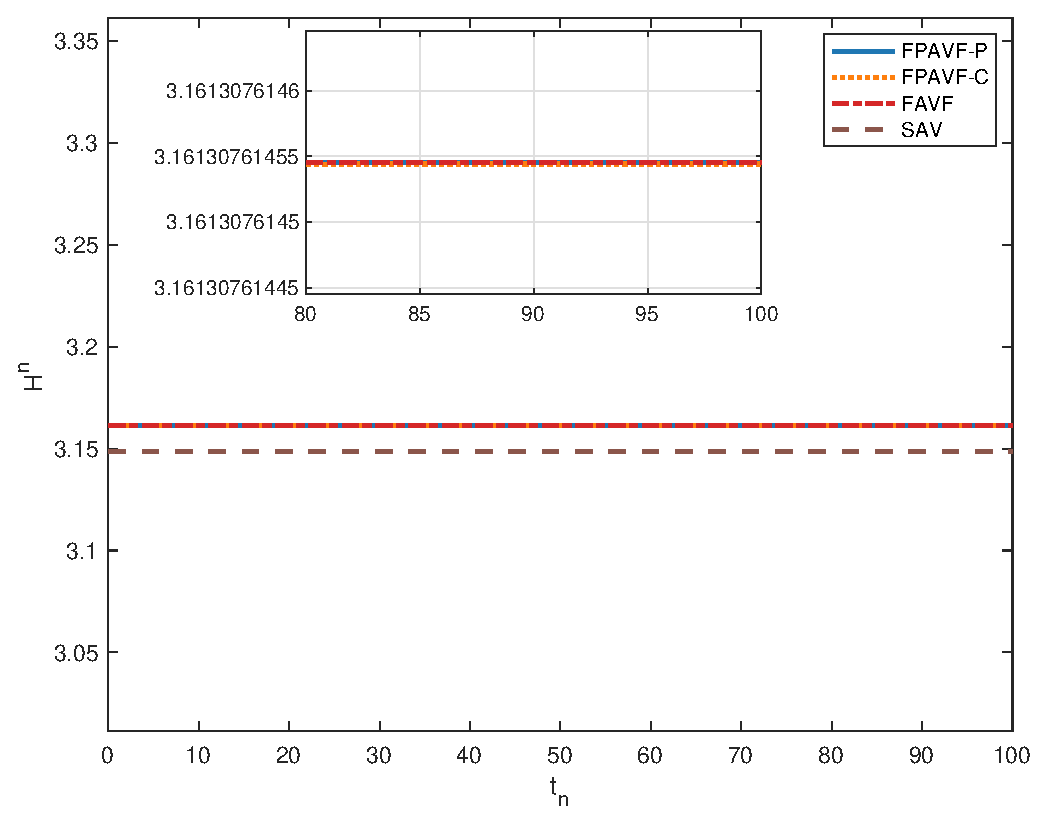
\includegraphics[width=0.3\textwidth]{./figure/exp2_H1.9.eps}
	%\centerline{($d$) $\alpha=2.0$}
	}\subfigure[$\alpha=2.0$]{ \centering
	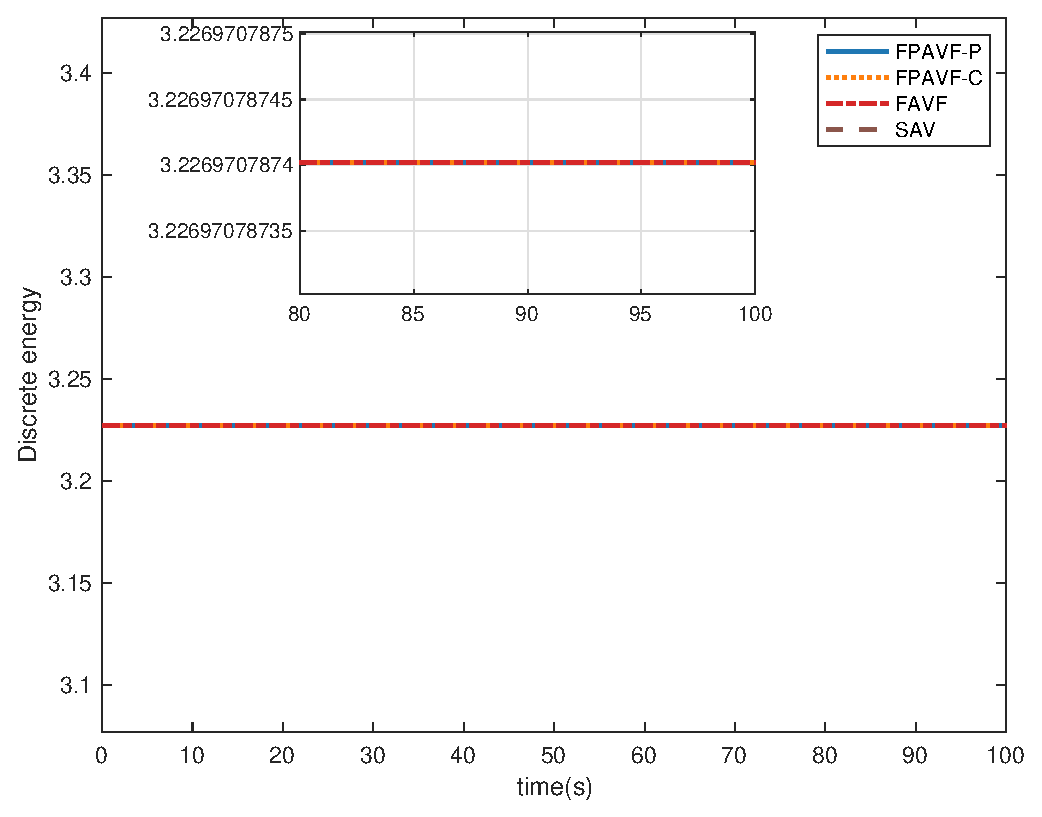
\includegraphics[width=0.3\textwidth]{./figure/exp2_H2.eps}
	%\centerline{($d$) $\alpha=2.0$}
	}
	% \caption{Discrete energy for different $\alpha$ in Example \ref{exp_PAVF:4} with $N = 64$ and $\tau=0.01$.} 
	\caption{在例 \ref{exp_PAVF:4} 中,当 $N = 64$ 且 $\tau=0.01$ 时,不同 $\alpha$ 下的离散能量.}
	\label{fig_PAVF:10}
	\end{center}
	\end{figure}


\begin{figure}[H]
\begin{center}
 \subfigure[$\alpha=1.3$]{ \centering
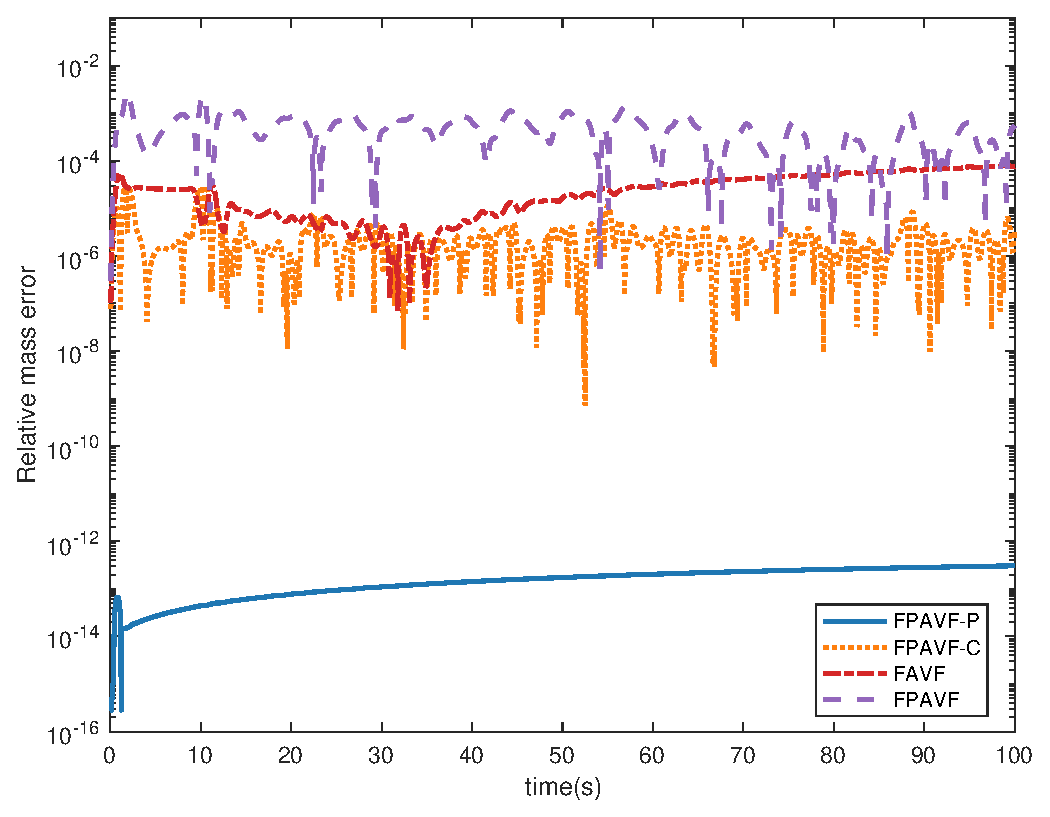
\includegraphics[width=0.3\textwidth]{./figure/exp2_RM1.3.eps}
%\centerline{($a$) $\alpha=1.3$}
}\subfigure[$\alpha=1.6$]{ \centering
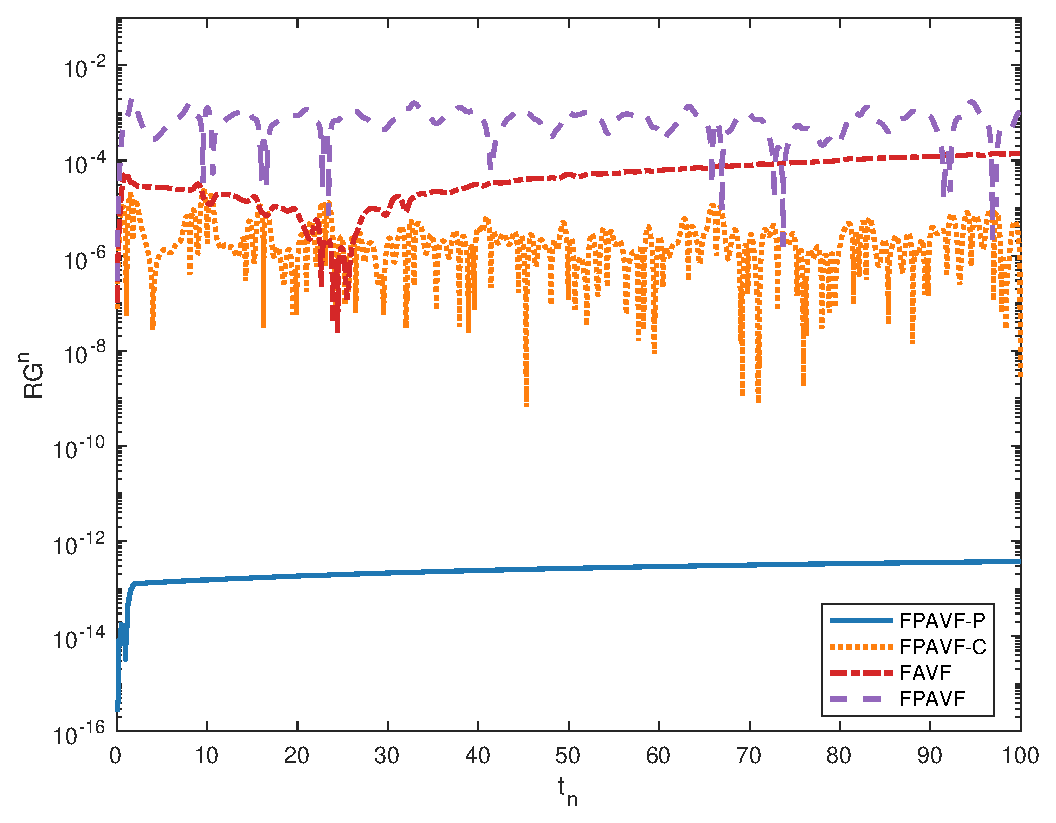
\includegraphics[width=0.3\textwidth]{./figure/exp2_RM1.6.eps}
%\centerline{($b$) $\alpha=1.6$}
}\subfigure[$\alpha=1.9$]{ \centering
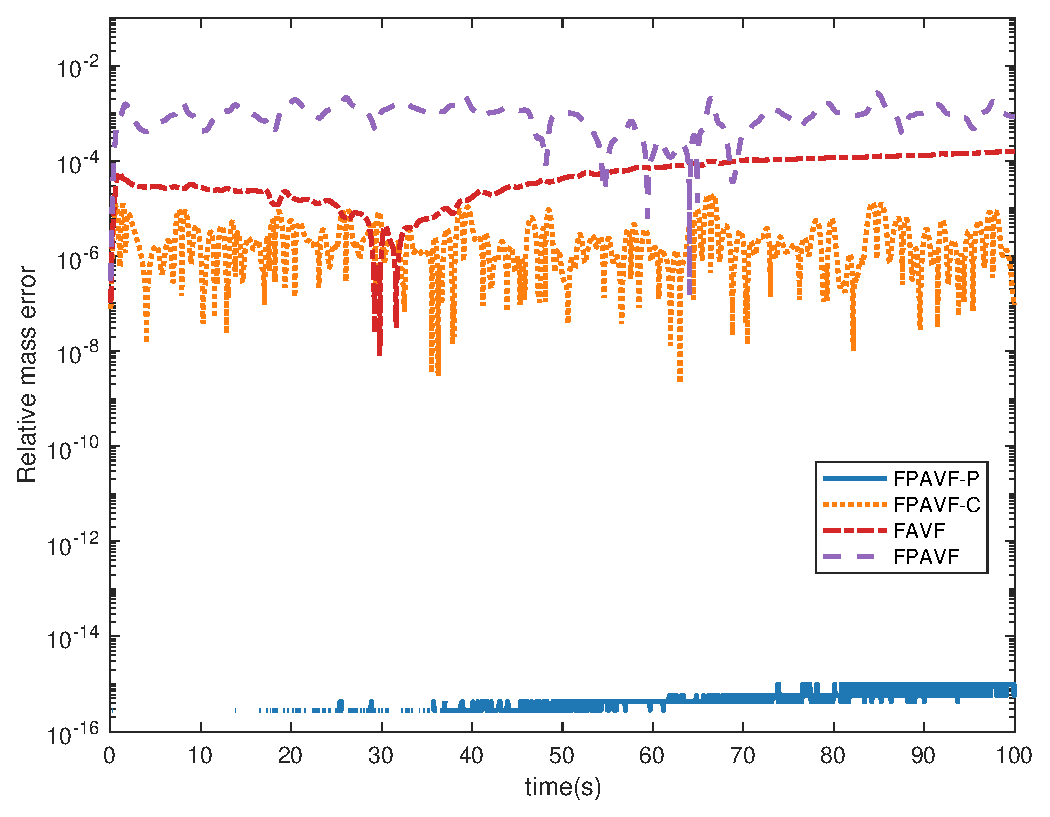
\includegraphics[width=0.3\textwidth]{./figure/exp2_RM1.9.eps}
%\centerline{($c$) $\alpha=1.9$}
}
% \caption{The relative errors of discrete mass for different $\alpha$ in Example \ref{exp_PAVF:4} with $N = 64$ and $\tau=0.01$.} 
\caption{在例 \ref{exp_PAVF:4} 中,当 $N = 64$ 且 $\tau=0.01$ 时,不同 $\alpha$ 下的离散质量相对误差}
\label{fig_PAVF:11}
\end{center}
\end{figure}


\begin{figure}[H]
\begin{center}
 \subfigure[$\alpha=1.3$]{ \centering
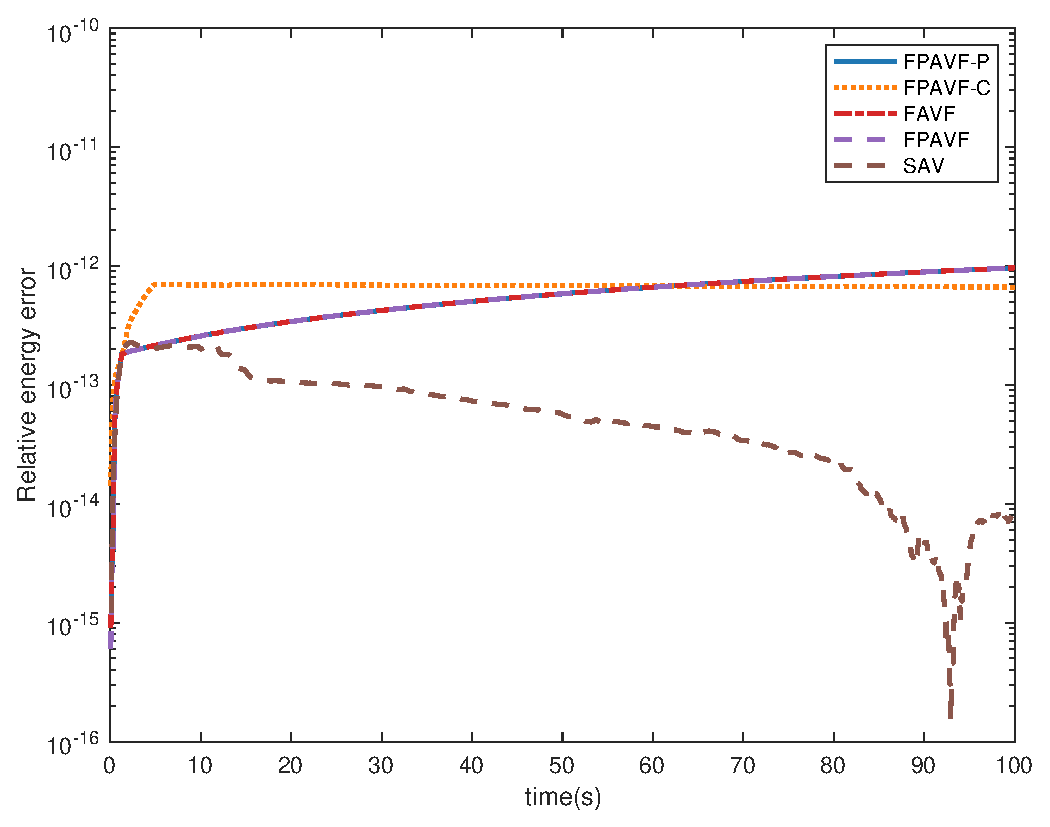
\includegraphics[width=0.3\textwidth]{./figure/exp2_RH1.3.eps}
%\centerline{($a$) $\alpha=1.3$}
}\subfigure[$\alpha=1.6$]{ \centering
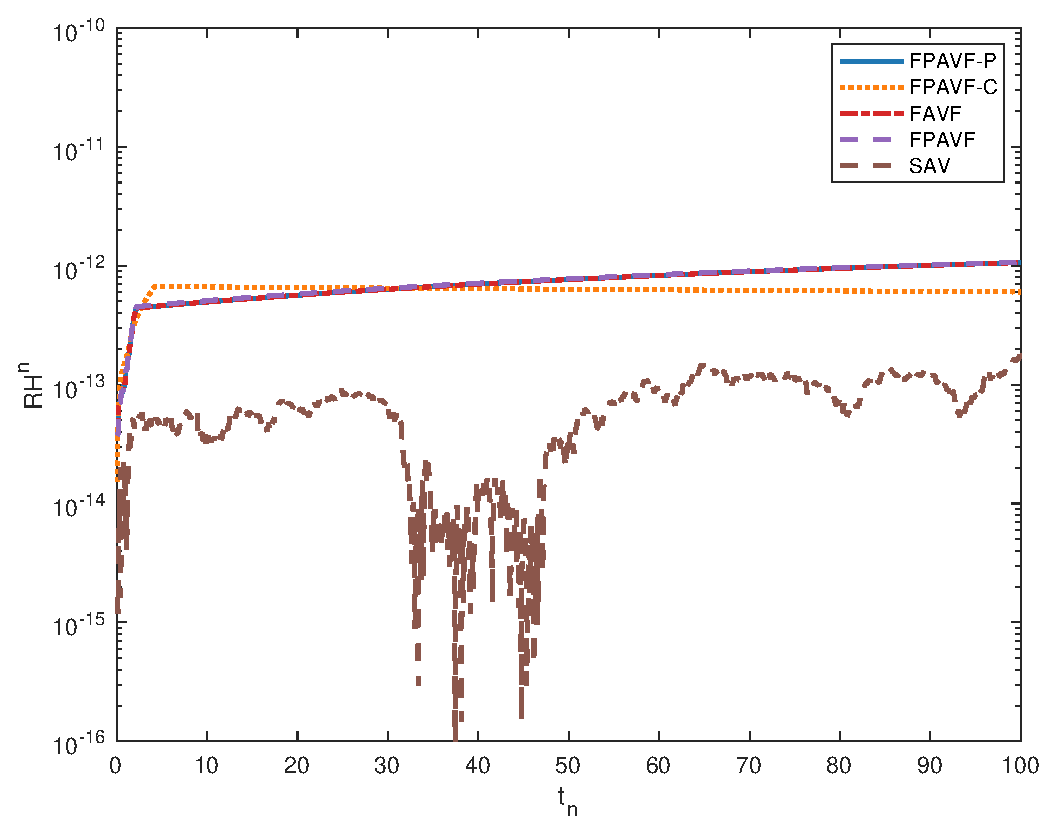
\includegraphics[width=0.3\textwidth]{./figure/exp2_RH1.6.eps}
%\centerline{($b$) $\alpha=1.6$}
} \subfigure[$\alpha=1.9$]{ \centering
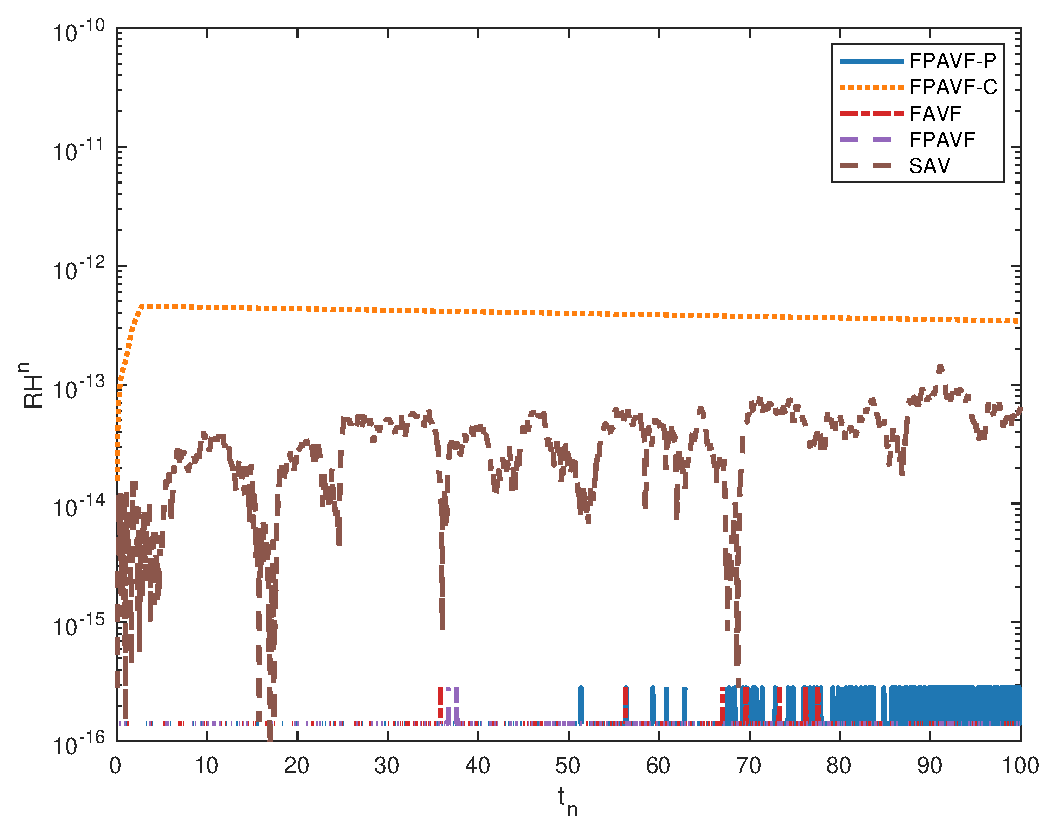
\includegraphics[width=0.3\textwidth]{./figure/exp2_RH1.9.eps}
%\centerline{($c$) $\alpha=1.9$}
}
% \caption{The relative errors of discrete energy for different $\alpha$ in Example \ref{exp_PAVF:4} with $N = 64$ and $\tau=0.01$.} 
\caption{在例 \ref{exp_PAVF:4} 中,当 $N = 64$ 且 $\tau=0.01$ 时,不同 $\alpha$ 下的离散能量相对误差}
\label{fig_PAVF:12}
\end{center}
\end{figure}

更详细的比较结果见表 \ref{tab_PAVF:4-1} 到表 \ref{tab_PAVF:4-4},通过观察这些数据,我们可以得出相同的结论.


\begin{table}[H]\small
	\centering
	% \caption{Discrete energy $H^n$ at time $t=t_n$ for Example \ref{exp_PAVF:4} when $\alpha=2$.}
	\caption{在例 \ref{exp_PAVF:4} 中,当 $\alpha=2.0$ 时,时刻 $t=t_n$ 的离散能量 $H^n$.}
	\begin{tabular}{llllll}
	  \toprule
       $t$   &FAVF   &FPAVF   &FPAVF-C   &SAV   &FPAVF-P\\
	  \midrule
	  0     & 3.22697078740176 & 3.22697078740176 & 3.22697078740173 & 3.21234862767094 & 3.22697078740176 \\
	  10    & 3.22697078740176 & 3.22697078740176 & 3.22697078740168 & 3.21234862767062 & 3.22697078740176 \\
	  20    & 3.22697078740176 & 3.22697078740176 & 3.22697078740172 & 3.21234862767066 & 3.22697078740176 \\
	  40    & 3.22697078740175 & 3.22697078740176 & 3.22697078740182 & 3.21234862767033 & 3.22697078740176 \\
	  60    & 3.22697078740176 & 3.22697078740176 & 3.22697078740191 & 3.21234862767035 & 3.22697078740176 \\
	  80    & 3.22697078740176 & 3.22697078740175 & 3.22697078740199 & 3.21234862767073 & 3.22697078740176 \\
	  100   & 3.22697078740175 & 3.22697078740176 & 3.22697078740207 & 3.21234862767045 & 3.22697078740176 \\
	  \midrule
	  \multicolumn{6}{r}{Original energy:~3.22697078976648} \\
	  \bottomrule
	  \end{tabular}\label{tab_PAVF:4-1}%
  \end{table}%


  % Table generated by Excel2LaTeX from sheet 'Sheet1'
\begin{table}[H]\small
	\centering
	% \caption{Discrete mass $G^n$ at time $t=t_n$ for Example \ref{exp_PAVF:4} when $\alpha=1.3$.}
	\caption{在例 \ref{exp_PAVF:4} 中,当 $\alpha=1.3$ 时,时刻 $t=t_n$ 的离散质量 $G^n$.}
	  \begin{tabular}{lllll}
	  \toprule
$t$   &FAVF   &FPAVF   &FPAVF-C   &FPAVF-P\\
	  \midrule
	  0     & 3.14159297667455 & 3.14159361842152 & 3.14159241227909 & 3.14159265358976 \\
	  10    & 3.14160952253933 & 3.13595374862870 & 3.14166505643569 & 3.14159265358963 \\
	  20    & 3.14161343543099 & 3.14421089321261 & 3.14158965037808 & 3.14159265358952 \\
	  40    & 3.14157539023564 & 3.14362067013654 & 3.14159917106759 & 3.14159265358932 \\
	  60    & 3.14150249358846 & 3.14217508702013 & 3.14159868539556 & 3.14159265358912 \\
	  80    & 3.14143174175214 & 3.14159826267015 & 3.14158946625201 & 3.14159265358895 \\
	  100   & 3.14135672071641 & 3.14328710863969 & 3.14158227319751 & 3.14159265358880 \\
	  \midrule
	  \multicolumn{5}{r}{Original mass:~3.14159265323701} \\
	  \bottomrule
	  \end{tabular}\label{tab_PAVF:4-2}%
  \end{table}%

  % Table generated by Excel2LaTeX from sheet 'Sheet1'
\begin{table}[H]\small
	\centering
	% \caption{Discrete mass $G^n$ at time $t=t_n$ for Example \ref{exp_PAVF:4} when $\alpha=1.6$.}
	\caption{在例 \ref{exp_PAVF:4} 中,当 $\alpha=1.6$ 时,时刻 $t=t_n$ 的离散质量 $G^n$.}
	 \begin{tabular}{lllll}
	  \toprule
$t$   &FAVF   &FPAVF   &FPAVF-C   &FPAVF-P\\
	  \midrule
	  0     & 3.14159297668940 & 3.14159361814729 & 3.14159241218683 & 3.14159265358976 \\
	  10    & 3.14163389358031 & 3.13754191888209 & 3.14160072631792 & 3.14159265358928 \\
	  20    & 3.14161716177523 & 3.14433222488425 & 3.14159044899067 & 3.14159265358919 \\
	  40    & 3.14149554093894 & 3.14475213344308 & 3.14160500647197 & 3.14159265358901 \\
	  60    & 3.14139997924855 & 3.14288256207779 & 3.14160023436812 & 3.14159265358885 \\
	  80    & 3.14127488637752 & 3.14241392600216 & 3.14158768432513 & 3.14159265358871 \\
	  100   & 3.14115287766347 & 3.14489331385338 & 3.14159412822417 & 3.14159265358860 \\
		\midrule
	  \multicolumn{5}{r}{Original mass:~3.14159265323701} \\
	  \bottomrule
	  \end{tabular}\label{tab_PAVF:4-3}%
  \end{table}%

  % Table generated by Excel2LaTeX from sheet 'Sheet1'
\begin{table}[H]\small
	\centering
	% \caption{Discrete mass $G^n$ at time $t=t_n$ for Example \ref{exp_PAVF:4} when $\alpha=2$.}
	\caption{在例 \ref{exp_PAVF:4} 中,当 $\alpha=2.0$ 时,时刻 $t=t_n$ 的离散质量 $G^n$.}
	\begin{tabular}{lllll}
	  \toprule
$t$   &FAVF   &FPAVF   &FPAVF-C   &FPAVF-P\\
	  \midrule
	  0     & 3.14159297725470 & 3.14159361919902 & 3.14159241149324 & 3.14159265358976 \\
	  10    & 3.14168000260412 & 3.14369215006721 & 3.14160070161208 & 3.14159265358976 \\
	  20    & 3.14164544531849 & 3.14521250122401 & 3.14158745249453 & 3.14159265358976 \\
	  40    & 3.14150535695500 & 3.14531702832209 & 3.14160031804829 & 3.14159265358976 \\
	  60    & 3.14136438511727 & 3.14552013864766 & 3.14159560564481 & 3.14159265358976 \\
	  80    & 3.14118013227991 & 3.14739329967543 & 3.14158800109644 & 3.14159265358976 \\
	  100   & 3.14101125059928 & 3.15011874273391 & 3.14154787019595 & 3.14159265358976 \\
	  \midrule
	  \multicolumn{5}{r}{Original mass:~3.14159265323701} \\
	  \bottomrule
	  \end{tabular}\label{tab_PAVF:4-4}%
  \end{table}%

  最后,我们分别在图 \ref{fig_PAVF:13}-\ref{fig_PAVF:16} 中展示了 $\alpha=1.3,1.6,1.99,2$ 时波的演化过程,这是通过取 $N=128$ 和 $\tau=0.01$ 得到的.我们可以观察到,阶数 $\alpha$ 将显著影响波的形状,当 $\alpha$ 变大时,波的形状变化更快.具体来说,当 $\alpha \rightarrow 2$ 时,数值解收敛到经典的非线性薛定谔波动方程,参见 \cite{zhangConservativeNumericalScheme2003,liCompactFiniteDifference2012,wangAnalysisNewConservative2006}.

  \begin{figure}[H]
	\begin{center}
	 \subfigure[$t=0s$]{ \centering
	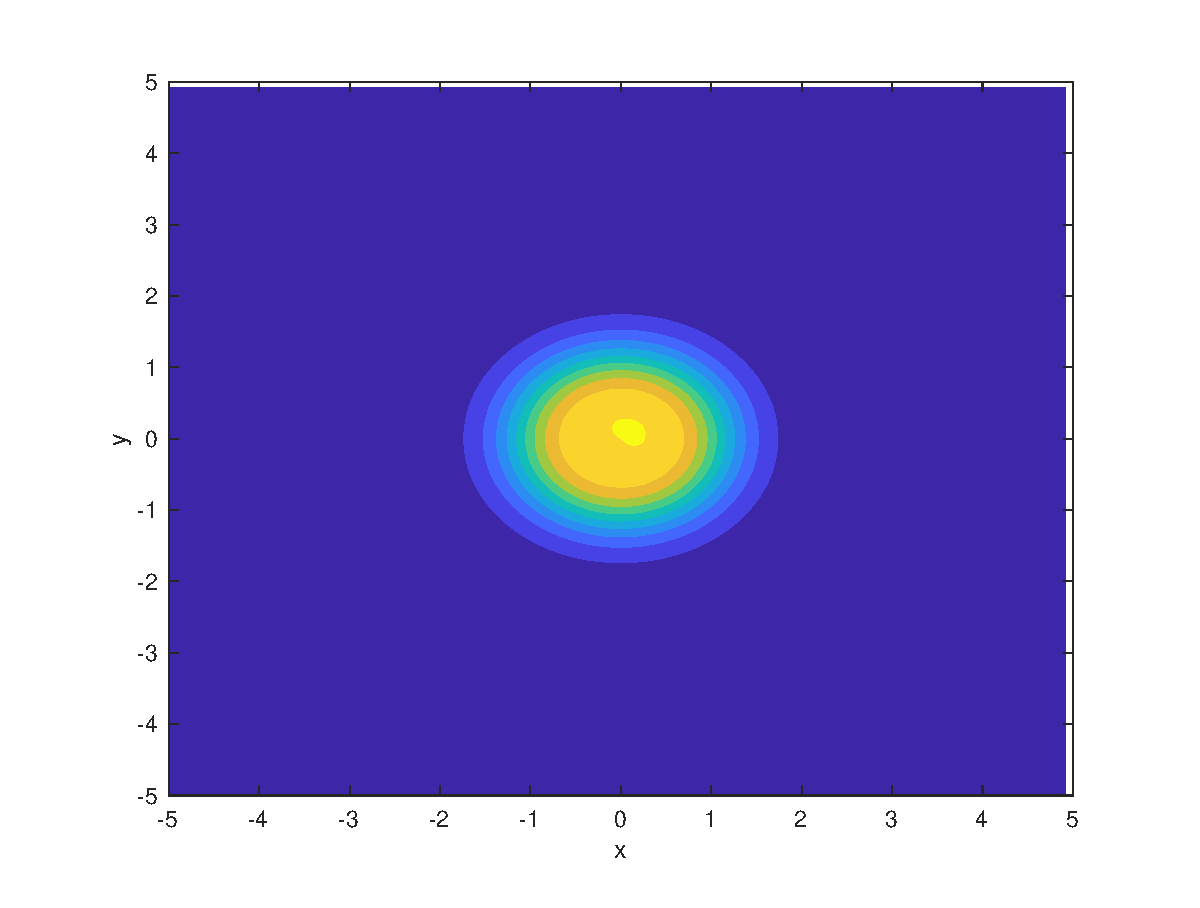
\includegraphics[width=0.3\textwidth]{./figure/exp2_contour3_p0.eps}
	}\subfigure[$t=1s$]{ \centering
	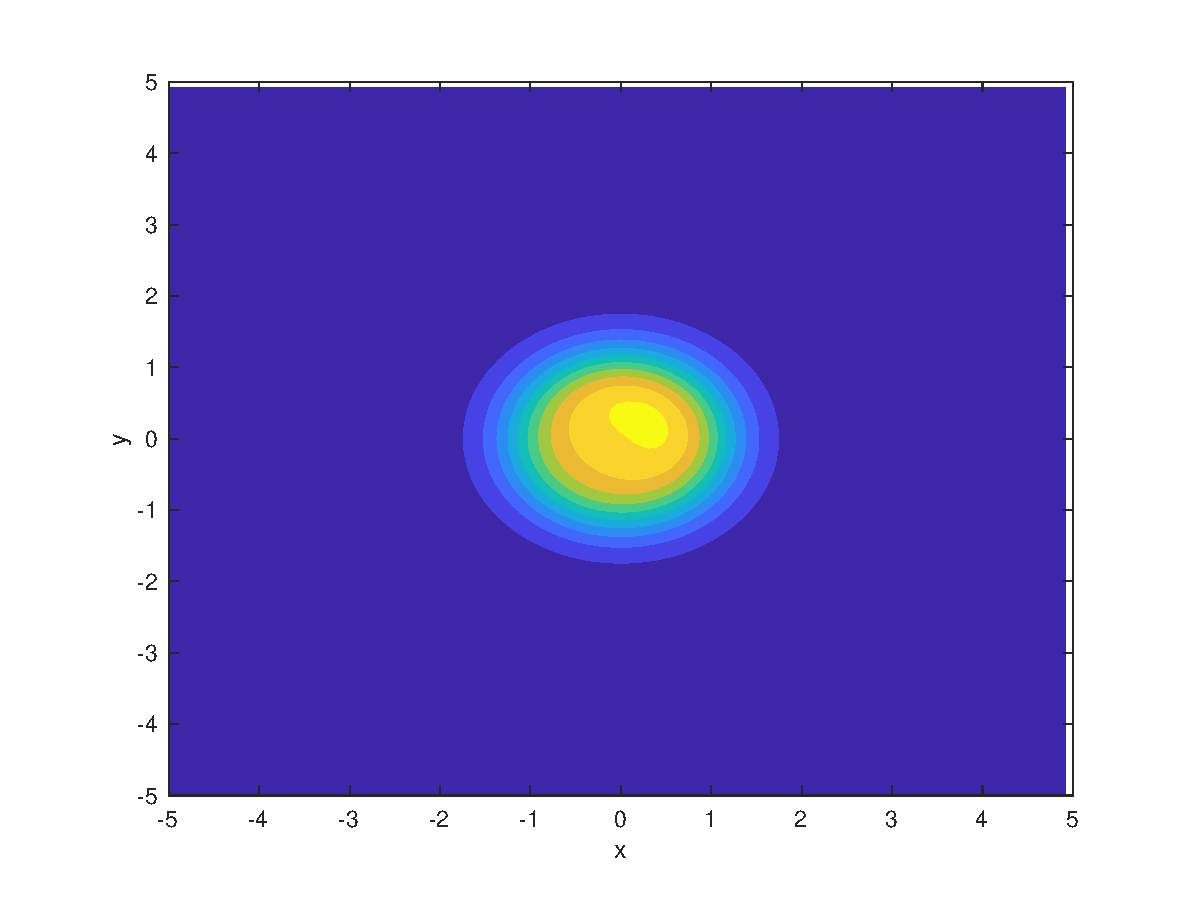
\includegraphics[width=0.3\textwidth]{./figure/exp2_contour3_p1.eps}
	} \subfigure[$t=5s$]{ \centering
	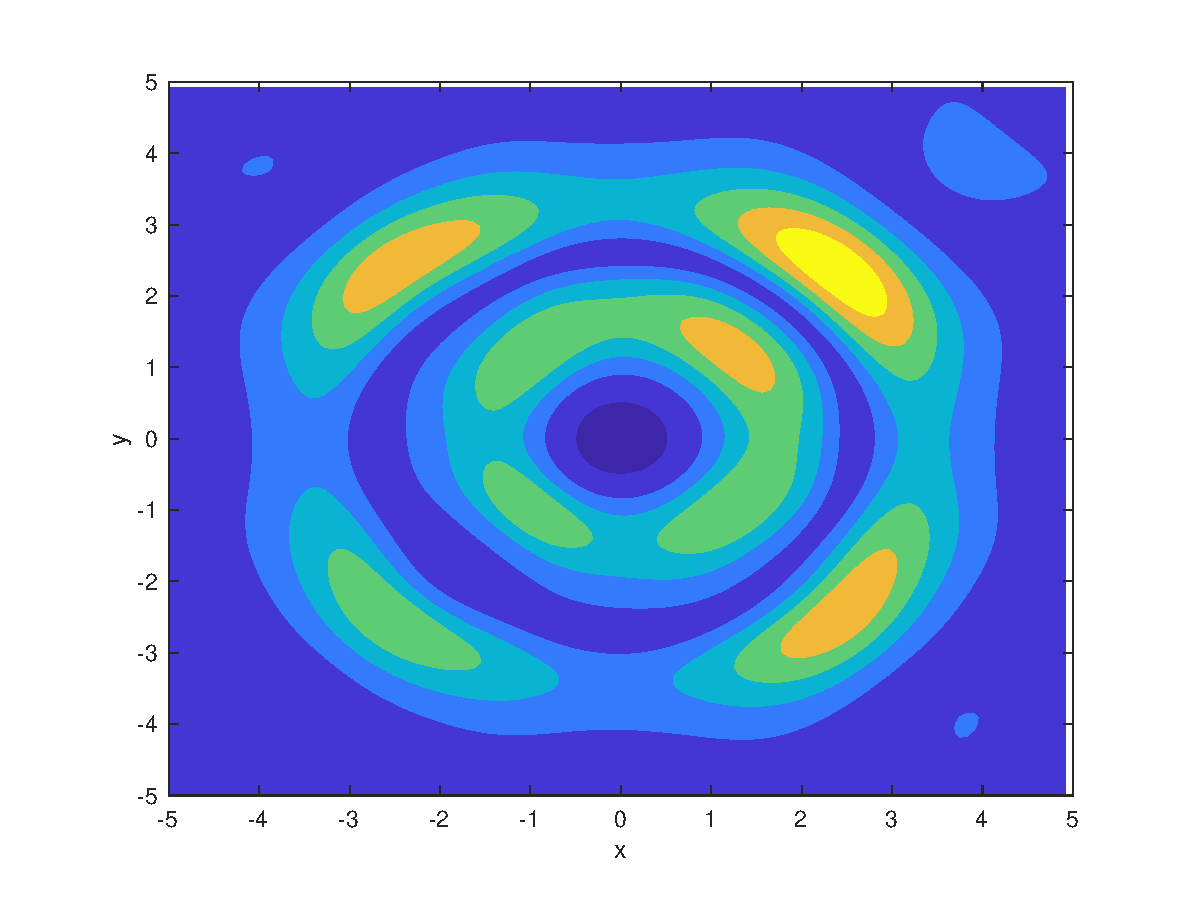
\includegraphics[width=0.3\textwidth]{./figure/exp2_contour3_p5.eps}
	}\\
	\subfigure[$t=10s$]{ \centering
	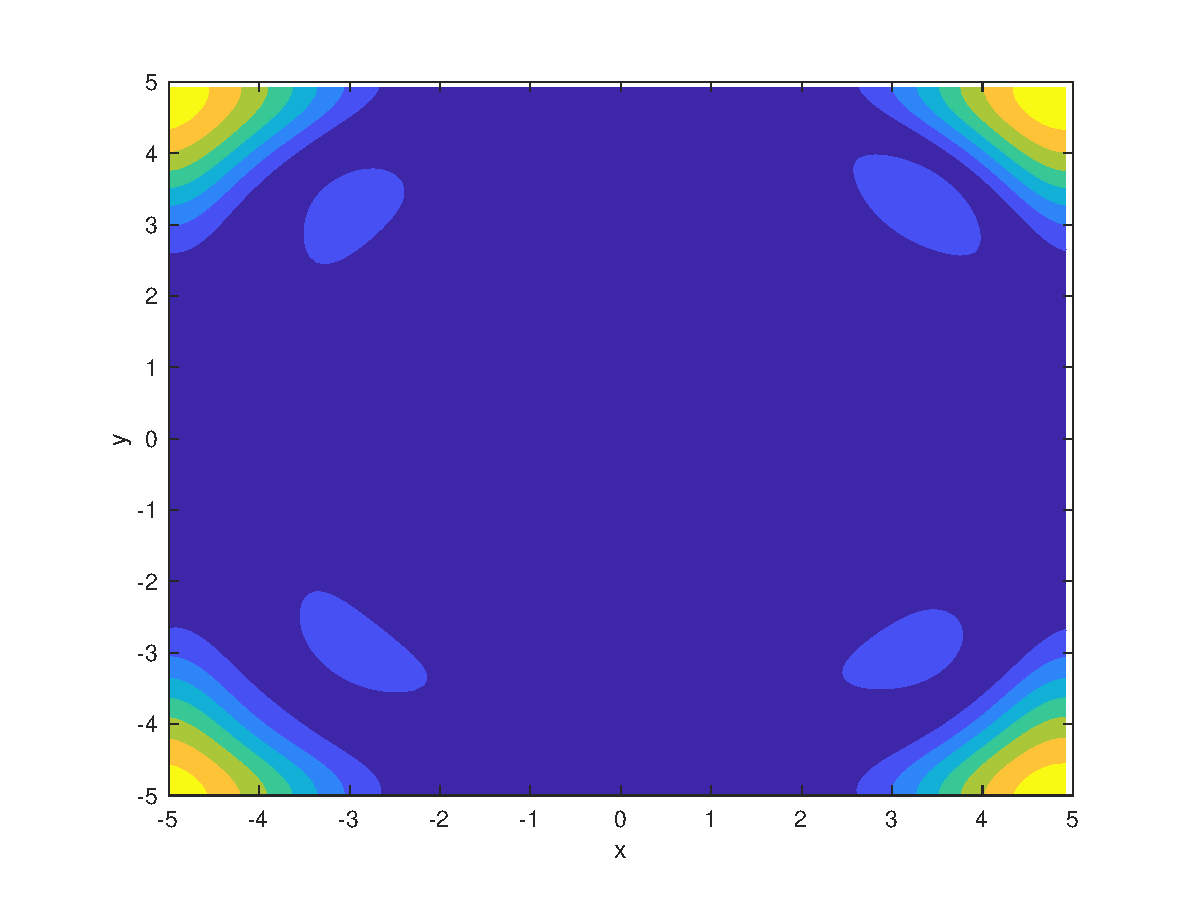
\includegraphics[width=0.3\textwidth]{./figure/exp2_contour3_p10.eps}
	}\subfigure[$t=50s$]{ \centering
	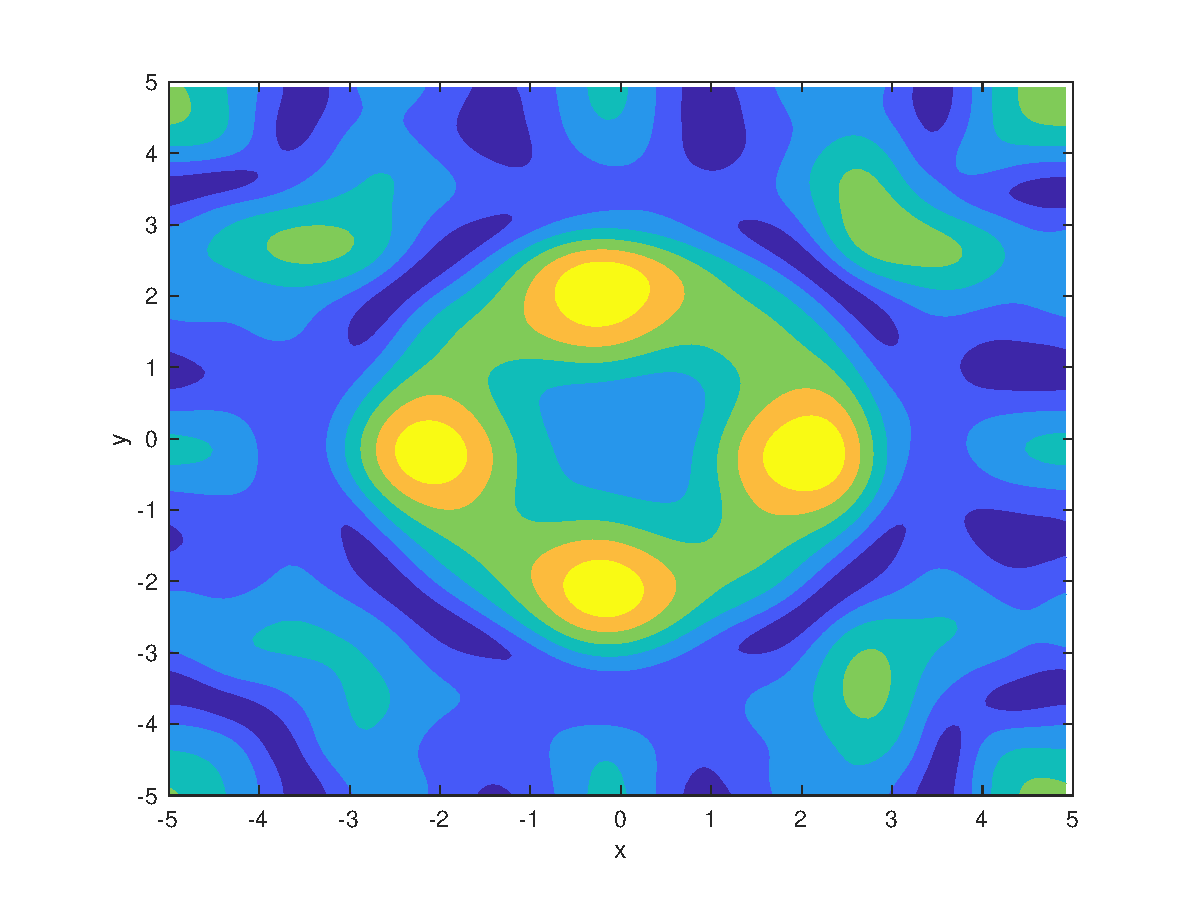
\includegraphics[width=0.3\textwidth]{./figure/exp2_contour3_p50.eps}
	} \subfigure[$t=100s$]{ \centering
	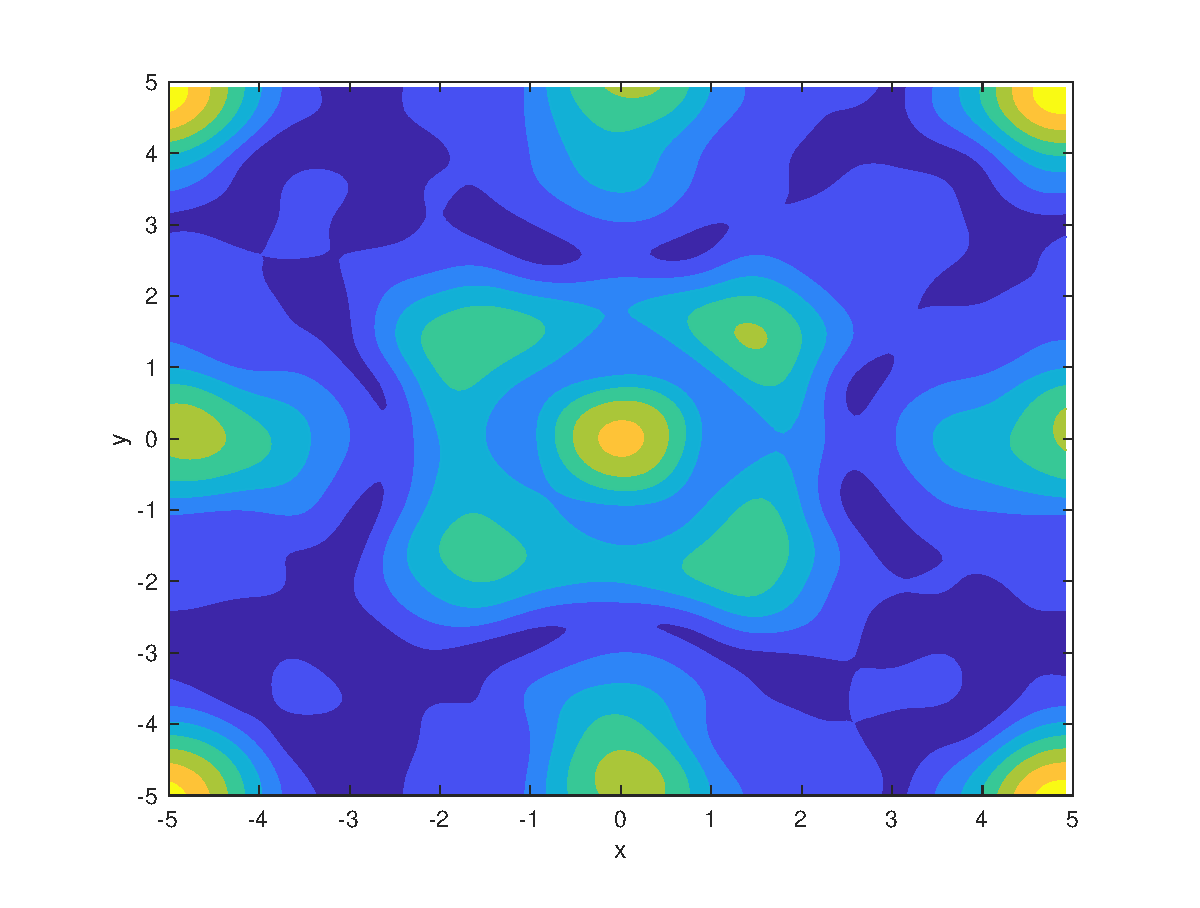
\includegraphics[width=0.3\textwidth]{./figure/exp2_contour3_p100.eps}
	}
	\caption{示例 \ref{exp_PAVF:4} 中,$\alpha=1.3$ 时的波传播图.}
	% \caption{The pictures of wave propagation for Example \ref{exp_PAVF:4} with $\alpha=1.3.$}
	\label{fig_PAVF:13}
	\end{center}
	\end{figure}

	\begin{figure}[H]
		\begin{center}
		 \subfigure[$t=0s$]{ \centering
		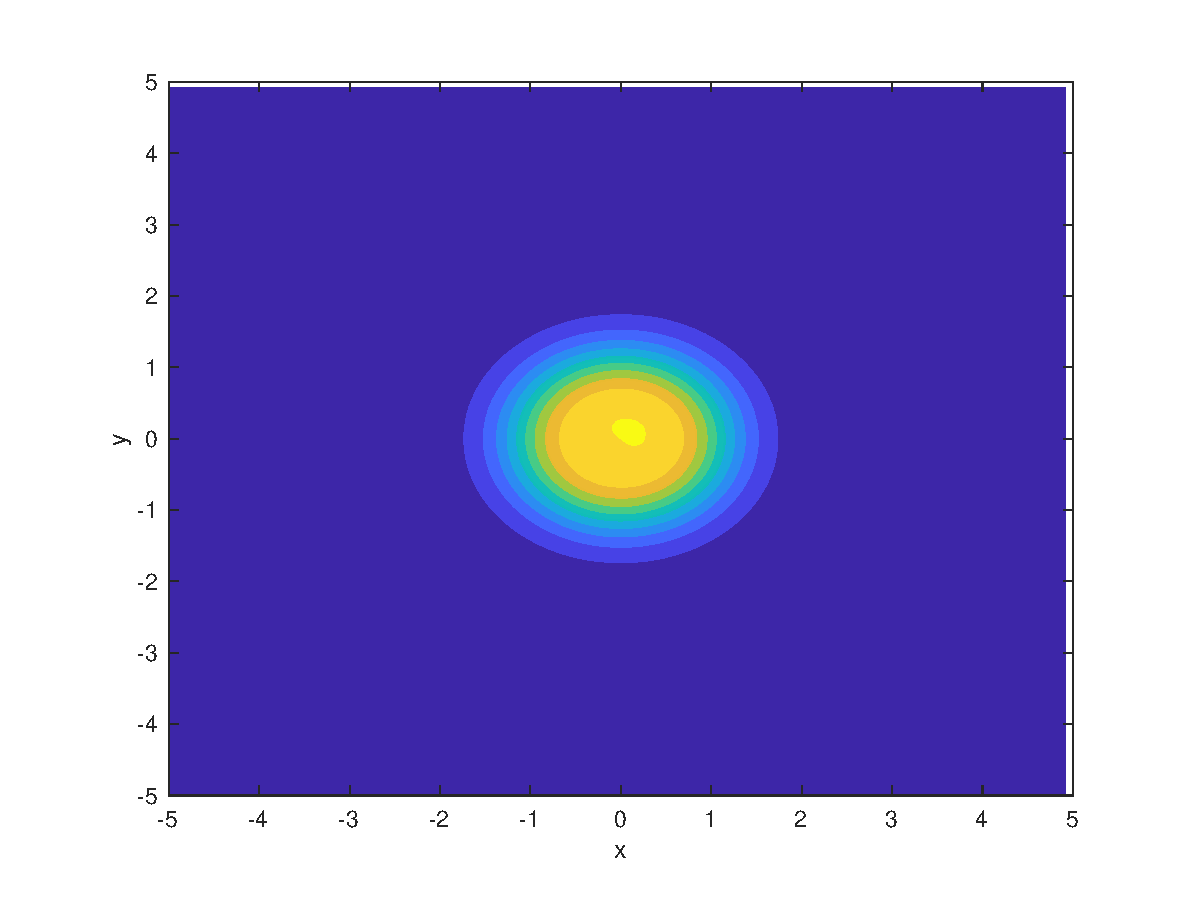
\includegraphics[width=0.3\textwidth]{./figure/exp2_contour6_p0.eps}
		}\subfigure[$t=1s$]{ \centering
		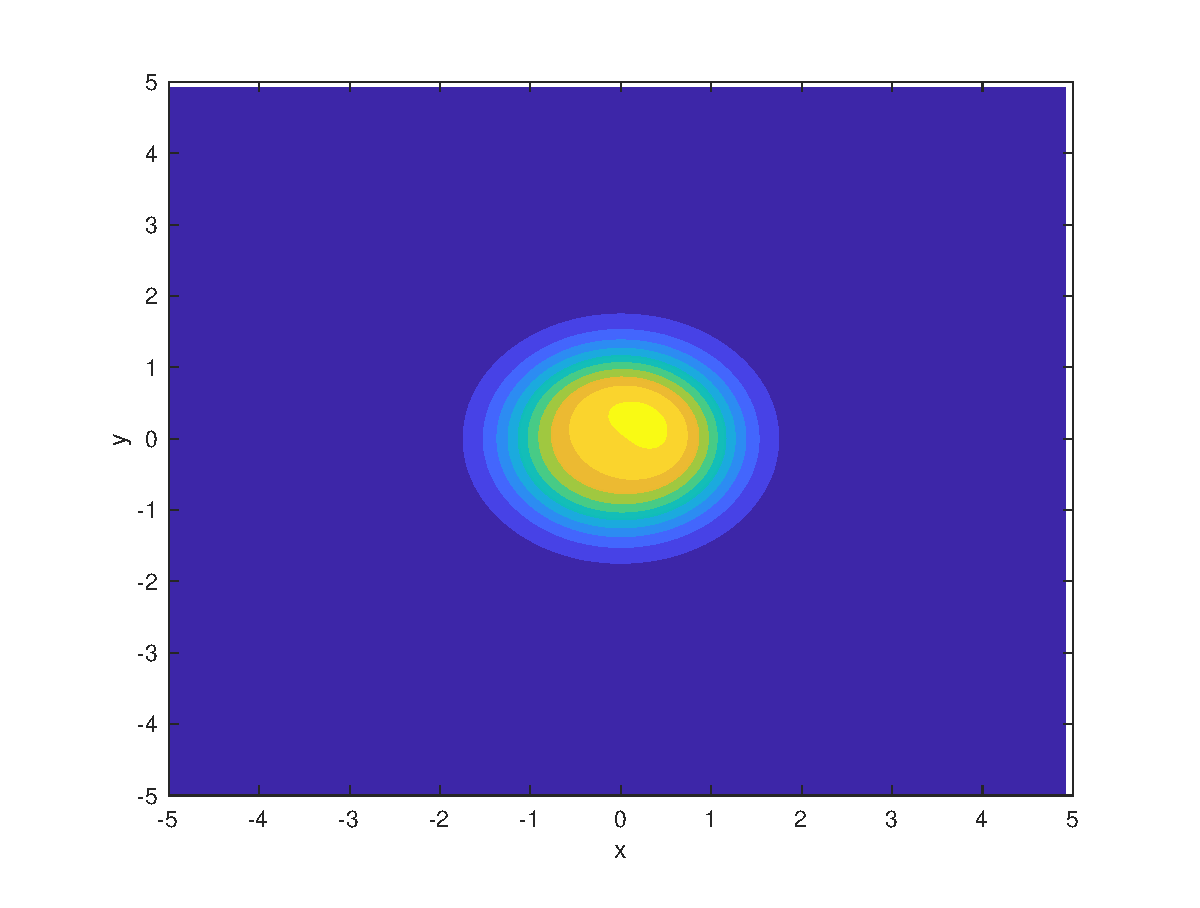
\includegraphics[width=0.3\textwidth]{./figure/exp2_contour6_p1.eps}
		} \subfigure[$t=5s$]{ \centering
		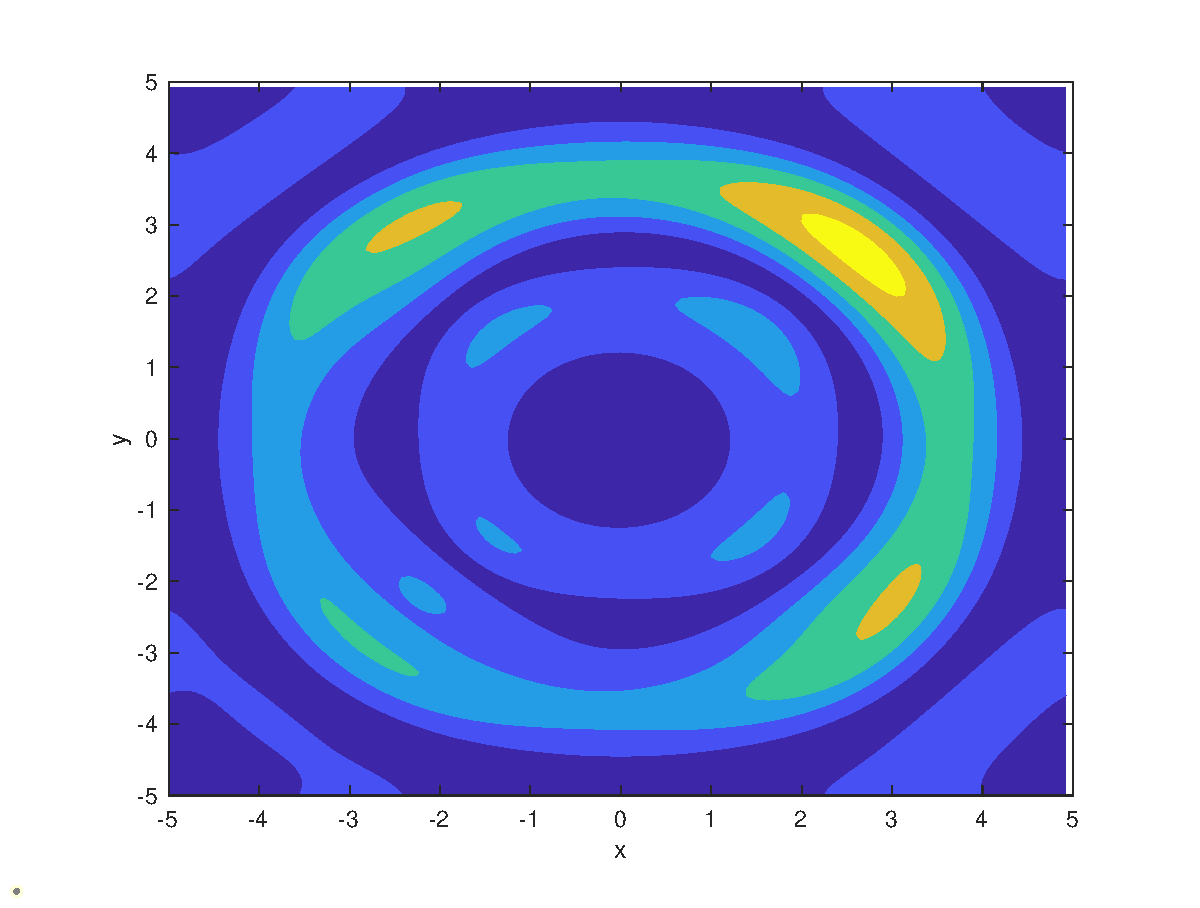
\includegraphics[width=0.3\textwidth]{./figure/exp2_contour6_p5.eps}
		}\\
		\subfigure[$t=10s$]{ \centering
		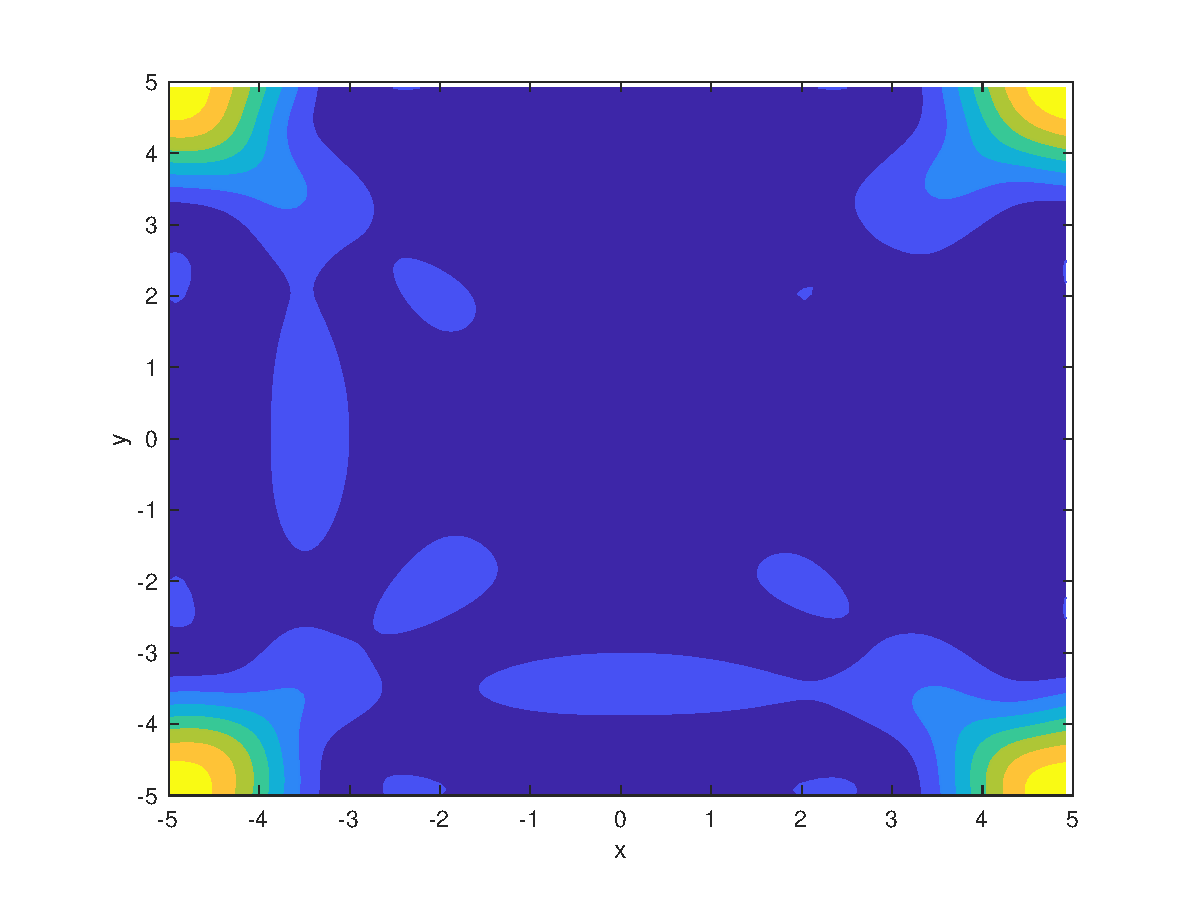
\includegraphics[width=0.3\textwidth]{./figure/exp2_contour6_p10.eps}
		}\subfigure[$t=50s$]{ \centering
		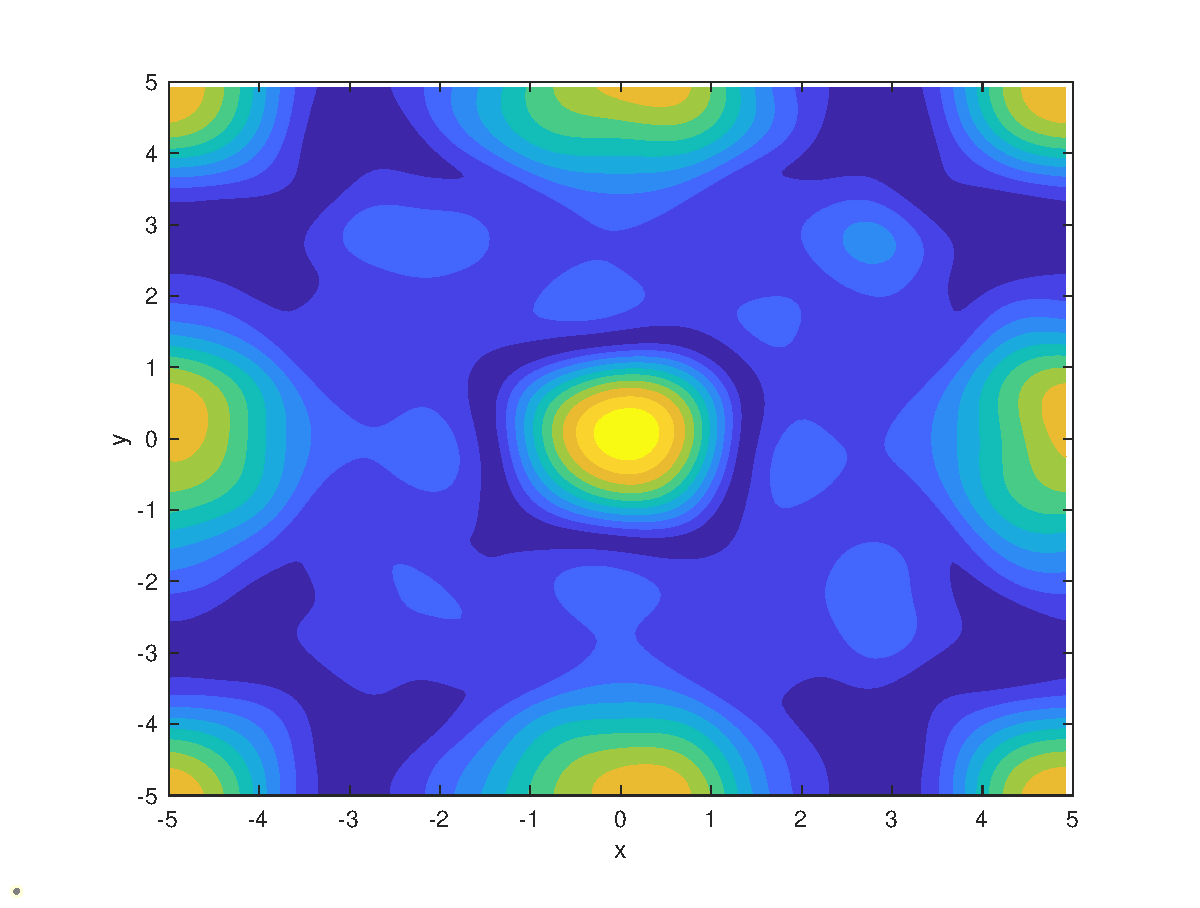
\includegraphics[width=0.3\textwidth]{./figure/exp2_contour6_p50.eps}
		} \subfigure[$t=100s$]{ \centering
		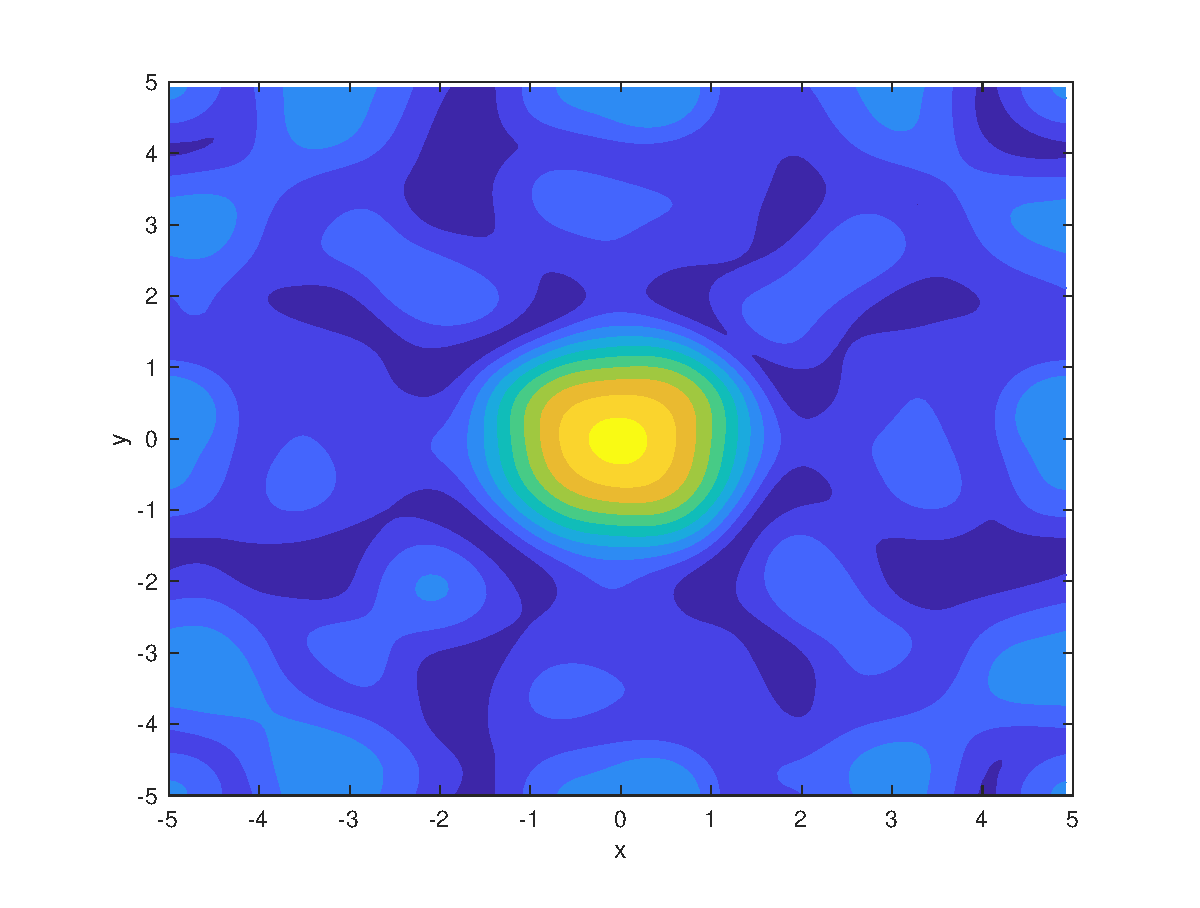
\includegraphics[width=0.3\textwidth]{./figure/exp2_contour6_p100.eps}
		}
		% \caption{The pictures of wave propagation for Example \ref{exp_PAVF:4} with $\alpha=1.6.$}
		\caption{示例 \ref{exp_PAVF:4} 中,$\alpha=1.6$ 时的波传播图.}
		\label{fig_PAVF:14}
		\end{center}
		\end{figure}

		\begin{figure}[H]
			\begin{center}
			 \subfigure[$t=0s$]{ \centering
			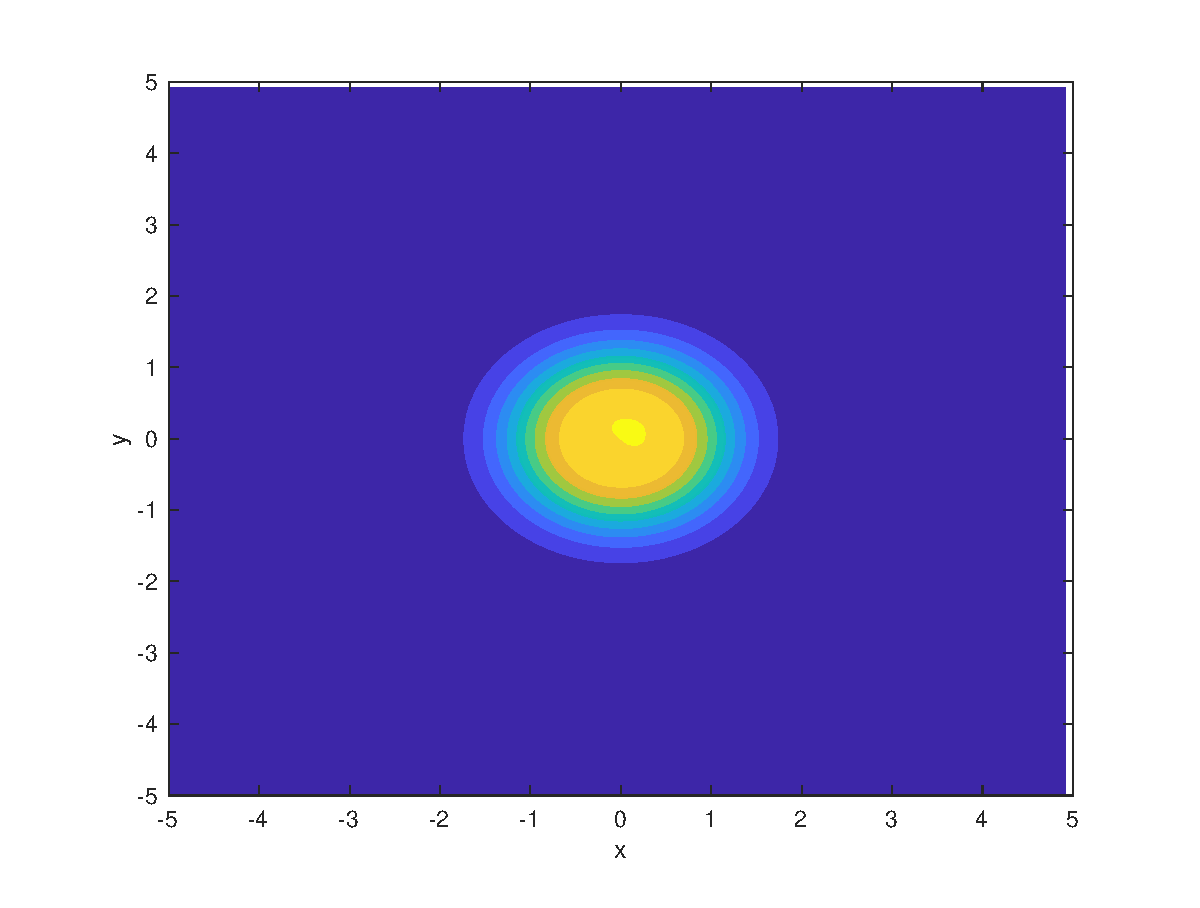
\includegraphics[width=0.3\textwidth]{./figure/exp2_contour99_p0.eps}
			}\subfigure[$t=1s$]{ \centering
			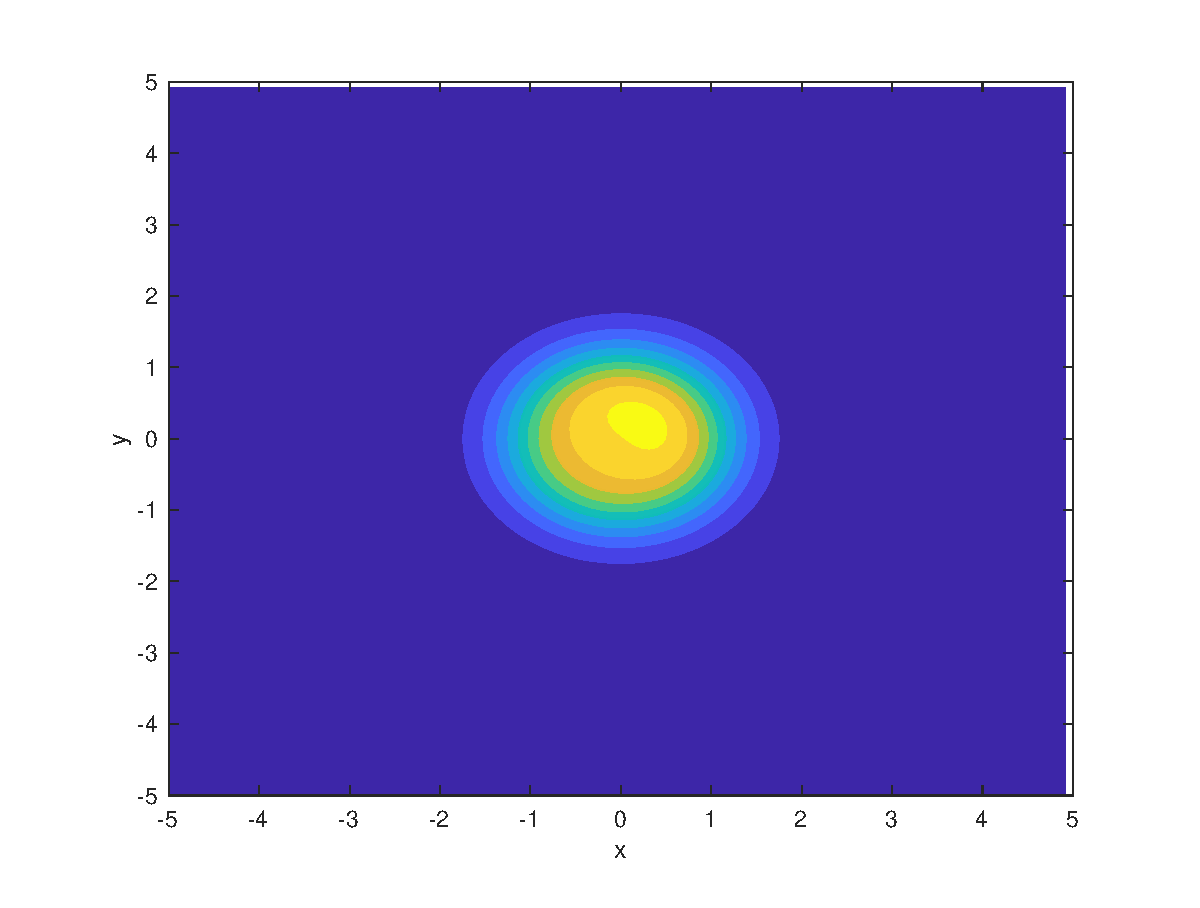
\includegraphics[width=0.3\textwidth]{./figure/exp2_contour99_p1.eps}
			} \subfigure[$t=5s$]{ \centering
			\includegraphics[width=0.3\textwidth]{./figure/exp2_contour99_p5.eps}
			}\\
			\subfigure[$t=10s$]{ \centering
			\includegraphics[width=0.3\textwidth]{./figure/exp2_contour99_p10.eps}
			}\subfigure[$t=50s$]{ \centering
			\includegraphics[width=0.3\textwidth]{./figure/exp2_contour99_p50.eps}
			} \subfigure[$t=100s$]{ \centering
			\includegraphics[width=0.3\textwidth]{./figure/exp2_contour99_p100.eps}
			}
			% \caption{The pictures of wave propagation for Example \ref{exp_PAVF:4} with $\alpha=1.99.$}
			\caption{示例 \ref{exp_PAVF:4} 中,$\alpha=1.99$ 时的波传播图.}
			\label{fig_PAVF:15}
			\end{center}
			\end{figure}
		
		%---------------------------------------------------------------------------------------------------------------------------
		\begin{figure}[H]
			\begin{center}
			 \subfigure[$t=0s$]{ \centering
			\includegraphics[width=0.3\textwidth]{./figure/exp2_contour2_p0.eps}
			}\subfigure[$t=1s$]{ \centering
			\includegraphics[width=0.3\textwidth]{./figure/exp2_contour2_p1.eps}
			} \subfigure[$t=5s$]{ \centering
			\includegraphics[width=0.3\textwidth]{./figure/exp2_contour2_p5.eps}
			}\\
			\subfigure[$t=10s$]{ \centering
			\includegraphics[width=0.3\textwidth]{./figure/exp2_contour2_p10.eps}
			}\subfigure[$t=50s$]{ \centering
			\includegraphics[width=0.3\textwidth]{./figure/exp2_contour2_p50.eps}
			} \subfigure[$t=100s$]{ \centering
			\includegraphics[width=0.3\textwidth]{./figure/exp2_contour2_p100.eps}
			}
			% \caption{The pictures of wave propagation for Example \ref{exp_PAVF:4} with $\alpha=2.$}
			\caption{示例 \ref{exp_PAVF:4} 中,$\alpha=2.0$ 时的波传播图.}
			\label{fig_PAVF:16}
			\end{center}
			\end{figure}

\section{小结}\label{Section_PAVF: 5}

在本文中,我们重新表述了二维分数非线性薛定谔波动方程为一个规范哈密顿系统.通过将分块平均向量场加方法与傅立叶拟谱方法结合,我们基于得到的哈密顿系统构建了一个保守的数值格式.理论分析和数值结果表明,所提出的方法能够有效地保持原始能量和质量.

% \section*{致谢}

% 本工作得到了四川省科技计划(No. 2022JDTD0019)的支持,以及四川师范大学劳伦数学中心和系统可信性自动验证国家地方联合工程实验室(资助号:ZD20220105)的支持.
	